% $Author: black $
% $Date: 2009-10-15 03:37:33 +0600 (чт, 15 окт 2009) $
% $Revision: 29460 $

% HISTORY:
% 2006-12-07 - Stef starts
% 2007-01-26 - Andrew updates
% 2007-05-22 - Andrew first draft
% 2007-06-24 - Oscar edit
% 2009-07-06 - Oscar migrate to pharo

%=================================================================
\ifx\wholebook\relax\else
% --------------------------------------------
% Lulu:
	\documentclass[a4paper,10pt,twoside]{book}
	\usepackage[
		papersize={6.13in,9.21in},
		hmargin={.75in,.75in},
		vmargin={.75in,1in},
		ignoreheadfoot
	]{geometry}
	% $Author: dpollet $
% $Date: 2009-10-23 03:54:50 +0600 (пт, 23 окт 2009) $
% $Revision: 29505 $

% HISTORY:
% 2006-10-31 - Oscar code macros
% ...

%=============================================================
% NB: documentclass must be set in main document.
% Allows book to be generated in multiple formats.
%=============================================================
%:Packages
\usepackage[T2A]{fontenc}  %%%%%% really important to get the code directly in the text!
\usepackage[utf8]{inputenc}
\usepackage{lmodern}
%\usepackage[scaled=0.85]{bookmanx} % needs another scale factor if used with \renewcommand{\sfdefault}{cmbr}
\usepackage{palatino}
\usepackage[scaled=0.85]{helvet}
\usepackage{microtype}
\usepackage{graphicx}
\usepackage{theorem}
\usepackage[english,russian]{babel}
% ON: pdfsync breaks the use of p{width} for tabular columns!
\ifdefined\usepdfsync\usepackage{pdfsync}\fi % Requires texlive 2007
%=============================================================
%:More packages
%Stef should check which ones are used!
%\usepackage{picinpar}
%\usepackage{layout}
%\usepackage{color}
%\usepackage{enum}
%\usepackage{a4wide}
% \usepackage{fancyhdr}
\usepackage{ifthen}
\usepackage{float}
\usepackage{longtable}
\usepackage{makeidx}
\usepackage[nottoc]{tocbibind}
\usepackage{multicol}
\usepackage{booktabs}	% book-style tables
\usepackage{topcapt}	% enables \topcaption
\usepackage{multirow}
\usepackage{tabularx}
%\usepackage[bottom]{footmisc}
\usepackage{xspace}
\usepackage{alltt}
\usepackage{amssymb,textcomp}
\usepackage[usenames,dvipsnames]{color}
%\usepackage{colortbl}
\usepackage[hang]{subfigure}\makeatletter\def\p@subfigure{\thefigure\,}\makeatother
\usepackage{rotating}
\usepackage{enumitem}	% apb: allows more control over tags in enumerations
\usepackage{verbatim}     % for comment environment
\usepackage{varioref}	% for page references that work
\labelformat{footnote}{\thechapter--#1} % to distinguish citations from jurabib
\usepackage{needspace}
\usepackage{isodateo} % enable \isodate
\usepackage[newparttoc]{titlesec}
\usepackage{titletoc}
\usepackage{wrapfig}
\usepackage[
	super,
	citefull=first,
	authorformat={allreversed,and},
	titleformat={commasep,italic}
]{jurabib} % citations as footnotes
\usepackage[
	colorlinks=true,
	linkcolor=black,
	urlcolor=black,
	citecolor=black
]{hyperref}   % should come last
%=============================================================
%:PDF version
\pdfminorversion=3 % Set PDF to 1.3 for Lulu
%=============================================================
%:URL style
\makeatletter
\def\url@leostyle{%
  \@ifundefined{selectfont}{\def\UrlFont{\sf}}{\def\UrlFont{\sffamily}}}
\makeatother
% Now actually use the newly defined style.
\urlstyle{leo}
%=============================================================
%:Booleans
\newboolean{lulu}
\setboolean{lulu}{false}
\newcommand{\ifluluelse}[2]{\ifthenelse{\boolean{lulu}}{#1}{#2}}
%=============================================================
%:Names
\newcommand{\SUnit}{SUnit\xspace}
\newcommand{\sunit}{SUnit\xspace}
\newcommand{\xUnit}{$x$Unit\xspace}
\newcommand{\JUnit}{JUnit\xspace}
\newcommand{\st}{Smalltalk\xspace}
\newcommand{\pharo}{Pharo\xspace} % Use this, not \Pharo
%\newcommand{\sqmap}{SqueakMap\xspace}
\newcommand{\squeak}{Squeak\xspace} % use this, not \Squeak or \sq
\newcommand{\sqsrc}{SqueakSource\xspace}
\newcommand{\sbe}{\url{http://SqueakByExample.org}\xspace}
\newcommand{\pharoweb}{\url{http://pharo-project.org}\xspace}
\newcommand{\pbe}{\url{http://PharoByExample.org}\xspace}
\newcommand{\sba}{\url{http://SquareBracketAssociates.org}\xspace}
\newcommand{\bam}{\lct{Bounc\-ing\-Atoms\-Morph}\xspace}
%=============================================================
%:Markup macros for proof-reading
\usepackage[normalem]{ulem} % for \sout
\usepackage{xcolor}
\newcommand{\ra}{$\rightarrow$}
\newcommand{\ugh}[1]{\textcolor{red}{\uwave{#1}}} % please rephrase
\newcommand{\ins}[1]{\textcolor{blue}{\uline{#1}}} % please insert
\newcommand{\del}[1]{\textcolor{red}{\sout{#1}}} % please delete
\newcommand{\chg}[2]{\textcolor{red}{\sout{#1}}{\ra}\textcolor{blue}{\uline{#2}}} % please change
%=============================================================
%:Editorial comment macros
%\newcommand{\nnbb}[2]{
%    % \fbox{\bfseries\sffamily\scriptsize#1}
%    \fcolorbox{gray}{yellow}{\bfseries\sffamily\scriptsize#1}
%    {\sf\small$\blacktriangleright$\textit{#2}$\blacktriangleleft$}
%   }
\newcommand{\yellowbox}[1]{\fcolorbox{gray}{yellow}{\bfseries\sffamily\scriptsize#1}}
\newcommand{\triangles}[1]{{\sf\small$\blacktriangleright$\textit{#1}$\blacktriangleleft$}}
\newcommand{\nnbb}[2]{\yellowbox{#1} \triangles{#2}}
\newcommand{\fix}{\yellowbox{FIX!}}
\newcommand{\here}{\yellowbox{CONTINUE HERE!}}
% editor macros
\newcommand{\ab}[1]{\nnbb{Andrew}{#1}} % Black
\newcommand{\sd}[1]{\nnbb{St\'{e}f}{#1}} % Ducasse
\newcommand{\md}[1]{\nnbb{Marcus}{#1}} % Denker
\newcommand{\on}[1]{\nnbb{Oscar}{#1}} % Nierstrasz
\newcommand{\damien}[1]{\nnbb{Damien}{#1}} % Pollet
\newcommand{\lr}[1]{\nnbb{Lukas}{#1}} % Renggli
\newcommand{\orla}[1]{\nnbb{Orla}{#1}} % Greevy
\newcommand{\alex}[1]{\nnbb{Alex}{#1}} % Bergel
\newcommand{\alx}[1]{\nnbb{Alex}{#1}} % Bergel
\newcommand{\dr}[1]{\nnbb{David}{#1}} % Roethlisberger
\newcommand{\ja}[1]{\nnbb{Jannik}{#1}} % Laval
\newcommand{\jr}[1]{\nnbb{Jorge}{#1}} % Ressia
\newcommand{\fp}[1]{\nnbb{Fabrizio}{#1}} % Perin
\newcommand{\michael}[1]{\nnbb{Michael}{#1}} % Davies
\newcommand{\ew}[1]{\nnbb{Erwann}{#1}} % Wernli
\newcommand{\mb}[1]{\nnbb{Martial}{#1}} % Boniou
%=============================================================
%:Abbreviation macros
\newcommand{\ie}{\emph{i.e.},\xspace}
\newcommand{\eg}{\emph{e.g.},\xspace}
\newcommand{\etc}{etc.\xspace}
%=============================================================
%:Cross reference macros
\newcommand{\charef}[1]{Chapter~\ref{cha:#1}\xspace}
\newcommand{\secref}[1]{Section~\ref{sec:#1}\xspace}
\newcommand{\figref}[1]{Figure~\ref{fig:#1}\xspace}
\newcommand{\Figref}[1]{Figure~\ref{fig:#1}\xspace}
\newcommand{\appref}[1]{Appendix~\ref{app:#1}\xspace}
\newcommand{\tabref}[1]{Table~\ref{tab:#1}\xspace}
\newcommand{\faqref}[1]{FAQ~\ref{faq:#1}, p.~\pageref{faq:#1}\xspace}
% APB: I removed trailing \xspace commands from these macros because
% \xspace mostly doesn't work.  If you want a space after your
% references, type one!
% ON: xspace has always worked just fine for me!  Please leave them in.
%
\newcommand{\ruleref}[1]{\ref{rule:#1}\xspace}
%
\newcommand{\egref}[1]{example~\ref{eg:#1}\xspace}
\newcommand{\Egref}[1]{Example~\ref{eg:#1}\xspace}
%
\newcommand{\scrref}[1]{script~\ref{scr:#1}\xspace}
\newcommand{\Scrref}[1]{Script~\ref{scr:#1}\xspace}
\newcommand{\tscrref}[1]{the script~\ref{scr:#1}\xspace}
\newcommand{\Tscrref}[1]{The script~\ref{scr:#1}\xspace}
%
\newcommand{\mthref}[1]{method~\ref{mth:#1}\xspace}
\newcommand{\mthsref}[1]{methods~\ref{mth:#1}\xspace}
\newcommand{\Mthref}[1]{Method~\ref{mth:#1}\xspace}
\newcommand{\tmthref}[1]{the method~\ref{mth:#1}\xspace}
\newcommand{\Tmthref}[1]{The method~\ref{mth:#1}\xspace}
%
\newcommand{\clsref}[1]{class~\ref{cls:#1}\xspace}
\newcommand{\tclsref}[1]{the class~\ref{cls:#1}\xspace}
\newcommand{\Tclsref}[1]{The class~\ref{cls:#1}\xspace}

\newcommand{\chalabel}[1]{\label{cha:#1}}
\newcommand{\seclabel}[1]{\label{sec:#1}}
\newcommand{\figlabel}[1]{\label{fig:#1}}
\newcommand{\tablabel}[1]{\label{tab:#1}}
\newcommand{\rulelabel}[1]{\label{rule:#1}}
\newcommand{\eglabel}[1]{\label{eg:#1}}
\newcommand{\scrlabel}[1]{\label{scr:#1}}
\newcommand{\mthlabel}[1]{\label{mth:#1}}
\newcommand{\clslabel}[1]{\label{cls:#1}}
\newcommand{\faqlabel}[1]{\label{faq:#1}}
%=============================================================
%:Menu item macro
% for menu items, so we can change our minds on how to print them! (apb)
\definecolor{lightgray}{gray}{0.89}
\newcommand{\menu}[1]{{%
	\setlength{\fboxsep}{0pt}%
	\colorbox{lightgray}{{{\upshape\sffamily\strut \,#1\,}}}}}
\newcommand{\link}[1]{{%
	\fontfamily{lmr}\selectfont
 	\upshape{\sffamily \underline{#1}}}}
% For submenu items:
\newcommand{\go}{\,$\triangleright$\,}
% \newcommand{\go}{\,$\blacktriangleright$\,}
% For keyboard shortcuts:
%\newcommand{\short}[1]{\mbox{$\langle${\sc CMD}$\rangle$-#1}\xspace}
\newcommand{\short}[1]{\mbox{{\sc cmd}\hspace{0.08em}--\hspace{0.09em}#1}\xspace}
% For buttons:
\newcommand{\button}[1]{{%
	\setlength{\fboxsep}{0pt}%
	\fbox{{\upshape\sffamily\strut \,#1\,}}}}
% NB: The button macro does not work within captions -- incompatible with xcolor package :-(
\newcommand{\toolsflap}{\textit{Tools} flap\xspace}
%=============================================================
%:Mouse clicks
\newcommand{\click}{click\xspace} % RED
\newcommand{\actclick}{action-click\xspace} % YELLOW
\newcommand{\metaclick}{meta-click\xspace} % BLUE
\newcommand{\Click}{Click\xspace} % RED
\newcommand{\Actclick}{Action-click\xspace} % YELLOW
\newcommand{\Metaclick}{Meta-click\xspace} % BLUE
%=============================================================
%:ToSh macros
\newboolean{tosh}
\setboolean{tosh}{false}
\newcommand{\iftoshelse}[2]{\ifthenelse{\boolean{tosh}}{#1}{#2}}
%=============================================================
%:ToSh colors
%\newcommand{\highlightcolor}{\color{blue!65}}
%\newcommand{\boxcolor}{\color{gray!25}}
\newcommand{\highlight}[1]{\textcolor{blue!65}{#1}}
%\newcommand{\codecolor}{\color{blue!65}}
%%\setlength{\fboxrule}{2pt}
%\newcommand{\asPict}[1]{%
%	{\Large\highlight{#1}}}
%=============================================================
%:Reader cues (do this)
%
% Indicate something the reader should try out.
% \newcommand{\dothisicon}{\raisebox{-.5ex}{
\includegraphics[width=1.4em]{squeak-logo}}}
\iftoshelse{
	\usepackage{marginnote}
		\renewcommand*{\marginfont}{\footnotesize}
	\newcommand{\vartriangleout}{\ifthenelse{\isodd{\thepage}}{\vartriangleright}{\vartriangleleft}}
	\newcommand{\dothisicon}{\fcolorbox{blue!65}{white}{\highlight{$\vartriangleout$}}}
	\newcommand{\dothis}[1]{%
		\noindent\par\noindent
		{\reversemarginpar
			\marginnote{\fcolorbox{blue!65}{white}{\highlight{$\vartriangleout$}}}}
		%\MarginLabel{do this}
		\noindent\emph{#1}
		\nopagebreak}
}{
	\newcommand{\dothisicon}{\raisebox{-.5ex}{
\includegraphics[height=1.2em]{pharo}}}
	\newcommand{\dothis}[1]{%
		\medskip
		\noindent\dothisicon
		\ifx#1\empty\else\quad\emph{#1}\fi
		\par\smallskip\nopagebreak}
}
%===> NEW VERSION <===
% NB: To use this in an individual chapter, you must set:
%\graphicspath{{figures/} {../figures/}}
% at the head of the chapter.  Don't forget the final /
%=============================================================
%:Reader hints (hint)
%
% Indicates a non-obvious consequence 
\newcommand{\hint}[1]{\vspace{1ex}\noindent\fbox{\textsc{Hint}} \emph{#1}}
%=================================================================
% graphics for Morphic handles
\newcommand{\grabHandle}{\raisebox{-0.2ex}{
\includegraphics[width=1em]{blackHandle}}}
\newcommand{\moveHandle}{\raisebox{-0.2ex}{
\includegraphics[width=1em]{moveHandle}}}
\newcommand{\debugHandle}{\raisebox{-0.2ex}{
\includegraphics[width=1em]{debugHandle}}}
%=============================================================
%:Highlighting Important stuff (doublebox)
%
% From Seaside book ...
\newsavebox{\SavedText}
\newlength{\InnerBoxRule}\setlength{\InnerBoxRule}{.75\fboxrule}
\newlength{\OuterBoxRule}\setlength{\OuterBoxRule}{1.5\fboxrule}
\newlength{\BoxSeparation}\setlength{\BoxSeparation}{1.5\fboxrule}
\addtolength{\BoxSeparation}{.5pt}
\newlength{\SaveBoxSep}\setlength{\SaveBoxSep}{2\fboxsep}
%
\newenvironment{doublebox}{\begin{lrbox}{\SavedText}
    \begin{minipage}{.75\textwidth}}
    {\end{minipage}\end{lrbox}\begin{center}
    \setlength{\fboxsep}{\BoxSeparation}\setlength{\fboxrule}{\OuterBoxRule}
    \fbox{\setlength{\fboxsep}{\SaveBoxSep}\setlength{\fboxrule}{\InnerBoxRule}%
      \fbox{\usebox{\SavedText}}}
  \end{center}}
% Use this:
\newcommand{\important}[1]{\begin{doublebox}#1\end{doublebox}}
%=============================================================
%:Section depth
\setcounter{secnumdepth}{2}
%% for this to happen start the file with
%\ifx\wholebook\relax\else
%% $Author: dpollet $
% $Date: 2009-10-23 03:54:50 +0600 (пт, 23 окт 2009) $
% $Revision: 29505 $

% HISTORY:
% 2006-10-31 - Oscar code macros
% ...

%=============================================================
% NB: documentclass must be set in main document.
% Allows book to be generated in multiple formats.
%=============================================================
%:Packages
\usepackage[T2A]{fontenc}  %%%%%% really important to get the code directly in the text!
\usepackage[utf8]{inputenc}
\usepackage{lmodern}
%\usepackage[scaled=0.85]{bookmanx} % needs another scale factor if used with \renewcommand{\sfdefault}{cmbr}
\usepackage{palatino}
\usepackage[scaled=0.85]{helvet}
\usepackage{microtype}
\usepackage{graphicx}
\usepackage{theorem}
\usepackage[english,russian]{babel}
% ON: pdfsync breaks the use of p{width} for tabular columns!
\ifdefined\usepdfsync\usepackage{pdfsync}\fi % Requires texlive 2007
%=============================================================
%:More packages
%Stef should check which ones are used!
%\usepackage{picinpar}
%\usepackage{layout}
%\usepackage{color}
%\usepackage{enum}
%\usepackage{a4wide}
% \usepackage{fancyhdr}
\usepackage{ifthen}
\usepackage{float}
\usepackage{longtable}
\usepackage{makeidx}
\usepackage[nottoc]{tocbibind}
\usepackage{multicol}
\usepackage{booktabs}	% book-style tables
\usepackage{topcapt}	% enables \topcaption
\usepackage{multirow}
\usepackage{tabularx}
%\usepackage[bottom]{footmisc}
\usepackage{xspace}
\usepackage{alltt}
\usepackage{amssymb,textcomp}
\usepackage[usenames,dvipsnames]{color}
%\usepackage{colortbl}
\usepackage[hang]{subfigure}\makeatletter\def\p@subfigure{\thefigure\,}\makeatother
\usepackage{rotating}
\usepackage{enumitem}	% apb: allows more control over tags in enumerations
\usepackage{verbatim}     % for comment environment
\usepackage{varioref}	% for page references that work
\labelformat{footnote}{\thechapter--#1} % to distinguish citations from jurabib
\usepackage{needspace}
\usepackage{isodateo} % enable \isodate
\usepackage[newparttoc]{titlesec}
\usepackage{titletoc}
\usepackage{wrapfig}
\usepackage[
	super,
	citefull=first,
	authorformat={allreversed,and},
	titleformat={commasep,italic}
]{jurabib} % citations as footnotes
\usepackage[
	colorlinks=true,
	linkcolor=black,
	urlcolor=black,
	citecolor=black
]{hyperref}   % should come last
%=============================================================
%:PDF version
\pdfminorversion=3 % Set PDF to 1.3 for Lulu
%=============================================================
%:URL style
\makeatletter
\def\url@leostyle{%
  \@ifundefined{selectfont}{\def\UrlFont{\sf}}{\def\UrlFont{\sffamily}}}
\makeatother
% Now actually use the newly defined style.
\urlstyle{leo}
%=============================================================
%:Booleans
\newboolean{lulu}
\setboolean{lulu}{false}
\newcommand{\ifluluelse}[2]{\ifthenelse{\boolean{lulu}}{#1}{#2}}
%=============================================================
%:Names
\newcommand{\SUnit}{SUnit\xspace}
\newcommand{\sunit}{SUnit\xspace}
\newcommand{\xUnit}{$x$Unit\xspace}
\newcommand{\JUnit}{JUnit\xspace}
\newcommand{\st}{Smalltalk\xspace}
\newcommand{\pharo}{Pharo\xspace} % Use this, not \Pharo
%\newcommand{\sqmap}{SqueakMap\xspace}
\newcommand{\squeak}{Squeak\xspace} % use this, not \Squeak or \sq
\newcommand{\sqsrc}{SqueakSource\xspace}
\newcommand{\sbe}{\url{http://SqueakByExample.org}\xspace}
\newcommand{\pharoweb}{\url{http://pharo-project.org}\xspace}
\newcommand{\pbe}{\url{http://PharoByExample.org}\xspace}
\newcommand{\sba}{\url{http://SquareBracketAssociates.org}\xspace}
\newcommand{\bam}{\lct{Bounc\-ing\-Atoms\-Morph}\xspace}
%=============================================================
%:Markup macros for proof-reading
\usepackage[normalem]{ulem} % for \sout
\usepackage{xcolor}
\newcommand{\ra}{$\rightarrow$}
\newcommand{\ugh}[1]{\textcolor{red}{\uwave{#1}}} % please rephrase
\newcommand{\ins}[1]{\textcolor{blue}{\uline{#1}}} % please insert
\newcommand{\del}[1]{\textcolor{red}{\sout{#1}}} % please delete
\newcommand{\chg}[2]{\textcolor{red}{\sout{#1}}{\ra}\textcolor{blue}{\uline{#2}}} % please change
%=============================================================
%:Editorial comment macros
%\newcommand{\nnbb}[2]{
%    % \fbox{\bfseries\sffamily\scriptsize#1}
%    \fcolorbox{gray}{yellow}{\bfseries\sffamily\scriptsize#1}
%    {\sf\small$\blacktriangleright$\textit{#2}$\blacktriangleleft$}
%   }
\newcommand{\yellowbox}[1]{\fcolorbox{gray}{yellow}{\bfseries\sffamily\scriptsize#1}}
\newcommand{\triangles}[1]{{\sf\small$\blacktriangleright$\textit{#1}$\blacktriangleleft$}}
\newcommand{\nnbb}[2]{\yellowbox{#1} \triangles{#2}}
\newcommand{\fix}{\yellowbox{FIX!}}
\newcommand{\here}{\yellowbox{CONTINUE HERE!}}
% editor macros
\newcommand{\ab}[1]{\nnbb{Andrew}{#1}} % Black
\newcommand{\sd}[1]{\nnbb{St\'{e}f}{#1}} % Ducasse
\newcommand{\md}[1]{\nnbb{Marcus}{#1}} % Denker
\newcommand{\on}[1]{\nnbb{Oscar}{#1}} % Nierstrasz
\newcommand{\damien}[1]{\nnbb{Damien}{#1}} % Pollet
\newcommand{\lr}[1]{\nnbb{Lukas}{#1}} % Renggli
\newcommand{\orla}[1]{\nnbb{Orla}{#1}} % Greevy
\newcommand{\alex}[1]{\nnbb{Alex}{#1}} % Bergel
\newcommand{\alx}[1]{\nnbb{Alex}{#1}} % Bergel
\newcommand{\dr}[1]{\nnbb{David}{#1}} % Roethlisberger
\newcommand{\ja}[1]{\nnbb{Jannik}{#1}} % Laval
\newcommand{\jr}[1]{\nnbb{Jorge}{#1}} % Ressia
\newcommand{\fp}[1]{\nnbb{Fabrizio}{#1}} % Perin
\newcommand{\michael}[1]{\nnbb{Michael}{#1}} % Davies
\newcommand{\ew}[1]{\nnbb{Erwann}{#1}} % Wernli
\newcommand{\mb}[1]{\nnbb{Martial}{#1}} % Boniou
%=============================================================
%:Abbreviation macros
\newcommand{\ie}{\emph{i.e.},\xspace}
\newcommand{\eg}{\emph{e.g.},\xspace}
\newcommand{\etc}{etc.\xspace}
%=============================================================
%:Cross reference macros
\newcommand{\charef}[1]{Chapter~\ref{cha:#1}\xspace}
\newcommand{\secref}[1]{Section~\ref{sec:#1}\xspace}
\newcommand{\figref}[1]{Figure~\ref{fig:#1}\xspace}
\newcommand{\Figref}[1]{Figure~\ref{fig:#1}\xspace}
\newcommand{\appref}[1]{Appendix~\ref{app:#1}\xspace}
\newcommand{\tabref}[1]{Table~\ref{tab:#1}\xspace}
\newcommand{\faqref}[1]{FAQ~\ref{faq:#1}, p.~\pageref{faq:#1}\xspace}
% APB: I removed trailing \xspace commands from these macros because
% \xspace mostly doesn't work.  If you want a space after your
% references, type one!
% ON: xspace has always worked just fine for me!  Please leave them in.
%
\newcommand{\ruleref}[1]{\ref{rule:#1}\xspace}
%
\newcommand{\egref}[1]{example~\ref{eg:#1}\xspace}
\newcommand{\Egref}[1]{Example~\ref{eg:#1}\xspace}
%
\newcommand{\scrref}[1]{script~\ref{scr:#1}\xspace}
\newcommand{\Scrref}[1]{Script~\ref{scr:#1}\xspace}
\newcommand{\tscrref}[1]{the script~\ref{scr:#1}\xspace}
\newcommand{\Tscrref}[1]{The script~\ref{scr:#1}\xspace}
%
\newcommand{\mthref}[1]{method~\ref{mth:#1}\xspace}
\newcommand{\mthsref}[1]{methods~\ref{mth:#1}\xspace}
\newcommand{\Mthref}[1]{Method~\ref{mth:#1}\xspace}
\newcommand{\tmthref}[1]{the method~\ref{mth:#1}\xspace}
\newcommand{\Tmthref}[1]{The method~\ref{mth:#1}\xspace}
%
\newcommand{\clsref}[1]{class~\ref{cls:#1}\xspace}
\newcommand{\tclsref}[1]{the class~\ref{cls:#1}\xspace}
\newcommand{\Tclsref}[1]{The class~\ref{cls:#1}\xspace}

\newcommand{\chalabel}[1]{\label{cha:#1}}
\newcommand{\seclabel}[1]{\label{sec:#1}}
\newcommand{\figlabel}[1]{\label{fig:#1}}
\newcommand{\tablabel}[1]{\label{tab:#1}}
\newcommand{\rulelabel}[1]{\label{rule:#1}}
\newcommand{\eglabel}[1]{\label{eg:#1}}
\newcommand{\scrlabel}[1]{\label{scr:#1}}
\newcommand{\mthlabel}[1]{\label{mth:#1}}
\newcommand{\clslabel}[1]{\label{cls:#1}}
\newcommand{\faqlabel}[1]{\label{faq:#1}}
%=============================================================
%:Menu item macro
% for menu items, so we can change our minds on how to print them! (apb)
\definecolor{lightgray}{gray}{0.89}
\newcommand{\menu}[1]{{%
	\setlength{\fboxsep}{0pt}%
	\colorbox{lightgray}{{{\upshape\sffamily\strut \,#1\,}}}}}
\newcommand{\link}[1]{{%
	\fontfamily{lmr}\selectfont
 	\upshape{\sffamily \underline{#1}}}}
% For submenu items:
\newcommand{\go}{\,$\triangleright$\,}
% \newcommand{\go}{\,$\blacktriangleright$\,}
% For keyboard shortcuts:
%\newcommand{\short}[1]{\mbox{$\langle${\sc CMD}$\rangle$-#1}\xspace}
\newcommand{\short}[1]{\mbox{{\sc cmd}\hspace{0.08em}--\hspace{0.09em}#1}\xspace}
% For buttons:
\newcommand{\button}[1]{{%
	\setlength{\fboxsep}{0pt}%
	\fbox{{\upshape\sffamily\strut \,#1\,}}}}
% NB: The button macro does not work within captions -- incompatible with xcolor package :-(
\newcommand{\toolsflap}{\textit{Tools} flap\xspace}
%=============================================================
%:Mouse clicks
\newcommand{\click}{click\xspace} % RED
\newcommand{\actclick}{action-click\xspace} % YELLOW
\newcommand{\metaclick}{meta-click\xspace} % BLUE
\newcommand{\Click}{Click\xspace} % RED
\newcommand{\Actclick}{Action-click\xspace} % YELLOW
\newcommand{\Metaclick}{Meta-click\xspace} % BLUE
%=============================================================
%:ToSh macros
\newboolean{tosh}
\setboolean{tosh}{false}
\newcommand{\iftoshelse}[2]{\ifthenelse{\boolean{tosh}}{#1}{#2}}
%=============================================================
%:ToSh colors
%\newcommand{\highlightcolor}{\color{blue!65}}
%\newcommand{\boxcolor}{\color{gray!25}}
\newcommand{\highlight}[1]{\textcolor{blue!65}{#1}}
%\newcommand{\codecolor}{\color{blue!65}}
%%\setlength{\fboxrule}{2pt}
%\newcommand{\asPict}[1]{%
%	{\Large\highlight{#1}}}
%=============================================================
%:Reader cues (do this)
%
% Indicate something the reader should try out.
% \newcommand{\dothisicon}{\raisebox{-.5ex}{
\includegraphics[width=1.4em]{squeak-logo}}}
\iftoshelse{
	\usepackage{marginnote}
		\renewcommand*{\marginfont}{\footnotesize}
	\newcommand{\vartriangleout}{\ifthenelse{\isodd{\thepage}}{\vartriangleright}{\vartriangleleft}}
	\newcommand{\dothisicon}{\fcolorbox{blue!65}{white}{\highlight{$\vartriangleout$}}}
	\newcommand{\dothis}[1]{%
		\noindent\par\noindent
		{\reversemarginpar
			\marginnote{\fcolorbox{blue!65}{white}{\highlight{$\vartriangleout$}}}}
		%\MarginLabel{do this}
		\noindent\emph{#1}
		\nopagebreak}
}{
	\newcommand{\dothisicon}{\raisebox{-.5ex}{
\includegraphics[height=1.2em]{pharo}}}
	\newcommand{\dothis}[1]{%
		\medskip
		\noindent\dothisicon
		\ifx#1\empty\else\quad\emph{#1}\fi
		\par\smallskip\nopagebreak}
}
%===> NEW VERSION <===
% NB: To use this in an individual chapter, you must set:
%\graphicspath{{figures/} {../figures/}}
% at the head of the chapter.  Don't forget the final /
%=============================================================
%:Reader hints (hint)
%
% Indicates a non-obvious consequence 
\newcommand{\hint}[1]{\vspace{1ex}\noindent\fbox{\textsc{Hint}} \emph{#1}}
%=================================================================
% graphics for Morphic handles
\newcommand{\grabHandle}{\raisebox{-0.2ex}{
\includegraphics[width=1em]{blackHandle}}}
\newcommand{\moveHandle}{\raisebox{-0.2ex}{
\includegraphics[width=1em]{moveHandle}}}
\newcommand{\debugHandle}{\raisebox{-0.2ex}{
\includegraphics[width=1em]{debugHandle}}}
%=============================================================
%:Highlighting Important stuff (doublebox)
%
% From Seaside book ...
\newsavebox{\SavedText}
\newlength{\InnerBoxRule}\setlength{\InnerBoxRule}{.75\fboxrule}
\newlength{\OuterBoxRule}\setlength{\OuterBoxRule}{1.5\fboxrule}
\newlength{\BoxSeparation}\setlength{\BoxSeparation}{1.5\fboxrule}
\addtolength{\BoxSeparation}{.5pt}
\newlength{\SaveBoxSep}\setlength{\SaveBoxSep}{2\fboxsep}
%
\newenvironment{doublebox}{\begin{lrbox}{\SavedText}
    \begin{minipage}{.75\textwidth}}
    {\end{minipage}\end{lrbox}\begin{center}
    \setlength{\fboxsep}{\BoxSeparation}\setlength{\fboxrule}{\OuterBoxRule}
    \fbox{\setlength{\fboxsep}{\SaveBoxSep}\setlength{\fboxrule}{\InnerBoxRule}%
      \fbox{\usebox{\SavedText}}}
  \end{center}}
% Use this:
\newcommand{\important}[1]{\begin{doublebox}#1\end{doublebox}}
%=============================================================
%:Section depth
\setcounter{secnumdepth}{2}
%% for this to happen start the file with
%\ifx\wholebook\relax\else
%% $Author: dpollet $
% $Date: 2009-10-23 03:54:50 +0600 (пт, 23 окт 2009) $
% $Revision: 29505 $

% HISTORY:
% 2006-10-31 - Oscar code macros
% ...

%=============================================================
% NB: documentclass must be set in main document.
% Allows book to be generated in multiple formats.
%=============================================================
%:Packages
\usepackage[T2A]{fontenc}  %%%%%% really important to get the code directly in the text!
\usepackage[utf8]{inputenc}
\usepackage{lmodern}
%\usepackage[scaled=0.85]{bookmanx} % needs another scale factor if used with \renewcommand{\sfdefault}{cmbr}
\usepackage{palatino}
\usepackage[scaled=0.85]{helvet}
\usepackage{microtype}
\usepackage{graphicx}
\usepackage{theorem}
\usepackage[english,russian]{babel}
% ON: pdfsync breaks the use of p{width} for tabular columns!
\ifdefined\usepdfsync\usepackage{pdfsync}\fi % Requires texlive 2007
%=============================================================
%:More packages
%Stef should check which ones are used!
%\usepackage{picinpar}
%\usepackage{layout}
%\usepackage{color}
%\usepackage{enum}
%\usepackage{a4wide}
% \usepackage{fancyhdr}
\usepackage{ifthen}
\usepackage{float}
\usepackage{longtable}
\usepackage{makeidx}
\usepackage[nottoc]{tocbibind}
\usepackage{multicol}
\usepackage{booktabs}	% book-style tables
\usepackage{topcapt}	% enables \topcaption
\usepackage{multirow}
\usepackage{tabularx}
%\usepackage[bottom]{footmisc}
\usepackage{xspace}
\usepackage{alltt}
\usepackage{amssymb,textcomp}
\usepackage[usenames,dvipsnames]{color}
%\usepackage{colortbl}
\usepackage[hang]{subfigure}\makeatletter\def\p@subfigure{\thefigure\,}\makeatother
\usepackage{rotating}
\usepackage{enumitem}	% apb: allows more control over tags in enumerations
\usepackage{verbatim}     % for comment environment
\usepackage{varioref}	% for page references that work
\labelformat{footnote}{\thechapter--#1} % to distinguish citations from jurabib
\usepackage{needspace}
\usepackage{isodateo} % enable \isodate
\usepackage[newparttoc]{titlesec}
\usepackage{titletoc}
\usepackage{wrapfig}
\usepackage[
	super,
	citefull=first,
	authorformat={allreversed,and},
	titleformat={commasep,italic}
]{jurabib} % citations as footnotes
\usepackage[
	colorlinks=true,
	linkcolor=black,
	urlcolor=black,
	citecolor=black
]{hyperref}   % should come last
%=============================================================
%:PDF version
\pdfminorversion=3 % Set PDF to 1.3 for Lulu
%=============================================================
%:URL style
\makeatletter
\def\url@leostyle{%
  \@ifundefined{selectfont}{\def\UrlFont{\sf}}{\def\UrlFont{\sffamily}}}
\makeatother
% Now actually use the newly defined style.
\urlstyle{leo}
%=============================================================
%:Booleans
\newboolean{lulu}
\setboolean{lulu}{false}
\newcommand{\ifluluelse}[2]{\ifthenelse{\boolean{lulu}}{#1}{#2}}
%=============================================================
%:Names
\newcommand{\SUnit}{SUnit\xspace}
\newcommand{\sunit}{SUnit\xspace}
\newcommand{\xUnit}{$x$Unit\xspace}
\newcommand{\JUnit}{JUnit\xspace}
\newcommand{\st}{Smalltalk\xspace}
\newcommand{\pharo}{Pharo\xspace} % Use this, not \Pharo
%\newcommand{\sqmap}{SqueakMap\xspace}
\newcommand{\squeak}{Squeak\xspace} % use this, not \Squeak or \sq
\newcommand{\sqsrc}{SqueakSource\xspace}
\newcommand{\sbe}{\url{http://SqueakByExample.org}\xspace}
\newcommand{\pharoweb}{\url{http://pharo-project.org}\xspace}
\newcommand{\pbe}{\url{http://PharoByExample.org}\xspace}
\newcommand{\sba}{\url{http://SquareBracketAssociates.org}\xspace}
\newcommand{\bam}{\lct{Bounc\-ing\-Atoms\-Morph}\xspace}
%=============================================================
%:Markup macros for proof-reading
\usepackage[normalem]{ulem} % for \sout
\usepackage{xcolor}
\newcommand{\ra}{$\rightarrow$}
\newcommand{\ugh}[1]{\textcolor{red}{\uwave{#1}}} % please rephrase
\newcommand{\ins}[1]{\textcolor{blue}{\uline{#1}}} % please insert
\newcommand{\del}[1]{\textcolor{red}{\sout{#1}}} % please delete
\newcommand{\chg}[2]{\textcolor{red}{\sout{#1}}{\ra}\textcolor{blue}{\uline{#2}}} % please change
%=============================================================
%:Editorial comment macros
%\newcommand{\nnbb}[2]{
%    % \fbox{\bfseries\sffamily\scriptsize#1}
%    \fcolorbox{gray}{yellow}{\bfseries\sffamily\scriptsize#1}
%    {\sf\small$\blacktriangleright$\textit{#2}$\blacktriangleleft$}
%   }
\newcommand{\yellowbox}[1]{\fcolorbox{gray}{yellow}{\bfseries\sffamily\scriptsize#1}}
\newcommand{\triangles}[1]{{\sf\small$\blacktriangleright$\textit{#1}$\blacktriangleleft$}}
\newcommand{\nnbb}[2]{\yellowbox{#1} \triangles{#2}}
\newcommand{\fix}{\yellowbox{FIX!}}
\newcommand{\here}{\yellowbox{CONTINUE HERE!}}
% editor macros
\newcommand{\ab}[1]{\nnbb{Andrew}{#1}} % Black
\newcommand{\sd}[1]{\nnbb{St\'{e}f}{#1}} % Ducasse
\newcommand{\md}[1]{\nnbb{Marcus}{#1}} % Denker
\newcommand{\on}[1]{\nnbb{Oscar}{#1}} % Nierstrasz
\newcommand{\damien}[1]{\nnbb{Damien}{#1}} % Pollet
\newcommand{\lr}[1]{\nnbb{Lukas}{#1}} % Renggli
\newcommand{\orla}[1]{\nnbb{Orla}{#1}} % Greevy
\newcommand{\alex}[1]{\nnbb{Alex}{#1}} % Bergel
\newcommand{\alx}[1]{\nnbb{Alex}{#1}} % Bergel
\newcommand{\dr}[1]{\nnbb{David}{#1}} % Roethlisberger
\newcommand{\ja}[1]{\nnbb{Jannik}{#1}} % Laval
\newcommand{\jr}[1]{\nnbb{Jorge}{#1}} % Ressia
\newcommand{\fp}[1]{\nnbb{Fabrizio}{#1}} % Perin
\newcommand{\michael}[1]{\nnbb{Michael}{#1}} % Davies
\newcommand{\ew}[1]{\nnbb{Erwann}{#1}} % Wernli
\newcommand{\mb}[1]{\nnbb{Martial}{#1}} % Boniou
%=============================================================
%:Abbreviation macros
\newcommand{\ie}{\emph{i.e.},\xspace}
\newcommand{\eg}{\emph{e.g.},\xspace}
\newcommand{\etc}{etc.\xspace}
%=============================================================
%:Cross reference macros
\newcommand{\charef}[1]{Chapter~\ref{cha:#1}\xspace}
\newcommand{\secref}[1]{Section~\ref{sec:#1}\xspace}
\newcommand{\figref}[1]{Figure~\ref{fig:#1}\xspace}
\newcommand{\Figref}[1]{Figure~\ref{fig:#1}\xspace}
\newcommand{\appref}[1]{Appendix~\ref{app:#1}\xspace}
\newcommand{\tabref}[1]{Table~\ref{tab:#1}\xspace}
\newcommand{\faqref}[1]{FAQ~\ref{faq:#1}, p.~\pageref{faq:#1}\xspace}
% APB: I removed trailing \xspace commands from these macros because
% \xspace mostly doesn't work.  If you want a space after your
% references, type one!
% ON: xspace has always worked just fine for me!  Please leave them in.
%
\newcommand{\ruleref}[1]{\ref{rule:#1}\xspace}
%
\newcommand{\egref}[1]{example~\ref{eg:#1}\xspace}
\newcommand{\Egref}[1]{Example~\ref{eg:#1}\xspace}
%
\newcommand{\scrref}[1]{script~\ref{scr:#1}\xspace}
\newcommand{\Scrref}[1]{Script~\ref{scr:#1}\xspace}
\newcommand{\tscrref}[1]{the script~\ref{scr:#1}\xspace}
\newcommand{\Tscrref}[1]{The script~\ref{scr:#1}\xspace}
%
\newcommand{\mthref}[1]{method~\ref{mth:#1}\xspace}
\newcommand{\mthsref}[1]{methods~\ref{mth:#1}\xspace}
\newcommand{\Mthref}[1]{Method~\ref{mth:#1}\xspace}
\newcommand{\tmthref}[1]{the method~\ref{mth:#1}\xspace}
\newcommand{\Tmthref}[1]{The method~\ref{mth:#1}\xspace}
%
\newcommand{\clsref}[1]{class~\ref{cls:#1}\xspace}
\newcommand{\tclsref}[1]{the class~\ref{cls:#1}\xspace}
\newcommand{\Tclsref}[1]{The class~\ref{cls:#1}\xspace}

\newcommand{\chalabel}[1]{\label{cha:#1}}
\newcommand{\seclabel}[1]{\label{sec:#1}}
\newcommand{\figlabel}[1]{\label{fig:#1}}
\newcommand{\tablabel}[1]{\label{tab:#1}}
\newcommand{\rulelabel}[1]{\label{rule:#1}}
\newcommand{\eglabel}[1]{\label{eg:#1}}
\newcommand{\scrlabel}[1]{\label{scr:#1}}
\newcommand{\mthlabel}[1]{\label{mth:#1}}
\newcommand{\clslabel}[1]{\label{cls:#1}}
\newcommand{\faqlabel}[1]{\label{faq:#1}}
%=============================================================
%:Menu item macro
% for menu items, so we can change our minds on how to print them! (apb)
\definecolor{lightgray}{gray}{0.89}
\newcommand{\menu}[1]{{%
	\setlength{\fboxsep}{0pt}%
	\colorbox{lightgray}{{{\upshape\sffamily\strut \,#1\,}}}}}
\newcommand{\link}[1]{{%
	\fontfamily{lmr}\selectfont
 	\upshape{\sffamily \underline{#1}}}}
% For submenu items:
\newcommand{\go}{\,$\triangleright$\,}
% \newcommand{\go}{\,$\blacktriangleright$\,}
% For keyboard shortcuts:
%\newcommand{\short}[1]{\mbox{$\langle${\sc CMD}$\rangle$-#1}\xspace}
\newcommand{\short}[1]{\mbox{{\sc cmd}\hspace{0.08em}--\hspace{0.09em}#1}\xspace}
% For buttons:
\newcommand{\button}[1]{{%
	\setlength{\fboxsep}{0pt}%
	\fbox{{\upshape\sffamily\strut \,#1\,}}}}
% NB: The button macro does not work within captions -- incompatible with xcolor package :-(
\newcommand{\toolsflap}{\textit{Tools} flap\xspace}
%=============================================================
%:Mouse clicks
\newcommand{\click}{click\xspace} % RED
\newcommand{\actclick}{action-click\xspace} % YELLOW
\newcommand{\metaclick}{meta-click\xspace} % BLUE
\newcommand{\Click}{Click\xspace} % RED
\newcommand{\Actclick}{Action-click\xspace} % YELLOW
\newcommand{\Metaclick}{Meta-click\xspace} % BLUE
%=============================================================
%:ToSh macros
\newboolean{tosh}
\setboolean{tosh}{false}
\newcommand{\iftoshelse}[2]{\ifthenelse{\boolean{tosh}}{#1}{#2}}
%=============================================================
%:ToSh colors
%\newcommand{\highlightcolor}{\color{blue!65}}
%\newcommand{\boxcolor}{\color{gray!25}}
\newcommand{\highlight}[1]{\textcolor{blue!65}{#1}}
%\newcommand{\codecolor}{\color{blue!65}}
%%\setlength{\fboxrule}{2pt}
%\newcommand{\asPict}[1]{%
%	{\Large\highlight{#1}}}
%=============================================================
%:Reader cues (do this)
%
% Indicate something the reader should try out.
% \newcommand{\dothisicon}{\raisebox{-.5ex}{
\includegraphics[width=1.4em]{squeak-logo}}}
\iftoshelse{
	\usepackage{marginnote}
		\renewcommand*{\marginfont}{\footnotesize}
	\newcommand{\vartriangleout}{\ifthenelse{\isodd{\thepage}}{\vartriangleright}{\vartriangleleft}}
	\newcommand{\dothisicon}{\fcolorbox{blue!65}{white}{\highlight{$\vartriangleout$}}}
	\newcommand{\dothis}[1]{%
		\noindent\par\noindent
		{\reversemarginpar
			\marginnote{\fcolorbox{blue!65}{white}{\highlight{$\vartriangleout$}}}}
		%\MarginLabel{do this}
		\noindent\emph{#1}
		\nopagebreak}
}{
	\newcommand{\dothisicon}{\raisebox{-.5ex}{
\includegraphics[height=1.2em]{pharo}}}
	\newcommand{\dothis}[1]{%
		\medskip
		\noindent\dothisicon
		\ifx#1\empty\else\quad\emph{#1}\fi
		\par\smallskip\nopagebreak}
}
%===> NEW VERSION <===
% NB: To use this in an individual chapter, you must set:
%\graphicspath{{figures/} {../figures/}}
% at the head of the chapter.  Don't forget the final /
%=============================================================
%:Reader hints (hint)
%
% Indicates a non-obvious consequence 
\newcommand{\hint}[1]{\vspace{1ex}\noindent\fbox{\textsc{Hint}} \emph{#1}}
%=================================================================
% graphics for Morphic handles
\newcommand{\grabHandle}{\raisebox{-0.2ex}{
\includegraphics[width=1em]{blackHandle}}}
\newcommand{\moveHandle}{\raisebox{-0.2ex}{
\includegraphics[width=1em]{moveHandle}}}
\newcommand{\debugHandle}{\raisebox{-0.2ex}{
\includegraphics[width=1em]{debugHandle}}}
%=============================================================
%:Highlighting Important stuff (doublebox)
%
% From Seaside book ...
\newsavebox{\SavedText}
\newlength{\InnerBoxRule}\setlength{\InnerBoxRule}{.75\fboxrule}
\newlength{\OuterBoxRule}\setlength{\OuterBoxRule}{1.5\fboxrule}
\newlength{\BoxSeparation}\setlength{\BoxSeparation}{1.5\fboxrule}
\addtolength{\BoxSeparation}{.5pt}
\newlength{\SaveBoxSep}\setlength{\SaveBoxSep}{2\fboxsep}
%
\newenvironment{doublebox}{\begin{lrbox}{\SavedText}
    \begin{minipage}{.75\textwidth}}
    {\end{minipage}\end{lrbox}\begin{center}
    \setlength{\fboxsep}{\BoxSeparation}\setlength{\fboxrule}{\OuterBoxRule}
    \fbox{\setlength{\fboxsep}{\SaveBoxSep}\setlength{\fboxrule}{\InnerBoxRule}%
      \fbox{\usebox{\SavedText}}}
  \end{center}}
% Use this:
\newcommand{\important}[1]{\begin{doublebox}#1\end{doublebox}}
%=============================================================
%:Section depth
\setcounter{secnumdepth}{2}
%% for this to happen start the file with
%\ifx\wholebook\relax\else
%\input{../common.tex}
%\begin{document}
%\fi
% and terminate by
% \ifx\wholebook\relax\else\end{document}\fi

\DeclareGraphicsExtensions{.pdf, .jpg, .png}
%=============================================================
%:PDF setup
\hypersetup{
%   a4paper,
%   pdfstartview=FitV,
%   colorlinks,
%   linkcolor=darkblue,
%   citecolor=darkblue,
   pdftitle={Pharo by Example},
   pdfauthor={Andrew P. Black, St\'ephane Ducasse,	Oscar Nierstrasz,
Damien Pollet},
   pdfkeywords={Smalltalk, Squeak, Object-Oriented Programming, OOP},
   pdfsubject={Computer Science}
}
%=============================================================
%:Page layout and appearance
%
% \renewcommand{\headrulewidth}{0pt}
\renewcommand{\chaptermark}[1]{\markboth{#1}{}}
\renewcommand{\sectionmark}[1]{\markright{\thesection\ #1}}
\renewpagestyle{plain}[\small\itshape]{%
	\setheadrule{0pt}%
	\sethead[][][]{}{}{}%
	\setfoot[][][]{}{}{}}
\renewpagestyle{headings}[\small\itshape]{%
	\setheadrule{0pt}%
	\setmarks{chapter}{section}%
	\sethead[\thepage][][\chaptertitle]{\sectiontitle}{}{\thepage}%
	\setfoot[][][]{}{}{}}
%=============================================================
%:Title section setup and TOC numbering depth
\setcounter{secnumdepth}{1}
\setcounter{tocdepth}{1}
\titleformat{\part}[display]{\centering}{\huge\partname\ \thepart}{1em}{\Huge\textbf}[]
\titleformat{\chapter}[display]{}{\huge\chaptertitlename\ \thechapter}{1em}{\Huge\raggedright\textbf}[]
\titlecontents{part}[3pc]{%
		\pagebreak[2]\addvspace{1em plus.4em minus.2em}%
		\leavevmode\large\bfseries}
	{\contentslabel{3pc}}{\hspace*{-3pc}}
	{}[\nopagebreak]
\titlecontents{chapter}[3pc]{%
		\pagebreak[0]\addvspace{1em plus.2em minus.2em}%
		\leavevmode\bfseries}
	{\contentslabel{3pc}}{}
	{\hfill\contentspage}[\nopagebreak]
\dottedcontents{section}[3pc]{}{3pc}{1pc}
\dottedcontents{subsection}[3pc]{}{0pc}{1pc}
% \dottedcontents{subsection}[4.5em]{}{0pt}{1pc}
% Make \cleardoublepage insert really blank pages http://www.tex.ac.uk/cgi-bin/texfaq2html?label=reallyblank
\let\origdoublepage\cleardoublepage
\newcommand{\clearemptydoublepage}{%
  \clearpage
  {\pagestyle{empty}\origdoublepage}}
\let\cleardoublepage\clearemptydoublepage % see http://www.tex.ac.uk/cgi-bin/texfaq2html?label=patch
%=============================================================
%:FAQ macros (for FAQ chapter)
\newtheorem{faq}{FAQ}
\newcommand{\answer}{\paragraph{Answer}\ }
%=============================================================
%:Listings package configuration
% \newcommand{\caret}{\makebox{\raisebox{0.4ex}{\footnotesize{$\wedge$}}}}
\newcommand{\caret}{\^\,}
\newcommand{\escape}{{\sf \textbackslash}}
\definecolor{source}{gray}{0.95}
\usepackage{listings}
\lstdefinelanguage{Smalltalk}{
%  morekeywords={self,super,true,false,nil,thisContext}, % This is overkill
  morestring=[d]',
  morecomment=[s]{"}{"},
  alsoletter={\#:},
  escapechar={!},
  literate=
    {BANG}{!}1
    {CARET}{\^}1
    {UNDERSCORE}{\_}1
    {\\st}{Smalltalk}9 % convenience -- in case \st occurs in code
    % {'}{{\textquotesingle}}1 % replaced by upquote=true in \lstset
    {_}{{$\leftarrow$}}1
    {>>>}{{\sep}}1
    {^}{{$\uparrow$}}1
    {~}{{$\sim$}}1
    {-}{{\textminus}}1 %{-}{\hspace{-0.13em}}{-}}1  % the goal is to make - the same width as +
    % {+}{\sf+}1 %{\raisebox{0.08ex}{+}}}1      % and to raise + off the baseline to match -
    {-->}{{\quad$\longrightarrow$\quad}}3
	, % Don't forget the comma at the end!
  tabsize=4
}[keywords,comments,strings]

\lstset{language=Smalltalk,
	basicstyle=\sffamily,
	keywordstyle=\color{black}\bfseries,
	% stringstyle=\ttfamily, % Ugly! do we really want this? -- on
	mathescape=true,
	showstringspaces=false,
	keepspaces=true,
	breaklines=true,
	breakautoindent=true,
	backgroundcolor=\color{source},
	lineskip={-1pt}, % Ugly hack
	upquote=true, % straight quote; requires textcomp package
	columns=fullflexible} % no fixed width fonts
% In-line code (literal)
% Normally use this for all in-line code:
\newcommand{\ct}{\lstinline[mathescape=false,backgroundcolor=\color{white},basicstyle={\sffamily\upshape}]}
% apb 2007.8.28 added the \upshape declaration to avoid getting italicized code in \dothis{ } sections.
% In-line code (latex enabled)
% Use this only in special situations where \ct does not work
% (within section headings ...):
\newcommand{\lct}[1]{{\textsf{\textup{#1}}}}
% Use these for system categories and protocols:
\newcommand{\scat}[1]{\emph{\textsf{#1}}\xspace}
\newcommand{\pkg}[1]{\emph{\textsf{#1}}\xspace}
\newcommand{\prot}[1]{\emph{\textsf{#1}}\xspace}
% Code environments
% NB: the arg is for tests
% Only code and example environments may be tests
\lstnewenvironment{code}[1]{%
	\lstset{%
		% frame=lines,
		frame=single,
		framerule=0pt,
		mathescape=false
	}
}{}
\def\ignoredollar#1{}
%=============================================================
%:Code environments (method, script ...)
% NB: the third arg is for tests
% Only code and example environments may be tests
\lstnewenvironment{example}[3][defaultlabel]{%
	\renewcommand{\lstlistingname}{Example}%
	\lstset{
		% frame=lines,
		frame=single,
		framerule=0pt,
		mathescape=false,
		caption={\emph{#2}},
		label={eg:#1}
	}
}{}
\lstnewenvironment{script}[2][defaultlabel]{%
\renewcommand{\lstlistingname}{Script}%
	\lstset{
		% frame=lines,
		frame=single,
		framerule=0pt,
		mathescape=false,
		name={Script},
		caption={\emph{#2}},
		label={scr:#1}
	}
}{}
\lstnewenvironment{method}[2][defaultlabel]{%
	\renewcommand{\lstlistingname}{Method}%
	\lstset{
		% frame=lines,
		frame=single,
		framerule=0pt,
		mathescape=false,
		name={Method},
		caption={\emph{#2}},
		label={mth:#1}
	}
}{}
\lstnewenvironment{methods}[2][defaultlabel]{% just for multiple methods at once
	\renewcommand{\lstlistingname}{Methods}%
	\lstset{
		% frame=lines,
		frame=single,
		framerule=0pt,
		mathescape=false,
		name={Method},
		caption={\emph{#2}},
		label={mth:#1}
	}
}{}
\lstnewenvironment{numMethod}[2][defaultlabel]{%
	\renewcommand{\lstlistingname}{Method}%
	\lstset{
		numbers=left,
		numberstyle={\tiny\sffamily},
		% frame=lines,
		frame=single,
		framerule=0pt,
		mathescape=false,
		name={Method},
		caption={\emph{#2}},
		label={mth:#1}
	}
}{}
\lstnewenvironment{classdef}[2][defaultlabel]{%
	\renewcommand{\lstlistingname}{Class}%
	\lstset{
		% frame=lines,
		frame=single,
		framerule=0pt,
		mathescape=false,
		name={Class},
		caption={\emph{#2}},
		label={cls:#1}
	}
}{}
%=============================================================
%:Reserving space
% Usually need one more line than the actual lines of code
\newcommand{\needlines}[1]{\Needspace{#1\baselineskip}}
%=============================================================
%:Indexing macros
% Macros ending with "ind" generate text as well as an index entry
% Macros ending with "index" *only* generate an index entry
\newcommand{\ind}[1]{\index{#1}#1\xspace} % plain text
\newcommand{\subind}[2]{\index{#1!#2}#2\xspace} % show #2, subindex under #1
\newcommand{\emphind}[1]{\index{#1}\emph{#1}\xspace} % emph #1
\newcommand{\emphsubind}[2]{\index{#1!#2}\emph{#2}\xspace} % show emph #2, subindex inder #1
\newcommand{\scatind}[1]{\index{#1@\textsf{#1} (category)}\scat{#1}} % category
\newcommand{\pkgind}[1]{\index{#1@\textsf{#1} (package)}\pkg{#1}} % package
\newcommand{\protind}[1]{\index{#1@\textsf{#1} (protocol)}\prot{#1}} % protocol
\newcommand{\clsind}[1]{\index{#1@\textsf{#1} (class)}\ct{#1}\xspace}
% \newcommand{\clsind}[1]{\index{#1!\#@(class)}\ct{#1}\xspace} % class
\newcommand{\clsindplural}[1]{\index{#1!\#@(class)}\ct{#1}s\xspace} % class
\newcommand{\cvind}[1]{\index{#1@\textsf{#1} (class variable)}\ct{#1}\xspace} % class var
\newcommand{\glbind}[1]{\index{#1@\textsf{#1} (global)}\ct{#1}\xspace} % global
\newcommand{\patind}[1]{\index{#1@#1 (pattern)}\ct{#1}\xspace} % pattern
\newcommand{\pvind}[1]{\index{#1@\textsf{#1} (pseudo variable)}\ct{#1}\xspace} % pseudo var
\newcommand{\clsmthind}[2]{\index{#1!#2@\ct{#2}}\ct{#1>>>#2}\xspace} % class + method name
\newcommand{\mthind}[2]{\index{#1!#2@\ct{#2}}\ct{#2}\xspace} % show method name only
\newcommand{\lmthind}[2]{\index{#1!#2@\ct{#2}}\lct{#2}\xspace} % show method name only
\newcommand{\cmind}[2]{\index{#1!#2@\ct{#2}}\ct{#1>>>#2}\xspace} % show class>>method
\newcommand{\lcmind}[2]{\index{#1!#2@\ct{#2}}\lct{#1>>>#2}\xspace} % show class>>method
\newcommand{\toolsflapind}{\index{Tools flap}\toolsflap} % index tools flap
% The following only generate an index entry:
% \newcommand{\clsindex}[1]{\index{#1@\textsf{#1} (class)}}
\newcommand{\clsindex}[1]{\index{#1!\#@(class)}} % class
\newcommand{\mthindex}[2]{\index{#1!#2@\ct{#2}}} % method
\newcommand{\cmindex}[2]{\index{#1!#2@\ct{#2}}} % class>>method
\newcommand{\cvindex}[1]{\index{#1@\textsf{#1} (class variable)}} % class var
\newcommand{\glbindex}[1]{\index{#1@\textsf{#1} (global)}}% global
\newcommand{\pvindex}[1]{\index{#1@\textsf{#1} (pseudo variable)}}% pseudo var
\newcommand{\seeindex}[2]{\index{#1|see{#2}}} % #1, see #2
\newcommand{\scatindex}[1]{\index{#1@\textsf{#1} (category)}} % category
\newcommand{\pkgindex}[1]{\index{#1@\textsf{#1} (package)}} % package
\newcommand{\protindex}[1]{\index{#1@\textsf{#1} (protocol)}} % protocol
% How can we have the main entry page numbers in bold yet not break the hyperlink?
\newcommand{\boldidx}[1]{{\bf #1}} % breaks hyperlink
%\newcommand{\indmain}[1]{\index{#1|boldidx}#1\xspace} % plain text, main entry
%\newcommand{\emphsubindmain}[2]{\index{#1!#2|boldidx}\emph{#2}\xspace} % subindex, main entry
%\newcommand{\subindmain}[2]{\index{#1!#2|boldidx}#2\xspace} % subindex, main entry
%\newcommand{\clsindmain}[1]{\index{#1@\textsf{#1} (class)|boldidx}\ct{#1}\xspace}
%\newcommand{\clsindmain}[1]{\index{#1!\#@(class)|boldidx}\ct{#1}\xspace} % class main
%\newcommand{\indexmain}[1]{\index{#1|boldidx}} % main index entry only
\newcommand{\indmain}[1]{\index{#1}#1\xspace} % The main index entry for this item
\newcommand{\emphsubindmain}[2]{\index{#1!#2}\emph{#2}\xspace} % subindex, main entry
\newcommand{\subindmain}[2]{\index{#1!#2}#2\xspace} % subindex, main entry
%\newcommand{\clsindmain}[1]{\index{#1@\textsf{#1} (class)}\ct{#1}\xspace}
\newcommand{\clsindmain}[1]{\index{#1!\#@(class)}\ct{#1}\xspace} % class main
\newcommand{\clsindexmain}[1]{\index{#1!\#@(class)}} % class main index only
\newcommand{\indexmain}[1]{\index{#1}} 
%=============================================================
%:Code macros
% some constants
\newcommand{\codesize}{\small}
\newcommand{\codefont}{\sffamily}
%\newcommand{\cat}[1]{\textit{In category #1}}%%To remove later
\newlength{\scriptindent}
\setlength{\scriptindent}{.3cm}
%% Method presentation constants
\newlength{\methodindent}
\newlength{\methodwordlength}
\newlength{\aftermethod}
\setlength{\methodindent}{0.2cm}
\settowidth{\methodwordlength}{\ M\'ethode\ }
%=============================================================
%:Smalltalk macros
%\newcommand{\sep}{{$\gg$}}
\newcommand{\sep}{\mbox{>>}}
\newcommand{\self}{\lct{self}\xspace}
\newcommand{\super}{\lct{super}\xspace}
\newcommand{\nil}{\lct{nil}\xspace}
%=============================================================
% be less conservative about float placement
% these commands are from http://www.tex.ac.uk/cgi-bin/texfaq2html?label=floats
\renewcommand{\topfraction}{.9}
\renewcommand{\bottomfraction}{.9}
\renewcommand{\textfraction}{.1}
\renewcommand{\floatpagefraction}{.85}
\renewcommand{\dbltopfraction}{.66}
\renewcommand{\dblfloatpagefraction}{.85}
\setcounter{topnumber}{9}
\setcounter{bottomnumber}{9}
\setcounter{totalnumber}{20}
\setcounter{dbltopnumber}{9}
%=============================================================
% apb doesn't like paragraphs to run in to each other without a break
\parskip 1ex
%=============================================================
%:Stuff to check, merge or deprecate
%\setlength{\marginparsep}{2mm}
%\renewcommand{\baselinestretch}{1.1}
%=============================================================

%\begin{document}
%\fi
% and terminate by
% \ifx\wholebook\relax\else\end{document}\fi

\DeclareGraphicsExtensions{.pdf, .jpg, .png}
%=============================================================
%:PDF setup
\hypersetup{
%   a4paper,
%   pdfstartview=FitV,
%   colorlinks,
%   linkcolor=darkblue,
%   citecolor=darkblue,
   pdftitle={Pharo by Example},
   pdfauthor={Andrew P. Black, St\'ephane Ducasse,	Oscar Nierstrasz,
Damien Pollet},
   pdfkeywords={Smalltalk, Squeak, Object-Oriented Programming, OOP},
   pdfsubject={Computer Science}
}
%=============================================================
%:Page layout and appearance
%
% \renewcommand{\headrulewidth}{0pt}
\renewcommand{\chaptermark}[1]{\markboth{#1}{}}
\renewcommand{\sectionmark}[1]{\markright{\thesection\ #1}}
\renewpagestyle{plain}[\small\itshape]{%
	\setheadrule{0pt}%
	\sethead[][][]{}{}{}%
	\setfoot[][][]{}{}{}}
\renewpagestyle{headings}[\small\itshape]{%
	\setheadrule{0pt}%
	\setmarks{chapter}{section}%
	\sethead[\thepage][][\chaptertitle]{\sectiontitle}{}{\thepage}%
	\setfoot[][][]{}{}{}}
%=============================================================
%:Title section setup and TOC numbering depth
\setcounter{secnumdepth}{1}
\setcounter{tocdepth}{1}
\titleformat{\part}[display]{\centering}{\huge\partname\ \thepart}{1em}{\Huge\textbf}[]
\titleformat{\chapter}[display]{}{\huge\chaptertitlename\ \thechapter}{1em}{\Huge\raggedright\textbf}[]
\titlecontents{part}[3pc]{%
		\pagebreak[2]\addvspace{1em plus.4em minus.2em}%
		\leavevmode\large\bfseries}
	{\contentslabel{3pc}}{\hspace*{-3pc}}
	{}[\nopagebreak]
\titlecontents{chapter}[3pc]{%
		\pagebreak[0]\addvspace{1em plus.2em minus.2em}%
		\leavevmode\bfseries}
	{\contentslabel{3pc}}{}
	{\hfill\contentspage}[\nopagebreak]
\dottedcontents{section}[3pc]{}{3pc}{1pc}
\dottedcontents{subsection}[3pc]{}{0pc}{1pc}
% \dottedcontents{subsection}[4.5em]{}{0pt}{1pc}
% Make \cleardoublepage insert really blank pages http://www.tex.ac.uk/cgi-bin/texfaq2html?label=reallyblank
\let\origdoublepage\cleardoublepage
\newcommand{\clearemptydoublepage}{%
  \clearpage
  {\pagestyle{empty}\origdoublepage}}
\let\cleardoublepage\clearemptydoublepage % see http://www.tex.ac.uk/cgi-bin/texfaq2html?label=patch
%=============================================================
%:FAQ macros (for FAQ chapter)
\newtheorem{faq}{FAQ}
\newcommand{\answer}{\paragraph{Answer}\ }
%=============================================================
%:Listings package configuration
% \newcommand{\caret}{\makebox{\raisebox{0.4ex}{\footnotesize{$\wedge$}}}}
\newcommand{\caret}{\^\,}
\newcommand{\escape}{{\sf \textbackslash}}
\definecolor{source}{gray}{0.95}
\usepackage{listings}
\lstdefinelanguage{Smalltalk}{
%  morekeywords={self,super,true,false,nil,thisContext}, % This is overkill
  morestring=[d]',
  morecomment=[s]{"}{"},
  alsoletter={\#:},
  escapechar={!},
  literate=
    {BANG}{!}1
    {CARET}{\^}1
    {UNDERSCORE}{\_}1
    {\\st}{Smalltalk}9 % convenience -- in case \st occurs in code
    % {'}{{\textquotesingle}}1 % replaced by upquote=true in \lstset
    {_}{{$\leftarrow$}}1
    {>>>}{{\sep}}1
    {^}{{$\uparrow$}}1
    {~}{{$\sim$}}1
    {-}{{\textminus}}1 %{-}{\hspace{-0.13em}}{-}}1  % the goal is to make - the same width as +
    % {+}{\sf+}1 %{\raisebox{0.08ex}{+}}}1      % and to raise + off the baseline to match -
    {-->}{{\quad$\longrightarrow$\quad}}3
	, % Don't forget the comma at the end!
  tabsize=4
}[keywords,comments,strings]

\lstset{language=Smalltalk,
	basicstyle=\sffamily,
	keywordstyle=\color{black}\bfseries,
	% stringstyle=\ttfamily, % Ugly! do we really want this? -- on
	mathescape=true,
	showstringspaces=false,
	keepspaces=true,
	breaklines=true,
	breakautoindent=true,
	backgroundcolor=\color{source},
	lineskip={-1pt}, % Ugly hack
	upquote=true, % straight quote; requires textcomp package
	columns=fullflexible} % no fixed width fonts
% In-line code (literal)
% Normally use this for all in-line code:
\newcommand{\ct}{\lstinline[mathescape=false,backgroundcolor=\color{white},basicstyle={\sffamily\upshape}]}
% apb 2007.8.28 added the \upshape declaration to avoid getting italicized code in \dothis{ } sections.
% In-line code (latex enabled)
% Use this only in special situations where \ct does not work
% (within section headings ...):
\newcommand{\lct}[1]{{\textsf{\textup{#1}}}}
% Use these for system categories and protocols:
\newcommand{\scat}[1]{\emph{\textsf{#1}}\xspace}
\newcommand{\pkg}[1]{\emph{\textsf{#1}}\xspace}
\newcommand{\prot}[1]{\emph{\textsf{#1}}\xspace}
% Code environments
% NB: the arg is for tests
% Only code and example environments may be tests
\lstnewenvironment{code}[1]{%
	\lstset{%
		% frame=lines,
		frame=single,
		framerule=0pt,
		mathescape=false
	}
}{}
\def\ignoredollar#1{}
%=============================================================
%:Code environments (method, script ...)
% NB: the third arg is for tests
% Only code and example environments may be tests
\lstnewenvironment{example}[3][defaultlabel]{%
	\renewcommand{\lstlistingname}{Example}%
	\lstset{
		% frame=lines,
		frame=single,
		framerule=0pt,
		mathescape=false,
		caption={\emph{#2}},
		label={eg:#1}
	}
}{}
\lstnewenvironment{script}[2][defaultlabel]{%
\renewcommand{\lstlistingname}{Script}%
	\lstset{
		% frame=lines,
		frame=single,
		framerule=0pt,
		mathescape=false,
		name={Script},
		caption={\emph{#2}},
		label={scr:#1}
	}
}{}
\lstnewenvironment{method}[2][defaultlabel]{%
	\renewcommand{\lstlistingname}{Method}%
	\lstset{
		% frame=lines,
		frame=single,
		framerule=0pt,
		mathescape=false,
		name={Method},
		caption={\emph{#2}},
		label={mth:#1}
	}
}{}
\lstnewenvironment{methods}[2][defaultlabel]{% just for multiple methods at once
	\renewcommand{\lstlistingname}{Methods}%
	\lstset{
		% frame=lines,
		frame=single,
		framerule=0pt,
		mathescape=false,
		name={Method},
		caption={\emph{#2}},
		label={mth:#1}
	}
}{}
\lstnewenvironment{numMethod}[2][defaultlabel]{%
	\renewcommand{\lstlistingname}{Method}%
	\lstset{
		numbers=left,
		numberstyle={\tiny\sffamily},
		% frame=lines,
		frame=single,
		framerule=0pt,
		mathescape=false,
		name={Method},
		caption={\emph{#2}},
		label={mth:#1}
	}
}{}
\lstnewenvironment{classdef}[2][defaultlabel]{%
	\renewcommand{\lstlistingname}{Class}%
	\lstset{
		% frame=lines,
		frame=single,
		framerule=0pt,
		mathescape=false,
		name={Class},
		caption={\emph{#2}},
		label={cls:#1}
	}
}{}
%=============================================================
%:Reserving space
% Usually need one more line than the actual lines of code
\newcommand{\needlines}[1]{\Needspace{#1\baselineskip}}
%=============================================================
%:Indexing macros
% Macros ending with "ind" generate text as well as an index entry
% Macros ending with "index" *only* generate an index entry
\newcommand{\ind}[1]{\index{#1}#1\xspace} % plain text
\newcommand{\subind}[2]{\index{#1!#2}#2\xspace} % show #2, subindex under #1
\newcommand{\emphind}[1]{\index{#1}\emph{#1}\xspace} % emph #1
\newcommand{\emphsubind}[2]{\index{#1!#2}\emph{#2}\xspace} % show emph #2, subindex inder #1
\newcommand{\scatind}[1]{\index{#1@\textsf{#1} (category)}\scat{#1}} % category
\newcommand{\pkgind}[1]{\index{#1@\textsf{#1} (package)}\pkg{#1}} % package
\newcommand{\protind}[1]{\index{#1@\textsf{#1} (protocol)}\prot{#1}} % protocol
\newcommand{\clsind}[1]{\index{#1@\textsf{#1} (class)}\ct{#1}\xspace}
% \newcommand{\clsind}[1]{\index{#1!\#@(class)}\ct{#1}\xspace} % class
\newcommand{\clsindplural}[1]{\index{#1!\#@(class)}\ct{#1}s\xspace} % class
\newcommand{\cvind}[1]{\index{#1@\textsf{#1} (class variable)}\ct{#1}\xspace} % class var
\newcommand{\glbind}[1]{\index{#1@\textsf{#1} (global)}\ct{#1}\xspace} % global
\newcommand{\patind}[1]{\index{#1@#1 (pattern)}\ct{#1}\xspace} % pattern
\newcommand{\pvind}[1]{\index{#1@\textsf{#1} (pseudo variable)}\ct{#1}\xspace} % pseudo var
\newcommand{\clsmthind}[2]{\index{#1!#2@\ct{#2}}\ct{#1>>>#2}\xspace} % class + method name
\newcommand{\mthind}[2]{\index{#1!#2@\ct{#2}}\ct{#2}\xspace} % show method name only
\newcommand{\lmthind}[2]{\index{#1!#2@\ct{#2}}\lct{#2}\xspace} % show method name only
\newcommand{\cmind}[2]{\index{#1!#2@\ct{#2}}\ct{#1>>>#2}\xspace} % show class>>method
\newcommand{\lcmind}[2]{\index{#1!#2@\ct{#2}}\lct{#1>>>#2}\xspace} % show class>>method
\newcommand{\toolsflapind}{\index{Tools flap}\toolsflap} % index tools flap
% The following only generate an index entry:
% \newcommand{\clsindex}[1]{\index{#1@\textsf{#1} (class)}}
\newcommand{\clsindex}[1]{\index{#1!\#@(class)}} % class
\newcommand{\mthindex}[2]{\index{#1!#2@\ct{#2}}} % method
\newcommand{\cmindex}[2]{\index{#1!#2@\ct{#2}}} % class>>method
\newcommand{\cvindex}[1]{\index{#1@\textsf{#1} (class variable)}} % class var
\newcommand{\glbindex}[1]{\index{#1@\textsf{#1} (global)}}% global
\newcommand{\pvindex}[1]{\index{#1@\textsf{#1} (pseudo variable)}}% pseudo var
\newcommand{\seeindex}[2]{\index{#1|see{#2}}} % #1, see #2
\newcommand{\scatindex}[1]{\index{#1@\textsf{#1} (category)}} % category
\newcommand{\pkgindex}[1]{\index{#1@\textsf{#1} (package)}} % package
\newcommand{\protindex}[1]{\index{#1@\textsf{#1} (protocol)}} % protocol
% How can we have the main entry page numbers in bold yet not break the hyperlink?
\newcommand{\boldidx}[1]{{\bf #1}} % breaks hyperlink
%\newcommand{\indmain}[1]{\index{#1|boldidx}#1\xspace} % plain text, main entry
%\newcommand{\emphsubindmain}[2]{\index{#1!#2|boldidx}\emph{#2}\xspace} % subindex, main entry
%\newcommand{\subindmain}[2]{\index{#1!#2|boldidx}#2\xspace} % subindex, main entry
%\newcommand{\clsindmain}[1]{\index{#1@\textsf{#1} (class)|boldidx}\ct{#1}\xspace}
%\newcommand{\clsindmain}[1]{\index{#1!\#@(class)|boldidx}\ct{#1}\xspace} % class main
%\newcommand{\indexmain}[1]{\index{#1|boldidx}} % main index entry only
\newcommand{\indmain}[1]{\index{#1}#1\xspace} % The main index entry for this item
\newcommand{\emphsubindmain}[2]{\index{#1!#2}\emph{#2}\xspace} % subindex, main entry
\newcommand{\subindmain}[2]{\index{#1!#2}#2\xspace} % subindex, main entry
%\newcommand{\clsindmain}[1]{\index{#1@\textsf{#1} (class)}\ct{#1}\xspace}
\newcommand{\clsindmain}[1]{\index{#1!\#@(class)}\ct{#1}\xspace} % class main
\newcommand{\clsindexmain}[1]{\index{#1!\#@(class)}} % class main index only
\newcommand{\indexmain}[1]{\index{#1}} 
%=============================================================
%:Code macros
% some constants
\newcommand{\codesize}{\small}
\newcommand{\codefont}{\sffamily}
%\newcommand{\cat}[1]{\textit{In category #1}}%%To remove later
\newlength{\scriptindent}
\setlength{\scriptindent}{.3cm}
%% Method presentation constants
\newlength{\methodindent}
\newlength{\methodwordlength}
\newlength{\aftermethod}
\setlength{\methodindent}{0.2cm}
\settowidth{\methodwordlength}{\ M\'ethode\ }
%=============================================================
%:Smalltalk macros
%\newcommand{\sep}{{$\gg$}}
\newcommand{\sep}{\mbox{>>}}
\newcommand{\self}{\lct{self}\xspace}
\newcommand{\super}{\lct{super}\xspace}
\newcommand{\nil}{\lct{nil}\xspace}
%=============================================================
% be less conservative about float placement
% these commands are from http://www.tex.ac.uk/cgi-bin/texfaq2html?label=floats
\renewcommand{\topfraction}{.9}
\renewcommand{\bottomfraction}{.9}
\renewcommand{\textfraction}{.1}
\renewcommand{\floatpagefraction}{.85}
\renewcommand{\dbltopfraction}{.66}
\renewcommand{\dblfloatpagefraction}{.85}
\setcounter{topnumber}{9}
\setcounter{bottomnumber}{9}
\setcounter{totalnumber}{20}
\setcounter{dbltopnumber}{9}
%=============================================================
% apb doesn't like paragraphs to run in to each other without a break
\parskip 1ex
%=============================================================
%:Stuff to check, merge or deprecate
%\setlength{\marginparsep}{2mm}
%\renewcommand{\baselinestretch}{1.1}
%=============================================================

%\begin{document}
%\fi
% and terminate by
% \ifx\wholebook\relax\else\end{document}\fi

\DeclareGraphicsExtensions{.pdf, .jpg, .png}
%=============================================================
%:PDF setup
\hypersetup{
%   a4paper,
%   pdfstartview=FitV,
%   colorlinks,
%   linkcolor=darkblue,
%   citecolor=darkblue,
   pdftitle={Pharo by Example},
   pdfauthor={Andrew P. Black, St\'ephane Ducasse,	Oscar Nierstrasz,
Damien Pollet},
   pdfkeywords={Smalltalk, Squeak, Object-Oriented Programming, OOP},
   pdfsubject={Computer Science}
}
%=============================================================
%:Page layout and appearance
%
% \renewcommand{\headrulewidth}{0pt}
\renewcommand{\chaptermark}[1]{\markboth{#1}{}}
\renewcommand{\sectionmark}[1]{\markright{\thesection\ #1}}
\renewpagestyle{plain}[\small\itshape]{%
	\setheadrule{0pt}%
	\sethead[][][]{}{}{}%
	\setfoot[][][]{}{}{}}
\renewpagestyle{headings}[\small\itshape]{%
	\setheadrule{0pt}%
	\setmarks{chapter}{section}%
	\sethead[\thepage][][\chaptertitle]{\sectiontitle}{}{\thepage}%
	\setfoot[][][]{}{}{}}
%=============================================================
%:Title section setup and TOC numbering depth
\setcounter{secnumdepth}{1}
\setcounter{tocdepth}{1}
\titleformat{\part}[display]{\centering}{\huge\partname\ \thepart}{1em}{\Huge\textbf}[]
\titleformat{\chapter}[display]{}{\huge\chaptertitlename\ \thechapter}{1em}{\Huge\raggedright\textbf}[]
\titlecontents{part}[3pc]{%
		\pagebreak[2]\addvspace{1em plus.4em minus.2em}%
		\leavevmode\large\bfseries}
	{\contentslabel{3pc}}{\hspace*{-3pc}}
	{}[\nopagebreak]
\titlecontents{chapter}[3pc]{%
		\pagebreak[0]\addvspace{1em plus.2em minus.2em}%
		\leavevmode\bfseries}
	{\contentslabel{3pc}}{}
	{\hfill\contentspage}[\nopagebreak]
\dottedcontents{section}[3pc]{}{3pc}{1pc}
\dottedcontents{subsection}[3pc]{}{0pc}{1pc}
% \dottedcontents{subsection}[4.5em]{}{0pt}{1pc}
% Make \cleardoublepage insert really blank pages http://www.tex.ac.uk/cgi-bin/texfaq2html?label=reallyblank
\let\origdoublepage\cleardoublepage
\newcommand{\clearemptydoublepage}{%
  \clearpage
  {\pagestyle{empty}\origdoublepage}}
\let\cleardoublepage\clearemptydoublepage % see http://www.tex.ac.uk/cgi-bin/texfaq2html?label=patch
%=============================================================
%:FAQ macros (for FAQ chapter)
\newtheorem{faq}{FAQ}
\newcommand{\answer}{\paragraph{Answer}\ }
%=============================================================
%:Listings package configuration
% \newcommand{\caret}{\makebox{\raisebox{0.4ex}{\footnotesize{$\wedge$}}}}
\newcommand{\caret}{\^\,}
\newcommand{\escape}{{\sf \textbackslash}}
\definecolor{source}{gray}{0.95}
\usepackage{listings}
\lstdefinelanguage{Smalltalk}{
%  morekeywords={self,super,true,false,nil,thisContext}, % This is overkill
  morestring=[d]',
  morecomment=[s]{"}{"},
  alsoletter={\#:},
  escapechar={!},
  literate=
    {BANG}{!}1
    {CARET}{\^}1
    {UNDERSCORE}{\_}1
    {\\st}{Smalltalk}9 % convenience -- in case \st occurs in code
    % {'}{{\textquotesingle}}1 % replaced by upquote=true in \lstset
    {_}{{$\leftarrow$}}1
    {>>>}{{\sep}}1
    {^}{{$\uparrow$}}1
    {~}{{$\sim$}}1
    {-}{{\textminus}}1 %{-}{\hspace{-0.13em}}{-}}1  % the goal is to make - the same width as +
    % {+}{\sf+}1 %{\raisebox{0.08ex}{+}}}1      % and to raise + off the baseline to match -
    {-->}{{\quad$\longrightarrow$\quad}}3
	, % Don't forget the comma at the end!
  tabsize=4
}[keywords,comments,strings]

\lstset{language=Smalltalk,
	basicstyle=\sffamily,
	keywordstyle=\color{black}\bfseries,
	% stringstyle=\ttfamily, % Ugly! do we really want this? -- on
	mathescape=true,
	showstringspaces=false,
	keepspaces=true,
	breaklines=true,
	breakautoindent=true,
	backgroundcolor=\color{source},
	lineskip={-1pt}, % Ugly hack
	upquote=true, % straight quote; requires textcomp package
	columns=fullflexible} % no fixed width fonts
% In-line code (literal)
% Normally use this for all in-line code:
\newcommand{\ct}{\lstinline[mathescape=false,backgroundcolor=\color{white},basicstyle={\sffamily\upshape}]}
% apb 2007.8.28 added the \upshape declaration to avoid getting italicized code in \dothis{ } sections.
% In-line code (latex enabled)
% Use this only in special situations where \ct does not work
% (within section headings ...):
\newcommand{\lct}[1]{{\textsf{\textup{#1}}}}
% Use these for system categories and protocols:
\newcommand{\scat}[1]{\emph{\textsf{#1}}\xspace}
\newcommand{\pkg}[1]{\emph{\textsf{#1}}\xspace}
\newcommand{\prot}[1]{\emph{\textsf{#1}}\xspace}
% Code environments
% NB: the arg is for tests
% Only code and example environments may be tests
\lstnewenvironment{code}[1]{%
	\lstset{%
		% frame=lines,
		frame=single,
		framerule=0pt,
		mathescape=false
	}
}{}
\def\ignoredollar#1{}
%=============================================================
%:Code environments (method, script ...)
% NB: the third arg is for tests
% Only code and example environments may be tests
\lstnewenvironment{example}[3][defaultlabel]{%
	\renewcommand{\lstlistingname}{Example}%
	\lstset{
		% frame=lines,
		frame=single,
		framerule=0pt,
		mathescape=false,
		caption={\emph{#2}},
		label={eg:#1}
	}
}{}
\lstnewenvironment{script}[2][defaultlabel]{%
\renewcommand{\lstlistingname}{Script}%
	\lstset{
		% frame=lines,
		frame=single,
		framerule=0pt,
		mathescape=false,
		name={Script},
		caption={\emph{#2}},
		label={scr:#1}
	}
}{}
\lstnewenvironment{method}[2][defaultlabel]{%
	\renewcommand{\lstlistingname}{Method}%
	\lstset{
		% frame=lines,
		frame=single,
		framerule=0pt,
		mathescape=false,
		name={Method},
		caption={\emph{#2}},
		label={mth:#1}
	}
}{}
\lstnewenvironment{methods}[2][defaultlabel]{% just for multiple methods at once
	\renewcommand{\lstlistingname}{Methods}%
	\lstset{
		% frame=lines,
		frame=single,
		framerule=0pt,
		mathescape=false,
		name={Method},
		caption={\emph{#2}},
		label={mth:#1}
	}
}{}
\lstnewenvironment{numMethod}[2][defaultlabel]{%
	\renewcommand{\lstlistingname}{Method}%
	\lstset{
		numbers=left,
		numberstyle={\tiny\sffamily},
		% frame=lines,
		frame=single,
		framerule=0pt,
		mathescape=false,
		name={Method},
		caption={\emph{#2}},
		label={mth:#1}
	}
}{}
\lstnewenvironment{classdef}[2][defaultlabel]{%
	\renewcommand{\lstlistingname}{Class}%
	\lstset{
		% frame=lines,
		frame=single,
		framerule=0pt,
		mathescape=false,
		name={Class},
		caption={\emph{#2}},
		label={cls:#1}
	}
}{}
%=============================================================
%:Reserving space
% Usually need one more line than the actual lines of code
\newcommand{\needlines}[1]{\Needspace{#1\baselineskip}}
%=============================================================
%:Indexing macros
% Macros ending with "ind" generate text as well as an index entry
% Macros ending with "index" *only* generate an index entry
\newcommand{\ind}[1]{\index{#1}#1\xspace} % plain text
\newcommand{\subind}[2]{\index{#1!#2}#2\xspace} % show #2, subindex under #1
\newcommand{\emphind}[1]{\index{#1}\emph{#1}\xspace} % emph #1
\newcommand{\emphsubind}[2]{\index{#1!#2}\emph{#2}\xspace} % show emph #2, subindex inder #1
\newcommand{\scatind}[1]{\index{#1@\textsf{#1} (category)}\scat{#1}} % category
\newcommand{\pkgind}[1]{\index{#1@\textsf{#1} (package)}\pkg{#1}} % package
\newcommand{\protind}[1]{\index{#1@\textsf{#1} (protocol)}\prot{#1}} % protocol
\newcommand{\clsind}[1]{\index{#1@\textsf{#1} (class)}\ct{#1}\xspace}
% \newcommand{\clsind}[1]{\index{#1!\#@(class)}\ct{#1}\xspace} % class
\newcommand{\clsindplural}[1]{\index{#1!\#@(class)}\ct{#1}s\xspace} % class
\newcommand{\cvind}[1]{\index{#1@\textsf{#1} (class variable)}\ct{#1}\xspace} % class var
\newcommand{\glbind}[1]{\index{#1@\textsf{#1} (global)}\ct{#1}\xspace} % global
\newcommand{\patind}[1]{\index{#1@#1 (pattern)}\ct{#1}\xspace} % pattern
\newcommand{\pvind}[1]{\index{#1@\textsf{#1} (pseudo variable)}\ct{#1}\xspace} % pseudo var
\newcommand{\clsmthind}[2]{\index{#1!#2@\ct{#2}}\ct{#1>>>#2}\xspace} % class + method name
\newcommand{\mthind}[2]{\index{#1!#2@\ct{#2}}\ct{#2}\xspace} % show method name only
\newcommand{\lmthind}[2]{\index{#1!#2@\ct{#2}}\lct{#2}\xspace} % show method name only
\newcommand{\cmind}[2]{\index{#1!#2@\ct{#2}}\ct{#1>>>#2}\xspace} % show class>>method
\newcommand{\lcmind}[2]{\index{#1!#2@\ct{#2}}\lct{#1>>>#2}\xspace} % show class>>method
\newcommand{\toolsflapind}{\index{Tools flap}\toolsflap} % index tools flap
% The following only generate an index entry:
% \newcommand{\clsindex}[1]{\index{#1@\textsf{#1} (class)}}
\newcommand{\clsindex}[1]{\index{#1!\#@(class)}} % class
\newcommand{\mthindex}[2]{\index{#1!#2@\ct{#2}}} % method
\newcommand{\cmindex}[2]{\index{#1!#2@\ct{#2}}} % class>>method
\newcommand{\cvindex}[1]{\index{#1@\textsf{#1} (class variable)}} % class var
\newcommand{\glbindex}[1]{\index{#1@\textsf{#1} (global)}}% global
\newcommand{\pvindex}[1]{\index{#1@\textsf{#1} (pseudo variable)}}% pseudo var
\newcommand{\seeindex}[2]{\index{#1|see{#2}}} % #1, see #2
\newcommand{\scatindex}[1]{\index{#1@\textsf{#1} (category)}} % category
\newcommand{\pkgindex}[1]{\index{#1@\textsf{#1} (package)}} % package
\newcommand{\protindex}[1]{\index{#1@\textsf{#1} (protocol)}} % protocol
% How can we have the main entry page numbers in bold yet not break the hyperlink?
\newcommand{\boldidx}[1]{{\bf #1}} % breaks hyperlink
%\newcommand{\indmain}[1]{\index{#1|boldidx}#1\xspace} % plain text, main entry
%\newcommand{\emphsubindmain}[2]{\index{#1!#2|boldidx}\emph{#2}\xspace} % subindex, main entry
%\newcommand{\subindmain}[2]{\index{#1!#2|boldidx}#2\xspace} % subindex, main entry
%\newcommand{\clsindmain}[1]{\index{#1@\textsf{#1} (class)|boldidx}\ct{#1}\xspace}
%\newcommand{\clsindmain}[1]{\index{#1!\#@(class)|boldidx}\ct{#1}\xspace} % class main
%\newcommand{\indexmain}[1]{\index{#1|boldidx}} % main index entry only
\newcommand{\indmain}[1]{\index{#1}#1\xspace} % The main index entry for this item
\newcommand{\emphsubindmain}[2]{\index{#1!#2}\emph{#2}\xspace} % subindex, main entry
\newcommand{\subindmain}[2]{\index{#1!#2}#2\xspace} % subindex, main entry
%\newcommand{\clsindmain}[1]{\index{#1@\textsf{#1} (class)}\ct{#1}\xspace}
\newcommand{\clsindmain}[1]{\index{#1!\#@(class)}\ct{#1}\xspace} % class main
\newcommand{\clsindexmain}[1]{\index{#1!\#@(class)}} % class main index only
\newcommand{\indexmain}[1]{\index{#1}} 
%=============================================================
%:Code macros
% some constants
\newcommand{\codesize}{\small}
\newcommand{\codefont}{\sffamily}
%\newcommand{\cat}[1]{\textit{In category #1}}%%To remove later
\newlength{\scriptindent}
\setlength{\scriptindent}{.3cm}
%% Method presentation constants
\newlength{\methodindent}
\newlength{\methodwordlength}
\newlength{\aftermethod}
\setlength{\methodindent}{0.2cm}
\settowidth{\methodwordlength}{\ M\'ethode\ }
%=============================================================
%:Smalltalk macros
%\newcommand{\sep}{{$\gg$}}
\newcommand{\sep}{\mbox{>>}}
\newcommand{\self}{\lct{self}\xspace}
\newcommand{\super}{\lct{super}\xspace}
\newcommand{\nil}{\lct{nil}\xspace}
%=============================================================
% be less conservative about float placement
% these commands are from http://www.tex.ac.uk/cgi-bin/texfaq2html?label=floats
\renewcommand{\topfraction}{.9}
\renewcommand{\bottomfraction}{.9}
\renewcommand{\textfraction}{.1}
\renewcommand{\floatpagefraction}{.85}
\renewcommand{\dbltopfraction}{.66}
\renewcommand{\dblfloatpagefraction}{.85}
\setcounter{topnumber}{9}
\setcounter{bottomnumber}{9}
\setcounter{totalnumber}{20}
\setcounter{dbltopnumber}{9}
%=============================================================
% apb doesn't like paragraphs to run in to each other without a break
\parskip 1ex
%=============================================================
%:Stuff to check, merge or deprecate
%\setlength{\marginparsep}{2mm}
%\renewcommand{\baselinestretch}{1.1}
%=============================================================

	\pagestyle{headings}
	\setboolean{lulu}{true}
% --------------------------------------------
% A4:
%	\documentclass[a4paper,11pt,twoside]{book}
%	% $Author: dpollet $
% $Date: 2009-10-23 03:54:50 +0600 (пт, 23 окт 2009) $
% $Revision: 29505 $

% HISTORY:
% 2006-10-31 - Oscar code macros
% ...

%=============================================================
% NB: documentclass must be set in main document.
% Allows book to be generated in multiple formats.
%=============================================================
%:Packages
\usepackage[T2A]{fontenc}  %%%%%% really important to get the code directly in the text!
\usepackage[utf8]{inputenc}
\usepackage{lmodern}
%\usepackage[scaled=0.85]{bookmanx} % needs another scale factor if used with \renewcommand{\sfdefault}{cmbr}
\usepackage{palatino}
\usepackage[scaled=0.85]{helvet}
\usepackage{microtype}
\usepackage{graphicx}
\usepackage{theorem}
\usepackage[english,russian]{babel}
% ON: pdfsync breaks the use of p{width} for tabular columns!
\ifdefined\usepdfsync\usepackage{pdfsync}\fi % Requires texlive 2007
%=============================================================
%:More packages
%Stef should check which ones are used!
%\usepackage{picinpar}
%\usepackage{layout}
%\usepackage{color}
%\usepackage{enum}
%\usepackage{a4wide}
% \usepackage{fancyhdr}
\usepackage{ifthen}
\usepackage{float}
\usepackage{longtable}
\usepackage{makeidx}
\usepackage[nottoc]{tocbibind}
\usepackage{multicol}
\usepackage{booktabs}	% book-style tables
\usepackage{topcapt}	% enables \topcaption
\usepackage{multirow}
\usepackage{tabularx}
%\usepackage[bottom]{footmisc}
\usepackage{xspace}
\usepackage{alltt}
\usepackage{amssymb,textcomp}
\usepackage[usenames,dvipsnames]{color}
%\usepackage{colortbl}
\usepackage[hang]{subfigure}\makeatletter\def\p@subfigure{\thefigure\,}\makeatother
\usepackage{rotating}
\usepackage{enumitem}	% apb: allows more control over tags in enumerations
\usepackage{verbatim}     % for comment environment
\usepackage{varioref}	% for page references that work
\labelformat{footnote}{\thechapter--#1} % to distinguish citations from jurabib
\usepackage{needspace}
\usepackage{isodateo} % enable \isodate
\usepackage[newparttoc]{titlesec}
\usepackage{titletoc}
\usepackage{wrapfig}
\usepackage[
	super,
	citefull=first,
	authorformat={allreversed,and},
	titleformat={commasep,italic}
]{jurabib} % citations as footnotes
\usepackage[
	colorlinks=true,
	linkcolor=black,
	urlcolor=black,
	citecolor=black
]{hyperref}   % should come last
%=============================================================
%:PDF version
\pdfminorversion=3 % Set PDF to 1.3 for Lulu
%=============================================================
%:URL style
\makeatletter
\def\url@leostyle{%
  \@ifundefined{selectfont}{\def\UrlFont{\sf}}{\def\UrlFont{\sffamily}}}
\makeatother
% Now actually use the newly defined style.
\urlstyle{leo}
%=============================================================
%:Booleans
\newboolean{lulu}
\setboolean{lulu}{false}
\newcommand{\ifluluelse}[2]{\ifthenelse{\boolean{lulu}}{#1}{#2}}
%=============================================================
%:Names
\newcommand{\SUnit}{SUnit\xspace}
\newcommand{\sunit}{SUnit\xspace}
\newcommand{\xUnit}{$x$Unit\xspace}
\newcommand{\JUnit}{JUnit\xspace}
\newcommand{\st}{Smalltalk\xspace}
\newcommand{\pharo}{Pharo\xspace} % Use this, not \Pharo
%\newcommand{\sqmap}{SqueakMap\xspace}
\newcommand{\squeak}{Squeak\xspace} % use this, not \Squeak or \sq
\newcommand{\sqsrc}{SqueakSource\xspace}
\newcommand{\sbe}{\url{http://SqueakByExample.org}\xspace}
\newcommand{\pharoweb}{\url{http://pharo-project.org}\xspace}
\newcommand{\pbe}{\url{http://PharoByExample.org}\xspace}
\newcommand{\sba}{\url{http://SquareBracketAssociates.org}\xspace}
\newcommand{\bam}{\lct{Bounc\-ing\-Atoms\-Morph}\xspace}
%=============================================================
%:Markup macros for proof-reading
\usepackage[normalem]{ulem} % for \sout
\usepackage{xcolor}
\newcommand{\ra}{$\rightarrow$}
\newcommand{\ugh}[1]{\textcolor{red}{\uwave{#1}}} % please rephrase
\newcommand{\ins}[1]{\textcolor{blue}{\uline{#1}}} % please insert
\newcommand{\del}[1]{\textcolor{red}{\sout{#1}}} % please delete
\newcommand{\chg}[2]{\textcolor{red}{\sout{#1}}{\ra}\textcolor{blue}{\uline{#2}}} % please change
%=============================================================
%:Editorial comment macros
%\newcommand{\nnbb}[2]{
%    % \fbox{\bfseries\sffamily\scriptsize#1}
%    \fcolorbox{gray}{yellow}{\bfseries\sffamily\scriptsize#1}
%    {\sf\small$\blacktriangleright$\textit{#2}$\blacktriangleleft$}
%   }
\newcommand{\yellowbox}[1]{\fcolorbox{gray}{yellow}{\bfseries\sffamily\scriptsize#1}}
\newcommand{\triangles}[1]{{\sf\small$\blacktriangleright$\textit{#1}$\blacktriangleleft$}}
\newcommand{\nnbb}[2]{\yellowbox{#1} \triangles{#2}}
\newcommand{\fix}{\yellowbox{FIX!}}
\newcommand{\here}{\yellowbox{CONTINUE HERE!}}
% editor macros
\newcommand{\ab}[1]{\nnbb{Andrew}{#1}} % Black
\newcommand{\sd}[1]{\nnbb{St\'{e}f}{#1}} % Ducasse
\newcommand{\md}[1]{\nnbb{Marcus}{#1}} % Denker
\newcommand{\on}[1]{\nnbb{Oscar}{#1}} % Nierstrasz
\newcommand{\damien}[1]{\nnbb{Damien}{#1}} % Pollet
\newcommand{\lr}[1]{\nnbb{Lukas}{#1}} % Renggli
\newcommand{\orla}[1]{\nnbb{Orla}{#1}} % Greevy
\newcommand{\alex}[1]{\nnbb{Alex}{#1}} % Bergel
\newcommand{\alx}[1]{\nnbb{Alex}{#1}} % Bergel
\newcommand{\dr}[1]{\nnbb{David}{#1}} % Roethlisberger
\newcommand{\ja}[1]{\nnbb{Jannik}{#1}} % Laval
\newcommand{\jr}[1]{\nnbb{Jorge}{#1}} % Ressia
\newcommand{\fp}[1]{\nnbb{Fabrizio}{#1}} % Perin
\newcommand{\michael}[1]{\nnbb{Michael}{#1}} % Davies
\newcommand{\ew}[1]{\nnbb{Erwann}{#1}} % Wernli
\newcommand{\mb}[1]{\nnbb{Martial}{#1}} % Boniou
%=============================================================
%:Abbreviation macros
\newcommand{\ie}{\emph{i.e.},\xspace}
\newcommand{\eg}{\emph{e.g.},\xspace}
\newcommand{\etc}{etc.\xspace}
%=============================================================
%:Cross reference macros
\newcommand{\charef}[1]{Chapter~\ref{cha:#1}\xspace}
\newcommand{\secref}[1]{Section~\ref{sec:#1}\xspace}
\newcommand{\figref}[1]{Figure~\ref{fig:#1}\xspace}
\newcommand{\Figref}[1]{Figure~\ref{fig:#1}\xspace}
\newcommand{\appref}[1]{Appendix~\ref{app:#1}\xspace}
\newcommand{\tabref}[1]{Table~\ref{tab:#1}\xspace}
\newcommand{\faqref}[1]{FAQ~\ref{faq:#1}, p.~\pageref{faq:#1}\xspace}
% APB: I removed trailing \xspace commands from these macros because
% \xspace mostly doesn't work.  If you want a space after your
% references, type one!
% ON: xspace has always worked just fine for me!  Please leave them in.
%
\newcommand{\ruleref}[1]{\ref{rule:#1}\xspace}
%
\newcommand{\egref}[1]{example~\ref{eg:#1}\xspace}
\newcommand{\Egref}[1]{Example~\ref{eg:#1}\xspace}
%
\newcommand{\scrref}[1]{script~\ref{scr:#1}\xspace}
\newcommand{\Scrref}[1]{Script~\ref{scr:#1}\xspace}
\newcommand{\tscrref}[1]{the script~\ref{scr:#1}\xspace}
\newcommand{\Tscrref}[1]{The script~\ref{scr:#1}\xspace}
%
\newcommand{\mthref}[1]{method~\ref{mth:#1}\xspace}
\newcommand{\mthsref}[1]{methods~\ref{mth:#1}\xspace}
\newcommand{\Mthref}[1]{Method~\ref{mth:#1}\xspace}
\newcommand{\tmthref}[1]{the method~\ref{mth:#1}\xspace}
\newcommand{\Tmthref}[1]{The method~\ref{mth:#1}\xspace}
%
\newcommand{\clsref}[1]{class~\ref{cls:#1}\xspace}
\newcommand{\tclsref}[1]{the class~\ref{cls:#1}\xspace}
\newcommand{\Tclsref}[1]{The class~\ref{cls:#1}\xspace}

\newcommand{\chalabel}[1]{\label{cha:#1}}
\newcommand{\seclabel}[1]{\label{sec:#1}}
\newcommand{\figlabel}[1]{\label{fig:#1}}
\newcommand{\tablabel}[1]{\label{tab:#1}}
\newcommand{\rulelabel}[1]{\label{rule:#1}}
\newcommand{\eglabel}[1]{\label{eg:#1}}
\newcommand{\scrlabel}[1]{\label{scr:#1}}
\newcommand{\mthlabel}[1]{\label{mth:#1}}
\newcommand{\clslabel}[1]{\label{cls:#1}}
\newcommand{\faqlabel}[1]{\label{faq:#1}}
%=============================================================
%:Menu item macro
% for menu items, so we can change our minds on how to print them! (apb)
\definecolor{lightgray}{gray}{0.89}
\newcommand{\menu}[1]{{%
	\setlength{\fboxsep}{0pt}%
	\colorbox{lightgray}{{{\upshape\sffamily\strut \,#1\,}}}}}
\newcommand{\link}[1]{{%
	\fontfamily{lmr}\selectfont
 	\upshape{\sffamily \underline{#1}}}}
% For submenu items:
\newcommand{\go}{\,$\triangleright$\,}
% \newcommand{\go}{\,$\blacktriangleright$\,}
% For keyboard shortcuts:
%\newcommand{\short}[1]{\mbox{$\langle${\sc CMD}$\rangle$-#1}\xspace}
\newcommand{\short}[1]{\mbox{{\sc cmd}\hspace{0.08em}--\hspace{0.09em}#1}\xspace}
% For buttons:
\newcommand{\button}[1]{{%
	\setlength{\fboxsep}{0pt}%
	\fbox{{\upshape\sffamily\strut \,#1\,}}}}
% NB: The button macro does not work within captions -- incompatible with xcolor package :-(
\newcommand{\toolsflap}{\textit{Tools} flap\xspace}
%=============================================================
%:Mouse clicks
\newcommand{\click}{click\xspace} % RED
\newcommand{\actclick}{action-click\xspace} % YELLOW
\newcommand{\metaclick}{meta-click\xspace} % BLUE
\newcommand{\Click}{Click\xspace} % RED
\newcommand{\Actclick}{Action-click\xspace} % YELLOW
\newcommand{\Metaclick}{Meta-click\xspace} % BLUE
%=============================================================
%:ToSh macros
\newboolean{tosh}
\setboolean{tosh}{false}
\newcommand{\iftoshelse}[2]{\ifthenelse{\boolean{tosh}}{#1}{#2}}
%=============================================================
%:ToSh colors
%\newcommand{\highlightcolor}{\color{blue!65}}
%\newcommand{\boxcolor}{\color{gray!25}}
\newcommand{\highlight}[1]{\textcolor{blue!65}{#1}}
%\newcommand{\codecolor}{\color{blue!65}}
%%\setlength{\fboxrule}{2pt}
%\newcommand{\asPict}[1]{%
%	{\Large\highlight{#1}}}
%=============================================================
%:Reader cues (do this)
%
% Indicate something the reader should try out.
% \newcommand{\dothisicon}{\raisebox{-.5ex}{
\includegraphics[width=1.4em]{squeak-logo}}}
\iftoshelse{
	\usepackage{marginnote}
		\renewcommand*{\marginfont}{\footnotesize}
	\newcommand{\vartriangleout}{\ifthenelse{\isodd{\thepage}}{\vartriangleright}{\vartriangleleft}}
	\newcommand{\dothisicon}{\fcolorbox{blue!65}{white}{\highlight{$\vartriangleout$}}}
	\newcommand{\dothis}[1]{%
		\noindent\par\noindent
		{\reversemarginpar
			\marginnote{\fcolorbox{blue!65}{white}{\highlight{$\vartriangleout$}}}}
		%\MarginLabel{do this}
		\noindent\emph{#1}
		\nopagebreak}
}{
	\newcommand{\dothisicon}{\raisebox{-.5ex}{
\includegraphics[height=1.2em]{pharo}}}
	\newcommand{\dothis}[1]{%
		\medskip
		\noindent\dothisicon
		\ifx#1\empty\else\quad\emph{#1}\fi
		\par\smallskip\nopagebreak}
}
%===> NEW VERSION <===
% NB: To use this in an individual chapter, you must set:
%\graphicspath{{figures/} {../figures/}}
% at the head of the chapter.  Don't forget the final /
%=============================================================
%:Reader hints (hint)
%
% Indicates a non-obvious consequence 
\newcommand{\hint}[1]{\vspace{1ex}\noindent\fbox{\textsc{Hint}} \emph{#1}}
%=================================================================
% graphics for Morphic handles
\newcommand{\grabHandle}{\raisebox{-0.2ex}{
\includegraphics[width=1em]{blackHandle}}}
\newcommand{\moveHandle}{\raisebox{-0.2ex}{
\includegraphics[width=1em]{moveHandle}}}
\newcommand{\debugHandle}{\raisebox{-0.2ex}{
\includegraphics[width=1em]{debugHandle}}}
%=============================================================
%:Highlighting Important stuff (doublebox)
%
% From Seaside book ...
\newsavebox{\SavedText}
\newlength{\InnerBoxRule}\setlength{\InnerBoxRule}{.75\fboxrule}
\newlength{\OuterBoxRule}\setlength{\OuterBoxRule}{1.5\fboxrule}
\newlength{\BoxSeparation}\setlength{\BoxSeparation}{1.5\fboxrule}
\addtolength{\BoxSeparation}{.5pt}
\newlength{\SaveBoxSep}\setlength{\SaveBoxSep}{2\fboxsep}
%
\newenvironment{doublebox}{\begin{lrbox}{\SavedText}
    \begin{minipage}{.75\textwidth}}
    {\end{minipage}\end{lrbox}\begin{center}
    \setlength{\fboxsep}{\BoxSeparation}\setlength{\fboxrule}{\OuterBoxRule}
    \fbox{\setlength{\fboxsep}{\SaveBoxSep}\setlength{\fboxrule}{\InnerBoxRule}%
      \fbox{\usebox{\SavedText}}}
  \end{center}}
% Use this:
\newcommand{\important}[1]{\begin{doublebox}#1\end{doublebox}}
%=============================================================
%:Section depth
\setcounter{secnumdepth}{2}
%% for this to happen start the file with
%\ifx\wholebook\relax\else
%% $Author: dpollet $
% $Date: 2009-10-23 03:54:50 +0600 (пт, 23 окт 2009) $
% $Revision: 29505 $

% HISTORY:
% 2006-10-31 - Oscar code macros
% ...

%=============================================================
% NB: documentclass must be set in main document.
% Allows book to be generated in multiple formats.
%=============================================================
%:Packages
\usepackage[T2A]{fontenc}  %%%%%% really important to get the code directly in the text!
\usepackage[utf8]{inputenc}
\usepackage{lmodern}
%\usepackage[scaled=0.85]{bookmanx} % needs another scale factor if used with \renewcommand{\sfdefault}{cmbr}
\usepackage{palatino}
\usepackage[scaled=0.85]{helvet}
\usepackage{microtype}
\usepackage{graphicx}
\usepackage{theorem}
\usepackage[english,russian]{babel}
% ON: pdfsync breaks the use of p{width} for tabular columns!
\ifdefined\usepdfsync\usepackage{pdfsync}\fi % Requires texlive 2007
%=============================================================
%:More packages
%Stef should check which ones are used!
%\usepackage{picinpar}
%\usepackage{layout}
%\usepackage{color}
%\usepackage{enum}
%\usepackage{a4wide}
% \usepackage{fancyhdr}
\usepackage{ifthen}
\usepackage{float}
\usepackage{longtable}
\usepackage{makeidx}
\usepackage[nottoc]{tocbibind}
\usepackage{multicol}
\usepackage{booktabs}	% book-style tables
\usepackage{topcapt}	% enables \topcaption
\usepackage{multirow}
\usepackage{tabularx}
%\usepackage[bottom]{footmisc}
\usepackage{xspace}
\usepackage{alltt}
\usepackage{amssymb,textcomp}
\usepackage[usenames,dvipsnames]{color}
%\usepackage{colortbl}
\usepackage[hang]{subfigure}\makeatletter\def\p@subfigure{\thefigure\,}\makeatother
\usepackage{rotating}
\usepackage{enumitem}	% apb: allows more control over tags in enumerations
\usepackage{verbatim}     % for comment environment
\usepackage{varioref}	% for page references that work
\labelformat{footnote}{\thechapter--#1} % to distinguish citations from jurabib
\usepackage{needspace}
\usepackage{isodateo} % enable \isodate
\usepackage[newparttoc]{titlesec}
\usepackage{titletoc}
\usepackage{wrapfig}
\usepackage[
	super,
	citefull=first,
	authorformat={allreversed,and},
	titleformat={commasep,italic}
]{jurabib} % citations as footnotes
\usepackage[
	colorlinks=true,
	linkcolor=black,
	urlcolor=black,
	citecolor=black
]{hyperref}   % should come last
%=============================================================
%:PDF version
\pdfminorversion=3 % Set PDF to 1.3 for Lulu
%=============================================================
%:URL style
\makeatletter
\def\url@leostyle{%
  \@ifundefined{selectfont}{\def\UrlFont{\sf}}{\def\UrlFont{\sffamily}}}
\makeatother
% Now actually use the newly defined style.
\urlstyle{leo}
%=============================================================
%:Booleans
\newboolean{lulu}
\setboolean{lulu}{false}
\newcommand{\ifluluelse}[2]{\ifthenelse{\boolean{lulu}}{#1}{#2}}
%=============================================================
%:Names
\newcommand{\SUnit}{SUnit\xspace}
\newcommand{\sunit}{SUnit\xspace}
\newcommand{\xUnit}{$x$Unit\xspace}
\newcommand{\JUnit}{JUnit\xspace}
\newcommand{\st}{Smalltalk\xspace}
\newcommand{\pharo}{Pharo\xspace} % Use this, not \Pharo
%\newcommand{\sqmap}{SqueakMap\xspace}
\newcommand{\squeak}{Squeak\xspace} % use this, not \Squeak or \sq
\newcommand{\sqsrc}{SqueakSource\xspace}
\newcommand{\sbe}{\url{http://SqueakByExample.org}\xspace}
\newcommand{\pharoweb}{\url{http://pharo-project.org}\xspace}
\newcommand{\pbe}{\url{http://PharoByExample.org}\xspace}
\newcommand{\sba}{\url{http://SquareBracketAssociates.org}\xspace}
\newcommand{\bam}{\lct{Bounc\-ing\-Atoms\-Morph}\xspace}
%=============================================================
%:Markup macros for proof-reading
\usepackage[normalem]{ulem} % for \sout
\usepackage{xcolor}
\newcommand{\ra}{$\rightarrow$}
\newcommand{\ugh}[1]{\textcolor{red}{\uwave{#1}}} % please rephrase
\newcommand{\ins}[1]{\textcolor{blue}{\uline{#1}}} % please insert
\newcommand{\del}[1]{\textcolor{red}{\sout{#1}}} % please delete
\newcommand{\chg}[2]{\textcolor{red}{\sout{#1}}{\ra}\textcolor{blue}{\uline{#2}}} % please change
%=============================================================
%:Editorial comment macros
%\newcommand{\nnbb}[2]{
%    % \fbox{\bfseries\sffamily\scriptsize#1}
%    \fcolorbox{gray}{yellow}{\bfseries\sffamily\scriptsize#1}
%    {\sf\small$\blacktriangleright$\textit{#2}$\blacktriangleleft$}
%   }
\newcommand{\yellowbox}[1]{\fcolorbox{gray}{yellow}{\bfseries\sffamily\scriptsize#1}}
\newcommand{\triangles}[1]{{\sf\small$\blacktriangleright$\textit{#1}$\blacktriangleleft$}}
\newcommand{\nnbb}[2]{\yellowbox{#1} \triangles{#2}}
\newcommand{\fix}{\yellowbox{FIX!}}
\newcommand{\here}{\yellowbox{CONTINUE HERE!}}
% editor macros
\newcommand{\ab}[1]{\nnbb{Andrew}{#1}} % Black
\newcommand{\sd}[1]{\nnbb{St\'{e}f}{#1}} % Ducasse
\newcommand{\md}[1]{\nnbb{Marcus}{#1}} % Denker
\newcommand{\on}[1]{\nnbb{Oscar}{#1}} % Nierstrasz
\newcommand{\damien}[1]{\nnbb{Damien}{#1}} % Pollet
\newcommand{\lr}[1]{\nnbb{Lukas}{#1}} % Renggli
\newcommand{\orla}[1]{\nnbb{Orla}{#1}} % Greevy
\newcommand{\alex}[1]{\nnbb{Alex}{#1}} % Bergel
\newcommand{\alx}[1]{\nnbb{Alex}{#1}} % Bergel
\newcommand{\dr}[1]{\nnbb{David}{#1}} % Roethlisberger
\newcommand{\ja}[1]{\nnbb{Jannik}{#1}} % Laval
\newcommand{\jr}[1]{\nnbb{Jorge}{#1}} % Ressia
\newcommand{\fp}[1]{\nnbb{Fabrizio}{#1}} % Perin
\newcommand{\michael}[1]{\nnbb{Michael}{#1}} % Davies
\newcommand{\ew}[1]{\nnbb{Erwann}{#1}} % Wernli
\newcommand{\mb}[1]{\nnbb{Martial}{#1}} % Boniou
%=============================================================
%:Abbreviation macros
\newcommand{\ie}{\emph{i.e.},\xspace}
\newcommand{\eg}{\emph{e.g.},\xspace}
\newcommand{\etc}{etc.\xspace}
%=============================================================
%:Cross reference macros
\newcommand{\charef}[1]{Chapter~\ref{cha:#1}\xspace}
\newcommand{\secref}[1]{Section~\ref{sec:#1}\xspace}
\newcommand{\figref}[1]{Figure~\ref{fig:#1}\xspace}
\newcommand{\Figref}[1]{Figure~\ref{fig:#1}\xspace}
\newcommand{\appref}[1]{Appendix~\ref{app:#1}\xspace}
\newcommand{\tabref}[1]{Table~\ref{tab:#1}\xspace}
\newcommand{\faqref}[1]{FAQ~\ref{faq:#1}, p.~\pageref{faq:#1}\xspace}
% APB: I removed trailing \xspace commands from these macros because
% \xspace mostly doesn't work.  If you want a space after your
% references, type one!
% ON: xspace has always worked just fine for me!  Please leave them in.
%
\newcommand{\ruleref}[1]{\ref{rule:#1}\xspace}
%
\newcommand{\egref}[1]{example~\ref{eg:#1}\xspace}
\newcommand{\Egref}[1]{Example~\ref{eg:#1}\xspace}
%
\newcommand{\scrref}[1]{script~\ref{scr:#1}\xspace}
\newcommand{\Scrref}[1]{Script~\ref{scr:#1}\xspace}
\newcommand{\tscrref}[1]{the script~\ref{scr:#1}\xspace}
\newcommand{\Tscrref}[1]{The script~\ref{scr:#1}\xspace}
%
\newcommand{\mthref}[1]{method~\ref{mth:#1}\xspace}
\newcommand{\mthsref}[1]{methods~\ref{mth:#1}\xspace}
\newcommand{\Mthref}[1]{Method~\ref{mth:#1}\xspace}
\newcommand{\tmthref}[1]{the method~\ref{mth:#1}\xspace}
\newcommand{\Tmthref}[1]{The method~\ref{mth:#1}\xspace}
%
\newcommand{\clsref}[1]{class~\ref{cls:#1}\xspace}
\newcommand{\tclsref}[1]{the class~\ref{cls:#1}\xspace}
\newcommand{\Tclsref}[1]{The class~\ref{cls:#1}\xspace}

\newcommand{\chalabel}[1]{\label{cha:#1}}
\newcommand{\seclabel}[1]{\label{sec:#1}}
\newcommand{\figlabel}[1]{\label{fig:#1}}
\newcommand{\tablabel}[1]{\label{tab:#1}}
\newcommand{\rulelabel}[1]{\label{rule:#1}}
\newcommand{\eglabel}[1]{\label{eg:#1}}
\newcommand{\scrlabel}[1]{\label{scr:#1}}
\newcommand{\mthlabel}[1]{\label{mth:#1}}
\newcommand{\clslabel}[1]{\label{cls:#1}}
\newcommand{\faqlabel}[1]{\label{faq:#1}}
%=============================================================
%:Menu item macro
% for menu items, so we can change our minds on how to print them! (apb)
\definecolor{lightgray}{gray}{0.89}
\newcommand{\menu}[1]{{%
	\setlength{\fboxsep}{0pt}%
	\colorbox{lightgray}{{{\upshape\sffamily\strut \,#1\,}}}}}
\newcommand{\link}[1]{{%
	\fontfamily{lmr}\selectfont
 	\upshape{\sffamily \underline{#1}}}}
% For submenu items:
\newcommand{\go}{\,$\triangleright$\,}
% \newcommand{\go}{\,$\blacktriangleright$\,}
% For keyboard shortcuts:
%\newcommand{\short}[1]{\mbox{$\langle${\sc CMD}$\rangle$-#1}\xspace}
\newcommand{\short}[1]{\mbox{{\sc cmd}\hspace{0.08em}--\hspace{0.09em}#1}\xspace}
% For buttons:
\newcommand{\button}[1]{{%
	\setlength{\fboxsep}{0pt}%
	\fbox{{\upshape\sffamily\strut \,#1\,}}}}
% NB: The button macro does not work within captions -- incompatible with xcolor package :-(
\newcommand{\toolsflap}{\textit{Tools} flap\xspace}
%=============================================================
%:Mouse clicks
\newcommand{\click}{click\xspace} % RED
\newcommand{\actclick}{action-click\xspace} % YELLOW
\newcommand{\metaclick}{meta-click\xspace} % BLUE
\newcommand{\Click}{Click\xspace} % RED
\newcommand{\Actclick}{Action-click\xspace} % YELLOW
\newcommand{\Metaclick}{Meta-click\xspace} % BLUE
%=============================================================
%:ToSh macros
\newboolean{tosh}
\setboolean{tosh}{false}
\newcommand{\iftoshelse}[2]{\ifthenelse{\boolean{tosh}}{#1}{#2}}
%=============================================================
%:ToSh colors
%\newcommand{\highlightcolor}{\color{blue!65}}
%\newcommand{\boxcolor}{\color{gray!25}}
\newcommand{\highlight}[1]{\textcolor{blue!65}{#1}}
%\newcommand{\codecolor}{\color{blue!65}}
%%\setlength{\fboxrule}{2pt}
%\newcommand{\asPict}[1]{%
%	{\Large\highlight{#1}}}
%=============================================================
%:Reader cues (do this)
%
% Indicate something the reader should try out.
% \newcommand{\dothisicon}{\raisebox{-.5ex}{
\includegraphics[width=1.4em]{squeak-logo}}}
\iftoshelse{
	\usepackage{marginnote}
		\renewcommand*{\marginfont}{\footnotesize}
	\newcommand{\vartriangleout}{\ifthenelse{\isodd{\thepage}}{\vartriangleright}{\vartriangleleft}}
	\newcommand{\dothisicon}{\fcolorbox{blue!65}{white}{\highlight{$\vartriangleout$}}}
	\newcommand{\dothis}[1]{%
		\noindent\par\noindent
		{\reversemarginpar
			\marginnote{\fcolorbox{blue!65}{white}{\highlight{$\vartriangleout$}}}}
		%\MarginLabel{do this}
		\noindent\emph{#1}
		\nopagebreak}
}{
	\newcommand{\dothisicon}{\raisebox{-.5ex}{
\includegraphics[height=1.2em]{pharo}}}
	\newcommand{\dothis}[1]{%
		\medskip
		\noindent\dothisicon
		\ifx#1\empty\else\quad\emph{#1}\fi
		\par\smallskip\nopagebreak}
}
%===> NEW VERSION <===
% NB: To use this in an individual chapter, you must set:
%\graphicspath{{figures/} {../figures/}}
% at the head of the chapter.  Don't forget the final /
%=============================================================
%:Reader hints (hint)
%
% Indicates a non-obvious consequence 
\newcommand{\hint}[1]{\vspace{1ex}\noindent\fbox{\textsc{Hint}} \emph{#1}}
%=================================================================
% graphics for Morphic handles
\newcommand{\grabHandle}{\raisebox{-0.2ex}{
\includegraphics[width=1em]{blackHandle}}}
\newcommand{\moveHandle}{\raisebox{-0.2ex}{
\includegraphics[width=1em]{moveHandle}}}
\newcommand{\debugHandle}{\raisebox{-0.2ex}{
\includegraphics[width=1em]{debugHandle}}}
%=============================================================
%:Highlighting Important stuff (doublebox)
%
% From Seaside book ...
\newsavebox{\SavedText}
\newlength{\InnerBoxRule}\setlength{\InnerBoxRule}{.75\fboxrule}
\newlength{\OuterBoxRule}\setlength{\OuterBoxRule}{1.5\fboxrule}
\newlength{\BoxSeparation}\setlength{\BoxSeparation}{1.5\fboxrule}
\addtolength{\BoxSeparation}{.5pt}
\newlength{\SaveBoxSep}\setlength{\SaveBoxSep}{2\fboxsep}
%
\newenvironment{doublebox}{\begin{lrbox}{\SavedText}
    \begin{minipage}{.75\textwidth}}
    {\end{minipage}\end{lrbox}\begin{center}
    \setlength{\fboxsep}{\BoxSeparation}\setlength{\fboxrule}{\OuterBoxRule}
    \fbox{\setlength{\fboxsep}{\SaveBoxSep}\setlength{\fboxrule}{\InnerBoxRule}%
      \fbox{\usebox{\SavedText}}}
  \end{center}}
% Use this:
\newcommand{\important}[1]{\begin{doublebox}#1\end{doublebox}}
%=============================================================
%:Section depth
\setcounter{secnumdepth}{2}
%% for this to happen start the file with
%\ifx\wholebook\relax\else
%% $Author: dpollet $
% $Date: 2009-10-23 03:54:50 +0600 (пт, 23 окт 2009) $
% $Revision: 29505 $

% HISTORY:
% 2006-10-31 - Oscar code macros
% ...

%=============================================================
% NB: documentclass must be set in main document.
% Allows book to be generated in multiple formats.
%=============================================================
%:Packages
\usepackage[T2A]{fontenc}  %%%%%% really important to get the code directly in the text!
\usepackage[utf8]{inputenc}
\usepackage{lmodern}
%\usepackage[scaled=0.85]{bookmanx} % needs another scale factor if used with \renewcommand{\sfdefault}{cmbr}
\usepackage{palatino}
\usepackage[scaled=0.85]{helvet}
\usepackage{microtype}
\usepackage{graphicx}
\usepackage{theorem}
\usepackage[english,russian]{babel}
% ON: pdfsync breaks the use of p{width} for tabular columns!
\ifdefined\usepdfsync\usepackage{pdfsync}\fi % Requires texlive 2007
%=============================================================
%:More packages
%Stef should check which ones are used!
%\usepackage{picinpar}
%\usepackage{layout}
%\usepackage{color}
%\usepackage{enum}
%\usepackage{a4wide}
% \usepackage{fancyhdr}
\usepackage{ifthen}
\usepackage{float}
\usepackage{longtable}
\usepackage{makeidx}
\usepackage[nottoc]{tocbibind}
\usepackage{multicol}
\usepackage{booktabs}	% book-style tables
\usepackage{topcapt}	% enables \topcaption
\usepackage{multirow}
\usepackage{tabularx}
%\usepackage[bottom]{footmisc}
\usepackage{xspace}
\usepackage{alltt}
\usepackage{amssymb,textcomp}
\usepackage[usenames,dvipsnames]{color}
%\usepackage{colortbl}
\usepackage[hang]{subfigure}\makeatletter\def\p@subfigure{\thefigure\,}\makeatother
\usepackage{rotating}
\usepackage{enumitem}	% apb: allows more control over tags in enumerations
\usepackage{verbatim}     % for comment environment
\usepackage{varioref}	% for page references that work
\labelformat{footnote}{\thechapter--#1} % to distinguish citations from jurabib
\usepackage{needspace}
\usepackage{isodateo} % enable \isodate
\usepackage[newparttoc]{titlesec}
\usepackage{titletoc}
\usepackage{wrapfig}
\usepackage[
	super,
	citefull=first,
	authorformat={allreversed,and},
	titleformat={commasep,italic}
]{jurabib} % citations as footnotes
\usepackage[
	colorlinks=true,
	linkcolor=black,
	urlcolor=black,
	citecolor=black
]{hyperref}   % should come last
%=============================================================
%:PDF version
\pdfminorversion=3 % Set PDF to 1.3 for Lulu
%=============================================================
%:URL style
\makeatletter
\def\url@leostyle{%
  \@ifundefined{selectfont}{\def\UrlFont{\sf}}{\def\UrlFont{\sffamily}}}
\makeatother
% Now actually use the newly defined style.
\urlstyle{leo}
%=============================================================
%:Booleans
\newboolean{lulu}
\setboolean{lulu}{false}
\newcommand{\ifluluelse}[2]{\ifthenelse{\boolean{lulu}}{#1}{#2}}
%=============================================================
%:Names
\newcommand{\SUnit}{SUnit\xspace}
\newcommand{\sunit}{SUnit\xspace}
\newcommand{\xUnit}{$x$Unit\xspace}
\newcommand{\JUnit}{JUnit\xspace}
\newcommand{\st}{Smalltalk\xspace}
\newcommand{\pharo}{Pharo\xspace} % Use this, not \Pharo
%\newcommand{\sqmap}{SqueakMap\xspace}
\newcommand{\squeak}{Squeak\xspace} % use this, not \Squeak or \sq
\newcommand{\sqsrc}{SqueakSource\xspace}
\newcommand{\sbe}{\url{http://SqueakByExample.org}\xspace}
\newcommand{\pharoweb}{\url{http://pharo-project.org}\xspace}
\newcommand{\pbe}{\url{http://PharoByExample.org}\xspace}
\newcommand{\sba}{\url{http://SquareBracketAssociates.org}\xspace}
\newcommand{\bam}{\lct{Bounc\-ing\-Atoms\-Morph}\xspace}
%=============================================================
%:Markup macros for proof-reading
\usepackage[normalem]{ulem} % for \sout
\usepackage{xcolor}
\newcommand{\ra}{$\rightarrow$}
\newcommand{\ugh}[1]{\textcolor{red}{\uwave{#1}}} % please rephrase
\newcommand{\ins}[1]{\textcolor{blue}{\uline{#1}}} % please insert
\newcommand{\del}[1]{\textcolor{red}{\sout{#1}}} % please delete
\newcommand{\chg}[2]{\textcolor{red}{\sout{#1}}{\ra}\textcolor{blue}{\uline{#2}}} % please change
%=============================================================
%:Editorial comment macros
%\newcommand{\nnbb}[2]{
%    % \fbox{\bfseries\sffamily\scriptsize#1}
%    \fcolorbox{gray}{yellow}{\bfseries\sffamily\scriptsize#1}
%    {\sf\small$\blacktriangleright$\textit{#2}$\blacktriangleleft$}
%   }
\newcommand{\yellowbox}[1]{\fcolorbox{gray}{yellow}{\bfseries\sffamily\scriptsize#1}}
\newcommand{\triangles}[1]{{\sf\small$\blacktriangleright$\textit{#1}$\blacktriangleleft$}}
\newcommand{\nnbb}[2]{\yellowbox{#1} \triangles{#2}}
\newcommand{\fix}{\yellowbox{FIX!}}
\newcommand{\here}{\yellowbox{CONTINUE HERE!}}
% editor macros
\newcommand{\ab}[1]{\nnbb{Andrew}{#1}} % Black
\newcommand{\sd}[1]{\nnbb{St\'{e}f}{#1}} % Ducasse
\newcommand{\md}[1]{\nnbb{Marcus}{#1}} % Denker
\newcommand{\on}[1]{\nnbb{Oscar}{#1}} % Nierstrasz
\newcommand{\damien}[1]{\nnbb{Damien}{#1}} % Pollet
\newcommand{\lr}[1]{\nnbb{Lukas}{#1}} % Renggli
\newcommand{\orla}[1]{\nnbb{Orla}{#1}} % Greevy
\newcommand{\alex}[1]{\nnbb{Alex}{#1}} % Bergel
\newcommand{\alx}[1]{\nnbb{Alex}{#1}} % Bergel
\newcommand{\dr}[1]{\nnbb{David}{#1}} % Roethlisberger
\newcommand{\ja}[1]{\nnbb{Jannik}{#1}} % Laval
\newcommand{\jr}[1]{\nnbb{Jorge}{#1}} % Ressia
\newcommand{\fp}[1]{\nnbb{Fabrizio}{#1}} % Perin
\newcommand{\michael}[1]{\nnbb{Michael}{#1}} % Davies
\newcommand{\ew}[1]{\nnbb{Erwann}{#1}} % Wernli
\newcommand{\mb}[1]{\nnbb{Martial}{#1}} % Boniou
%=============================================================
%:Abbreviation macros
\newcommand{\ie}{\emph{i.e.},\xspace}
\newcommand{\eg}{\emph{e.g.},\xspace}
\newcommand{\etc}{etc.\xspace}
%=============================================================
%:Cross reference macros
\newcommand{\charef}[1]{Chapter~\ref{cha:#1}\xspace}
\newcommand{\secref}[1]{Section~\ref{sec:#1}\xspace}
\newcommand{\figref}[1]{Figure~\ref{fig:#1}\xspace}
\newcommand{\Figref}[1]{Figure~\ref{fig:#1}\xspace}
\newcommand{\appref}[1]{Appendix~\ref{app:#1}\xspace}
\newcommand{\tabref}[1]{Table~\ref{tab:#1}\xspace}
\newcommand{\faqref}[1]{FAQ~\ref{faq:#1}, p.~\pageref{faq:#1}\xspace}
% APB: I removed trailing \xspace commands from these macros because
% \xspace mostly doesn't work.  If you want a space after your
% references, type one!
% ON: xspace has always worked just fine for me!  Please leave them in.
%
\newcommand{\ruleref}[1]{\ref{rule:#1}\xspace}
%
\newcommand{\egref}[1]{example~\ref{eg:#1}\xspace}
\newcommand{\Egref}[1]{Example~\ref{eg:#1}\xspace}
%
\newcommand{\scrref}[1]{script~\ref{scr:#1}\xspace}
\newcommand{\Scrref}[1]{Script~\ref{scr:#1}\xspace}
\newcommand{\tscrref}[1]{the script~\ref{scr:#1}\xspace}
\newcommand{\Tscrref}[1]{The script~\ref{scr:#1}\xspace}
%
\newcommand{\mthref}[1]{method~\ref{mth:#1}\xspace}
\newcommand{\mthsref}[1]{methods~\ref{mth:#1}\xspace}
\newcommand{\Mthref}[1]{Method~\ref{mth:#1}\xspace}
\newcommand{\tmthref}[1]{the method~\ref{mth:#1}\xspace}
\newcommand{\Tmthref}[1]{The method~\ref{mth:#1}\xspace}
%
\newcommand{\clsref}[1]{class~\ref{cls:#1}\xspace}
\newcommand{\tclsref}[1]{the class~\ref{cls:#1}\xspace}
\newcommand{\Tclsref}[1]{The class~\ref{cls:#1}\xspace}

\newcommand{\chalabel}[1]{\label{cha:#1}}
\newcommand{\seclabel}[1]{\label{sec:#1}}
\newcommand{\figlabel}[1]{\label{fig:#1}}
\newcommand{\tablabel}[1]{\label{tab:#1}}
\newcommand{\rulelabel}[1]{\label{rule:#1}}
\newcommand{\eglabel}[1]{\label{eg:#1}}
\newcommand{\scrlabel}[1]{\label{scr:#1}}
\newcommand{\mthlabel}[1]{\label{mth:#1}}
\newcommand{\clslabel}[1]{\label{cls:#1}}
\newcommand{\faqlabel}[1]{\label{faq:#1}}
%=============================================================
%:Menu item macro
% for menu items, so we can change our minds on how to print them! (apb)
\definecolor{lightgray}{gray}{0.89}
\newcommand{\menu}[1]{{%
	\setlength{\fboxsep}{0pt}%
	\colorbox{lightgray}{{{\upshape\sffamily\strut \,#1\,}}}}}
\newcommand{\link}[1]{{%
	\fontfamily{lmr}\selectfont
 	\upshape{\sffamily \underline{#1}}}}
% For submenu items:
\newcommand{\go}{\,$\triangleright$\,}
% \newcommand{\go}{\,$\blacktriangleright$\,}
% For keyboard shortcuts:
%\newcommand{\short}[1]{\mbox{$\langle${\sc CMD}$\rangle$-#1}\xspace}
\newcommand{\short}[1]{\mbox{{\sc cmd}\hspace{0.08em}--\hspace{0.09em}#1}\xspace}
% For buttons:
\newcommand{\button}[1]{{%
	\setlength{\fboxsep}{0pt}%
	\fbox{{\upshape\sffamily\strut \,#1\,}}}}
% NB: The button macro does not work within captions -- incompatible with xcolor package :-(
\newcommand{\toolsflap}{\textit{Tools} flap\xspace}
%=============================================================
%:Mouse clicks
\newcommand{\click}{click\xspace} % RED
\newcommand{\actclick}{action-click\xspace} % YELLOW
\newcommand{\metaclick}{meta-click\xspace} % BLUE
\newcommand{\Click}{Click\xspace} % RED
\newcommand{\Actclick}{Action-click\xspace} % YELLOW
\newcommand{\Metaclick}{Meta-click\xspace} % BLUE
%=============================================================
%:ToSh macros
\newboolean{tosh}
\setboolean{tosh}{false}
\newcommand{\iftoshelse}[2]{\ifthenelse{\boolean{tosh}}{#1}{#2}}
%=============================================================
%:ToSh colors
%\newcommand{\highlightcolor}{\color{blue!65}}
%\newcommand{\boxcolor}{\color{gray!25}}
\newcommand{\highlight}[1]{\textcolor{blue!65}{#1}}
%\newcommand{\codecolor}{\color{blue!65}}
%%\setlength{\fboxrule}{2pt}
%\newcommand{\asPict}[1]{%
%	{\Large\highlight{#1}}}
%=============================================================
%:Reader cues (do this)
%
% Indicate something the reader should try out.
% \newcommand{\dothisicon}{\raisebox{-.5ex}{
\includegraphics[width=1.4em]{squeak-logo}}}
\iftoshelse{
	\usepackage{marginnote}
		\renewcommand*{\marginfont}{\footnotesize}
	\newcommand{\vartriangleout}{\ifthenelse{\isodd{\thepage}}{\vartriangleright}{\vartriangleleft}}
	\newcommand{\dothisicon}{\fcolorbox{blue!65}{white}{\highlight{$\vartriangleout$}}}
	\newcommand{\dothis}[1]{%
		\noindent\par\noindent
		{\reversemarginpar
			\marginnote{\fcolorbox{blue!65}{white}{\highlight{$\vartriangleout$}}}}
		%\MarginLabel{do this}
		\noindent\emph{#1}
		\nopagebreak}
}{
	\newcommand{\dothisicon}{\raisebox{-.5ex}{
\includegraphics[height=1.2em]{pharo}}}
	\newcommand{\dothis}[1]{%
		\medskip
		\noindent\dothisicon
		\ifx#1\empty\else\quad\emph{#1}\fi
		\par\smallskip\nopagebreak}
}
%===> NEW VERSION <===
% NB: To use this in an individual chapter, you must set:
%\graphicspath{{figures/} {../figures/}}
% at the head of the chapter.  Don't forget the final /
%=============================================================
%:Reader hints (hint)
%
% Indicates a non-obvious consequence 
\newcommand{\hint}[1]{\vspace{1ex}\noindent\fbox{\textsc{Hint}} \emph{#1}}
%=================================================================
% graphics for Morphic handles
\newcommand{\grabHandle}{\raisebox{-0.2ex}{
\includegraphics[width=1em]{blackHandle}}}
\newcommand{\moveHandle}{\raisebox{-0.2ex}{
\includegraphics[width=1em]{moveHandle}}}
\newcommand{\debugHandle}{\raisebox{-0.2ex}{
\includegraphics[width=1em]{debugHandle}}}
%=============================================================
%:Highlighting Important stuff (doublebox)
%
% From Seaside book ...
\newsavebox{\SavedText}
\newlength{\InnerBoxRule}\setlength{\InnerBoxRule}{.75\fboxrule}
\newlength{\OuterBoxRule}\setlength{\OuterBoxRule}{1.5\fboxrule}
\newlength{\BoxSeparation}\setlength{\BoxSeparation}{1.5\fboxrule}
\addtolength{\BoxSeparation}{.5pt}
\newlength{\SaveBoxSep}\setlength{\SaveBoxSep}{2\fboxsep}
%
\newenvironment{doublebox}{\begin{lrbox}{\SavedText}
    \begin{minipage}{.75\textwidth}}
    {\end{minipage}\end{lrbox}\begin{center}
    \setlength{\fboxsep}{\BoxSeparation}\setlength{\fboxrule}{\OuterBoxRule}
    \fbox{\setlength{\fboxsep}{\SaveBoxSep}\setlength{\fboxrule}{\InnerBoxRule}%
      \fbox{\usebox{\SavedText}}}
  \end{center}}
% Use this:
\newcommand{\important}[1]{\begin{doublebox}#1\end{doublebox}}
%=============================================================
%:Section depth
\setcounter{secnumdepth}{2}
%% for this to happen start the file with
%\ifx\wholebook\relax\else
%\input{../common.tex}
%\begin{document}
%\fi
% and terminate by
% \ifx\wholebook\relax\else\end{document}\fi

\DeclareGraphicsExtensions{.pdf, .jpg, .png}
%=============================================================
%:PDF setup
\hypersetup{
%   a4paper,
%   pdfstartview=FitV,
%   colorlinks,
%   linkcolor=darkblue,
%   citecolor=darkblue,
   pdftitle={Pharo by Example},
   pdfauthor={Andrew P. Black, St\'ephane Ducasse,	Oscar Nierstrasz,
Damien Pollet},
   pdfkeywords={Smalltalk, Squeak, Object-Oriented Programming, OOP},
   pdfsubject={Computer Science}
}
%=============================================================
%:Page layout and appearance
%
% \renewcommand{\headrulewidth}{0pt}
\renewcommand{\chaptermark}[1]{\markboth{#1}{}}
\renewcommand{\sectionmark}[1]{\markright{\thesection\ #1}}
\renewpagestyle{plain}[\small\itshape]{%
	\setheadrule{0pt}%
	\sethead[][][]{}{}{}%
	\setfoot[][][]{}{}{}}
\renewpagestyle{headings}[\small\itshape]{%
	\setheadrule{0pt}%
	\setmarks{chapter}{section}%
	\sethead[\thepage][][\chaptertitle]{\sectiontitle}{}{\thepage}%
	\setfoot[][][]{}{}{}}
%=============================================================
%:Title section setup and TOC numbering depth
\setcounter{secnumdepth}{1}
\setcounter{tocdepth}{1}
\titleformat{\part}[display]{\centering}{\huge\partname\ \thepart}{1em}{\Huge\textbf}[]
\titleformat{\chapter}[display]{}{\huge\chaptertitlename\ \thechapter}{1em}{\Huge\raggedright\textbf}[]
\titlecontents{part}[3pc]{%
		\pagebreak[2]\addvspace{1em plus.4em minus.2em}%
		\leavevmode\large\bfseries}
	{\contentslabel{3pc}}{\hspace*{-3pc}}
	{}[\nopagebreak]
\titlecontents{chapter}[3pc]{%
		\pagebreak[0]\addvspace{1em plus.2em minus.2em}%
		\leavevmode\bfseries}
	{\contentslabel{3pc}}{}
	{\hfill\contentspage}[\nopagebreak]
\dottedcontents{section}[3pc]{}{3pc}{1pc}
\dottedcontents{subsection}[3pc]{}{0pc}{1pc}
% \dottedcontents{subsection}[4.5em]{}{0pt}{1pc}
% Make \cleardoublepage insert really blank pages http://www.tex.ac.uk/cgi-bin/texfaq2html?label=reallyblank
\let\origdoublepage\cleardoublepage
\newcommand{\clearemptydoublepage}{%
  \clearpage
  {\pagestyle{empty}\origdoublepage}}
\let\cleardoublepage\clearemptydoublepage % see http://www.tex.ac.uk/cgi-bin/texfaq2html?label=patch
%=============================================================
%:FAQ macros (for FAQ chapter)
\newtheorem{faq}{FAQ}
\newcommand{\answer}{\paragraph{Answer}\ }
%=============================================================
%:Listings package configuration
% \newcommand{\caret}{\makebox{\raisebox{0.4ex}{\footnotesize{$\wedge$}}}}
\newcommand{\caret}{\^\,}
\newcommand{\escape}{{\sf \textbackslash}}
\definecolor{source}{gray}{0.95}
\usepackage{listings}
\lstdefinelanguage{Smalltalk}{
%  morekeywords={self,super,true,false,nil,thisContext}, % This is overkill
  morestring=[d]',
  morecomment=[s]{"}{"},
  alsoletter={\#:},
  escapechar={!},
  literate=
    {BANG}{!}1
    {CARET}{\^}1
    {UNDERSCORE}{\_}1
    {\\st}{Smalltalk}9 % convenience -- in case \st occurs in code
    % {'}{{\textquotesingle}}1 % replaced by upquote=true in \lstset
    {_}{{$\leftarrow$}}1
    {>>>}{{\sep}}1
    {^}{{$\uparrow$}}1
    {~}{{$\sim$}}1
    {-}{{\textminus}}1 %{-}{\hspace{-0.13em}}{-}}1  % the goal is to make - the same width as +
    % {+}{\sf+}1 %{\raisebox{0.08ex}{+}}}1      % and to raise + off the baseline to match -
    {-->}{{\quad$\longrightarrow$\quad}}3
	, % Don't forget the comma at the end!
  tabsize=4
}[keywords,comments,strings]

\lstset{language=Smalltalk,
	basicstyle=\sffamily,
	keywordstyle=\color{black}\bfseries,
	% stringstyle=\ttfamily, % Ugly! do we really want this? -- on
	mathescape=true,
	showstringspaces=false,
	keepspaces=true,
	breaklines=true,
	breakautoindent=true,
	backgroundcolor=\color{source},
	lineskip={-1pt}, % Ugly hack
	upquote=true, % straight quote; requires textcomp package
	columns=fullflexible} % no fixed width fonts
% In-line code (literal)
% Normally use this for all in-line code:
\newcommand{\ct}{\lstinline[mathescape=false,backgroundcolor=\color{white},basicstyle={\sffamily\upshape}]}
% apb 2007.8.28 added the \upshape declaration to avoid getting italicized code in \dothis{ } sections.
% In-line code (latex enabled)
% Use this only in special situations where \ct does not work
% (within section headings ...):
\newcommand{\lct}[1]{{\textsf{\textup{#1}}}}
% Use these for system categories and protocols:
\newcommand{\scat}[1]{\emph{\textsf{#1}}\xspace}
\newcommand{\pkg}[1]{\emph{\textsf{#1}}\xspace}
\newcommand{\prot}[1]{\emph{\textsf{#1}}\xspace}
% Code environments
% NB: the arg is for tests
% Only code and example environments may be tests
\lstnewenvironment{code}[1]{%
	\lstset{%
		% frame=lines,
		frame=single,
		framerule=0pt,
		mathescape=false
	}
}{}
\def\ignoredollar#1{}
%=============================================================
%:Code environments (method, script ...)
% NB: the third arg is for tests
% Only code and example environments may be tests
\lstnewenvironment{example}[3][defaultlabel]{%
	\renewcommand{\lstlistingname}{Example}%
	\lstset{
		% frame=lines,
		frame=single,
		framerule=0pt,
		mathescape=false,
		caption={\emph{#2}},
		label={eg:#1}
	}
}{}
\lstnewenvironment{script}[2][defaultlabel]{%
\renewcommand{\lstlistingname}{Script}%
	\lstset{
		% frame=lines,
		frame=single,
		framerule=0pt,
		mathescape=false,
		name={Script},
		caption={\emph{#2}},
		label={scr:#1}
	}
}{}
\lstnewenvironment{method}[2][defaultlabel]{%
	\renewcommand{\lstlistingname}{Method}%
	\lstset{
		% frame=lines,
		frame=single,
		framerule=0pt,
		mathescape=false,
		name={Method},
		caption={\emph{#2}},
		label={mth:#1}
	}
}{}
\lstnewenvironment{methods}[2][defaultlabel]{% just for multiple methods at once
	\renewcommand{\lstlistingname}{Methods}%
	\lstset{
		% frame=lines,
		frame=single,
		framerule=0pt,
		mathescape=false,
		name={Method},
		caption={\emph{#2}},
		label={mth:#1}
	}
}{}
\lstnewenvironment{numMethod}[2][defaultlabel]{%
	\renewcommand{\lstlistingname}{Method}%
	\lstset{
		numbers=left,
		numberstyle={\tiny\sffamily},
		% frame=lines,
		frame=single,
		framerule=0pt,
		mathescape=false,
		name={Method},
		caption={\emph{#2}},
		label={mth:#1}
	}
}{}
\lstnewenvironment{classdef}[2][defaultlabel]{%
	\renewcommand{\lstlistingname}{Class}%
	\lstset{
		% frame=lines,
		frame=single,
		framerule=0pt,
		mathescape=false,
		name={Class},
		caption={\emph{#2}},
		label={cls:#1}
	}
}{}
%=============================================================
%:Reserving space
% Usually need one more line than the actual lines of code
\newcommand{\needlines}[1]{\Needspace{#1\baselineskip}}
%=============================================================
%:Indexing macros
% Macros ending with "ind" generate text as well as an index entry
% Macros ending with "index" *only* generate an index entry
\newcommand{\ind}[1]{\index{#1}#1\xspace} % plain text
\newcommand{\subind}[2]{\index{#1!#2}#2\xspace} % show #2, subindex under #1
\newcommand{\emphind}[1]{\index{#1}\emph{#1}\xspace} % emph #1
\newcommand{\emphsubind}[2]{\index{#1!#2}\emph{#2}\xspace} % show emph #2, subindex inder #1
\newcommand{\scatind}[1]{\index{#1@\textsf{#1} (category)}\scat{#1}} % category
\newcommand{\pkgind}[1]{\index{#1@\textsf{#1} (package)}\pkg{#1}} % package
\newcommand{\protind}[1]{\index{#1@\textsf{#1} (protocol)}\prot{#1}} % protocol
\newcommand{\clsind}[1]{\index{#1@\textsf{#1} (class)}\ct{#1}\xspace}
% \newcommand{\clsind}[1]{\index{#1!\#@(class)}\ct{#1}\xspace} % class
\newcommand{\clsindplural}[1]{\index{#1!\#@(class)}\ct{#1}s\xspace} % class
\newcommand{\cvind}[1]{\index{#1@\textsf{#1} (class variable)}\ct{#1}\xspace} % class var
\newcommand{\glbind}[1]{\index{#1@\textsf{#1} (global)}\ct{#1}\xspace} % global
\newcommand{\patind}[1]{\index{#1@#1 (pattern)}\ct{#1}\xspace} % pattern
\newcommand{\pvind}[1]{\index{#1@\textsf{#1} (pseudo variable)}\ct{#1}\xspace} % pseudo var
\newcommand{\clsmthind}[2]{\index{#1!#2@\ct{#2}}\ct{#1>>>#2}\xspace} % class + method name
\newcommand{\mthind}[2]{\index{#1!#2@\ct{#2}}\ct{#2}\xspace} % show method name only
\newcommand{\lmthind}[2]{\index{#1!#2@\ct{#2}}\lct{#2}\xspace} % show method name only
\newcommand{\cmind}[2]{\index{#1!#2@\ct{#2}}\ct{#1>>>#2}\xspace} % show class>>method
\newcommand{\lcmind}[2]{\index{#1!#2@\ct{#2}}\lct{#1>>>#2}\xspace} % show class>>method
\newcommand{\toolsflapind}{\index{Tools flap}\toolsflap} % index tools flap
% The following only generate an index entry:
% \newcommand{\clsindex}[1]{\index{#1@\textsf{#1} (class)}}
\newcommand{\clsindex}[1]{\index{#1!\#@(class)}} % class
\newcommand{\mthindex}[2]{\index{#1!#2@\ct{#2}}} % method
\newcommand{\cmindex}[2]{\index{#1!#2@\ct{#2}}} % class>>method
\newcommand{\cvindex}[1]{\index{#1@\textsf{#1} (class variable)}} % class var
\newcommand{\glbindex}[1]{\index{#1@\textsf{#1} (global)}}% global
\newcommand{\pvindex}[1]{\index{#1@\textsf{#1} (pseudo variable)}}% pseudo var
\newcommand{\seeindex}[2]{\index{#1|see{#2}}} % #1, see #2
\newcommand{\scatindex}[1]{\index{#1@\textsf{#1} (category)}} % category
\newcommand{\pkgindex}[1]{\index{#1@\textsf{#1} (package)}} % package
\newcommand{\protindex}[1]{\index{#1@\textsf{#1} (protocol)}} % protocol
% How can we have the main entry page numbers in bold yet not break the hyperlink?
\newcommand{\boldidx}[1]{{\bf #1}} % breaks hyperlink
%\newcommand{\indmain}[1]{\index{#1|boldidx}#1\xspace} % plain text, main entry
%\newcommand{\emphsubindmain}[2]{\index{#1!#2|boldidx}\emph{#2}\xspace} % subindex, main entry
%\newcommand{\subindmain}[2]{\index{#1!#2|boldidx}#2\xspace} % subindex, main entry
%\newcommand{\clsindmain}[1]{\index{#1@\textsf{#1} (class)|boldidx}\ct{#1}\xspace}
%\newcommand{\clsindmain}[1]{\index{#1!\#@(class)|boldidx}\ct{#1}\xspace} % class main
%\newcommand{\indexmain}[1]{\index{#1|boldidx}} % main index entry only
\newcommand{\indmain}[1]{\index{#1}#1\xspace} % The main index entry for this item
\newcommand{\emphsubindmain}[2]{\index{#1!#2}\emph{#2}\xspace} % subindex, main entry
\newcommand{\subindmain}[2]{\index{#1!#2}#2\xspace} % subindex, main entry
%\newcommand{\clsindmain}[1]{\index{#1@\textsf{#1} (class)}\ct{#1}\xspace}
\newcommand{\clsindmain}[1]{\index{#1!\#@(class)}\ct{#1}\xspace} % class main
\newcommand{\clsindexmain}[1]{\index{#1!\#@(class)}} % class main index only
\newcommand{\indexmain}[1]{\index{#1}} 
%=============================================================
%:Code macros
% some constants
\newcommand{\codesize}{\small}
\newcommand{\codefont}{\sffamily}
%\newcommand{\cat}[1]{\textit{In category #1}}%%To remove later
\newlength{\scriptindent}
\setlength{\scriptindent}{.3cm}
%% Method presentation constants
\newlength{\methodindent}
\newlength{\methodwordlength}
\newlength{\aftermethod}
\setlength{\methodindent}{0.2cm}
\settowidth{\methodwordlength}{\ M\'ethode\ }
%=============================================================
%:Smalltalk macros
%\newcommand{\sep}{{$\gg$}}
\newcommand{\sep}{\mbox{>>}}
\newcommand{\self}{\lct{self}\xspace}
\newcommand{\super}{\lct{super}\xspace}
\newcommand{\nil}{\lct{nil}\xspace}
%=============================================================
% be less conservative about float placement
% these commands are from http://www.tex.ac.uk/cgi-bin/texfaq2html?label=floats
\renewcommand{\topfraction}{.9}
\renewcommand{\bottomfraction}{.9}
\renewcommand{\textfraction}{.1}
\renewcommand{\floatpagefraction}{.85}
\renewcommand{\dbltopfraction}{.66}
\renewcommand{\dblfloatpagefraction}{.85}
\setcounter{topnumber}{9}
\setcounter{bottomnumber}{9}
\setcounter{totalnumber}{20}
\setcounter{dbltopnumber}{9}
%=============================================================
% apb doesn't like paragraphs to run in to each other without a break
\parskip 1ex
%=============================================================
%:Stuff to check, merge or deprecate
%\setlength{\marginparsep}{2mm}
%\renewcommand{\baselinestretch}{1.1}
%=============================================================

%\begin{document}
%\fi
% and terminate by
% \ifx\wholebook\relax\else\end{document}\fi

\DeclareGraphicsExtensions{.pdf, .jpg, .png}
%=============================================================
%:PDF setup
\hypersetup{
%   a4paper,
%   pdfstartview=FitV,
%   colorlinks,
%   linkcolor=darkblue,
%   citecolor=darkblue,
   pdftitle={Pharo by Example},
   pdfauthor={Andrew P. Black, St\'ephane Ducasse,	Oscar Nierstrasz,
Damien Pollet},
   pdfkeywords={Smalltalk, Squeak, Object-Oriented Programming, OOP},
   pdfsubject={Computer Science}
}
%=============================================================
%:Page layout and appearance
%
% \renewcommand{\headrulewidth}{0pt}
\renewcommand{\chaptermark}[1]{\markboth{#1}{}}
\renewcommand{\sectionmark}[1]{\markright{\thesection\ #1}}
\renewpagestyle{plain}[\small\itshape]{%
	\setheadrule{0pt}%
	\sethead[][][]{}{}{}%
	\setfoot[][][]{}{}{}}
\renewpagestyle{headings}[\small\itshape]{%
	\setheadrule{0pt}%
	\setmarks{chapter}{section}%
	\sethead[\thepage][][\chaptertitle]{\sectiontitle}{}{\thepage}%
	\setfoot[][][]{}{}{}}
%=============================================================
%:Title section setup and TOC numbering depth
\setcounter{secnumdepth}{1}
\setcounter{tocdepth}{1}
\titleformat{\part}[display]{\centering}{\huge\partname\ \thepart}{1em}{\Huge\textbf}[]
\titleformat{\chapter}[display]{}{\huge\chaptertitlename\ \thechapter}{1em}{\Huge\raggedright\textbf}[]
\titlecontents{part}[3pc]{%
		\pagebreak[2]\addvspace{1em plus.4em minus.2em}%
		\leavevmode\large\bfseries}
	{\contentslabel{3pc}}{\hspace*{-3pc}}
	{}[\nopagebreak]
\titlecontents{chapter}[3pc]{%
		\pagebreak[0]\addvspace{1em plus.2em minus.2em}%
		\leavevmode\bfseries}
	{\contentslabel{3pc}}{}
	{\hfill\contentspage}[\nopagebreak]
\dottedcontents{section}[3pc]{}{3pc}{1pc}
\dottedcontents{subsection}[3pc]{}{0pc}{1pc}
% \dottedcontents{subsection}[4.5em]{}{0pt}{1pc}
% Make \cleardoublepage insert really blank pages http://www.tex.ac.uk/cgi-bin/texfaq2html?label=reallyblank
\let\origdoublepage\cleardoublepage
\newcommand{\clearemptydoublepage}{%
  \clearpage
  {\pagestyle{empty}\origdoublepage}}
\let\cleardoublepage\clearemptydoublepage % see http://www.tex.ac.uk/cgi-bin/texfaq2html?label=patch
%=============================================================
%:FAQ macros (for FAQ chapter)
\newtheorem{faq}{FAQ}
\newcommand{\answer}{\paragraph{Answer}\ }
%=============================================================
%:Listings package configuration
% \newcommand{\caret}{\makebox{\raisebox{0.4ex}{\footnotesize{$\wedge$}}}}
\newcommand{\caret}{\^\,}
\newcommand{\escape}{{\sf \textbackslash}}
\definecolor{source}{gray}{0.95}
\usepackage{listings}
\lstdefinelanguage{Smalltalk}{
%  morekeywords={self,super,true,false,nil,thisContext}, % This is overkill
  morestring=[d]',
  morecomment=[s]{"}{"},
  alsoletter={\#:},
  escapechar={!},
  literate=
    {BANG}{!}1
    {CARET}{\^}1
    {UNDERSCORE}{\_}1
    {\\st}{Smalltalk}9 % convenience -- in case \st occurs in code
    % {'}{{\textquotesingle}}1 % replaced by upquote=true in \lstset
    {_}{{$\leftarrow$}}1
    {>>>}{{\sep}}1
    {^}{{$\uparrow$}}1
    {~}{{$\sim$}}1
    {-}{{\textminus}}1 %{-}{\hspace{-0.13em}}{-}}1  % the goal is to make - the same width as +
    % {+}{\sf+}1 %{\raisebox{0.08ex}{+}}}1      % and to raise + off the baseline to match -
    {-->}{{\quad$\longrightarrow$\quad}}3
	, % Don't forget the comma at the end!
  tabsize=4
}[keywords,comments,strings]

\lstset{language=Smalltalk,
	basicstyle=\sffamily,
	keywordstyle=\color{black}\bfseries,
	% stringstyle=\ttfamily, % Ugly! do we really want this? -- on
	mathescape=true,
	showstringspaces=false,
	keepspaces=true,
	breaklines=true,
	breakautoindent=true,
	backgroundcolor=\color{source},
	lineskip={-1pt}, % Ugly hack
	upquote=true, % straight quote; requires textcomp package
	columns=fullflexible} % no fixed width fonts
% In-line code (literal)
% Normally use this for all in-line code:
\newcommand{\ct}{\lstinline[mathescape=false,backgroundcolor=\color{white},basicstyle={\sffamily\upshape}]}
% apb 2007.8.28 added the \upshape declaration to avoid getting italicized code in \dothis{ } sections.
% In-line code (latex enabled)
% Use this only in special situations where \ct does not work
% (within section headings ...):
\newcommand{\lct}[1]{{\textsf{\textup{#1}}}}
% Use these for system categories and protocols:
\newcommand{\scat}[1]{\emph{\textsf{#1}}\xspace}
\newcommand{\pkg}[1]{\emph{\textsf{#1}}\xspace}
\newcommand{\prot}[1]{\emph{\textsf{#1}}\xspace}
% Code environments
% NB: the arg is for tests
% Only code and example environments may be tests
\lstnewenvironment{code}[1]{%
	\lstset{%
		% frame=lines,
		frame=single,
		framerule=0pt,
		mathescape=false
	}
}{}
\def\ignoredollar#1{}
%=============================================================
%:Code environments (method, script ...)
% NB: the third arg is for tests
% Only code and example environments may be tests
\lstnewenvironment{example}[3][defaultlabel]{%
	\renewcommand{\lstlistingname}{Example}%
	\lstset{
		% frame=lines,
		frame=single,
		framerule=0pt,
		mathescape=false,
		caption={\emph{#2}},
		label={eg:#1}
	}
}{}
\lstnewenvironment{script}[2][defaultlabel]{%
\renewcommand{\lstlistingname}{Script}%
	\lstset{
		% frame=lines,
		frame=single,
		framerule=0pt,
		mathescape=false,
		name={Script},
		caption={\emph{#2}},
		label={scr:#1}
	}
}{}
\lstnewenvironment{method}[2][defaultlabel]{%
	\renewcommand{\lstlistingname}{Method}%
	\lstset{
		% frame=lines,
		frame=single,
		framerule=0pt,
		mathescape=false,
		name={Method},
		caption={\emph{#2}},
		label={mth:#1}
	}
}{}
\lstnewenvironment{methods}[2][defaultlabel]{% just for multiple methods at once
	\renewcommand{\lstlistingname}{Methods}%
	\lstset{
		% frame=lines,
		frame=single,
		framerule=0pt,
		mathescape=false,
		name={Method},
		caption={\emph{#2}},
		label={mth:#1}
	}
}{}
\lstnewenvironment{numMethod}[2][defaultlabel]{%
	\renewcommand{\lstlistingname}{Method}%
	\lstset{
		numbers=left,
		numberstyle={\tiny\sffamily},
		% frame=lines,
		frame=single,
		framerule=0pt,
		mathescape=false,
		name={Method},
		caption={\emph{#2}},
		label={mth:#1}
	}
}{}
\lstnewenvironment{classdef}[2][defaultlabel]{%
	\renewcommand{\lstlistingname}{Class}%
	\lstset{
		% frame=lines,
		frame=single,
		framerule=0pt,
		mathescape=false,
		name={Class},
		caption={\emph{#2}},
		label={cls:#1}
	}
}{}
%=============================================================
%:Reserving space
% Usually need one more line than the actual lines of code
\newcommand{\needlines}[1]{\Needspace{#1\baselineskip}}
%=============================================================
%:Indexing macros
% Macros ending with "ind" generate text as well as an index entry
% Macros ending with "index" *only* generate an index entry
\newcommand{\ind}[1]{\index{#1}#1\xspace} % plain text
\newcommand{\subind}[2]{\index{#1!#2}#2\xspace} % show #2, subindex under #1
\newcommand{\emphind}[1]{\index{#1}\emph{#1}\xspace} % emph #1
\newcommand{\emphsubind}[2]{\index{#1!#2}\emph{#2}\xspace} % show emph #2, subindex inder #1
\newcommand{\scatind}[1]{\index{#1@\textsf{#1} (category)}\scat{#1}} % category
\newcommand{\pkgind}[1]{\index{#1@\textsf{#1} (package)}\pkg{#1}} % package
\newcommand{\protind}[1]{\index{#1@\textsf{#1} (protocol)}\prot{#1}} % protocol
\newcommand{\clsind}[1]{\index{#1@\textsf{#1} (class)}\ct{#1}\xspace}
% \newcommand{\clsind}[1]{\index{#1!\#@(class)}\ct{#1}\xspace} % class
\newcommand{\clsindplural}[1]{\index{#1!\#@(class)}\ct{#1}s\xspace} % class
\newcommand{\cvind}[1]{\index{#1@\textsf{#1} (class variable)}\ct{#1}\xspace} % class var
\newcommand{\glbind}[1]{\index{#1@\textsf{#1} (global)}\ct{#1}\xspace} % global
\newcommand{\patind}[1]{\index{#1@#1 (pattern)}\ct{#1}\xspace} % pattern
\newcommand{\pvind}[1]{\index{#1@\textsf{#1} (pseudo variable)}\ct{#1}\xspace} % pseudo var
\newcommand{\clsmthind}[2]{\index{#1!#2@\ct{#2}}\ct{#1>>>#2}\xspace} % class + method name
\newcommand{\mthind}[2]{\index{#1!#2@\ct{#2}}\ct{#2}\xspace} % show method name only
\newcommand{\lmthind}[2]{\index{#1!#2@\ct{#2}}\lct{#2}\xspace} % show method name only
\newcommand{\cmind}[2]{\index{#1!#2@\ct{#2}}\ct{#1>>>#2}\xspace} % show class>>method
\newcommand{\lcmind}[2]{\index{#1!#2@\ct{#2}}\lct{#1>>>#2}\xspace} % show class>>method
\newcommand{\toolsflapind}{\index{Tools flap}\toolsflap} % index tools flap
% The following only generate an index entry:
% \newcommand{\clsindex}[1]{\index{#1@\textsf{#1} (class)}}
\newcommand{\clsindex}[1]{\index{#1!\#@(class)}} % class
\newcommand{\mthindex}[2]{\index{#1!#2@\ct{#2}}} % method
\newcommand{\cmindex}[2]{\index{#1!#2@\ct{#2}}} % class>>method
\newcommand{\cvindex}[1]{\index{#1@\textsf{#1} (class variable)}} % class var
\newcommand{\glbindex}[1]{\index{#1@\textsf{#1} (global)}}% global
\newcommand{\pvindex}[1]{\index{#1@\textsf{#1} (pseudo variable)}}% pseudo var
\newcommand{\seeindex}[2]{\index{#1|see{#2}}} % #1, see #2
\newcommand{\scatindex}[1]{\index{#1@\textsf{#1} (category)}} % category
\newcommand{\pkgindex}[1]{\index{#1@\textsf{#1} (package)}} % package
\newcommand{\protindex}[1]{\index{#1@\textsf{#1} (protocol)}} % protocol
% How can we have the main entry page numbers in bold yet not break the hyperlink?
\newcommand{\boldidx}[1]{{\bf #1}} % breaks hyperlink
%\newcommand{\indmain}[1]{\index{#1|boldidx}#1\xspace} % plain text, main entry
%\newcommand{\emphsubindmain}[2]{\index{#1!#2|boldidx}\emph{#2}\xspace} % subindex, main entry
%\newcommand{\subindmain}[2]{\index{#1!#2|boldidx}#2\xspace} % subindex, main entry
%\newcommand{\clsindmain}[1]{\index{#1@\textsf{#1} (class)|boldidx}\ct{#1}\xspace}
%\newcommand{\clsindmain}[1]{\index{#1!\#@(class)|boldidx}\ct{#1}\xspace} % class main
%\newcommand{\indexmain}[1]{\index{#1|boldidx}} % main index entry only
\newcommand{\indmain}[1]{\index{#1}#1\xspace} % The main index entry for this item
\newcommand{\emphsubindmain}[2]{\index{#1!#2}\emph{#2}\xspace} % subindex, main entry
\newcommand{\subindmain}[2]{\index{#1!#2}#2\xspace} % subindex, main entry
%\newcommand{\clsindmain}[1]{\index{#1@\textsf{#1} (class)}\ct{#1}\xspace}
\newcommand{\clsindmain}[1]{\index{#1!\#@(class)}\ct{#1}\xspace} % class main
\newcommand{\clsindexmain}[1]{\index{#1!\#@(class)}} % class main index only
\newcommand{\indexmain}[1]{\index{#1}} 
%=============================================================
%:Code macros
% some constants
\newcommand{\codesize}{\small}
\newcommand{\codefont}{\sffamily}
%\newcommand{\cat}[1]{\textit{In category #1}}%%To remove later
\newlength{\scriptindent}
\setlength{\scriptindent}{.3cm}
%% Method presentation constants
\newlength{\methodindent}
\newlength{\methodwordlength}
\newlength{\aftermethod}
\setlength{\methodindent}{0.2cm}
\settowidth{\methodwordlength}{\ M\'ethode\ }
%=============================================================
%:Smalltalk macros
%\newcommand{\sep}{{$\gg$}}
\newcommand{\sep}{\mbox{>>}}
\newcommand{\self}{\lct{self}\xspace}
\newcommand{\super}{\lct{super}\xspace}
\newcommand{\nil}{\lct{nil}\xspace}
%=============================================================
% be less conservative about float placement
% these commands are from http://www.tex.ac.uk/cgi-bin/texfaq2html?label=floats
\renewcommand{\topfraction}{.9}
\renewcommand{\bottomfraction}{.9}
\renewcommand{\textfraction}{.1}
\renewcommand{\floatpagefraction}{.85}
\renewcommand{\dbltopfraction}{.66}
\renewcommand{\dblfloatpagefraction}{.85}
\setcounter{topnumber}{9}
\setcounter{bottomnumber}{9}
\setcounter{totalnumber}{20}
\setcounter{dbltopnumber}{9}
%=============================================================
% apb doesn't like paragraphs to run in to each other without a break
\parskip 1ex
%=============================================================
%:Stuff to check, merge or deprecate
%\setlength{\marginparsep}{2mm}
%\renewcommand{\baselinestretch}{1.1}
%=============================================================

%\begin{document}
%\fi
% and terminate by
% \ifx\wholebook\relax\else\end{document}\fi

\DeclareGraphicsExtensions{.pdf, .jpg, .png}
%=============================================================
%:PDF setup
\hypersetup{
%   a4paper,
%   pdfstartview=FitV,
%   colorlinks,
%   linkcolor=darkblue,
%   citecolor=darkblue,
   pdftitle={Pharo by Example},
   pdfauthor={Andrew P. Black, St\'ephane Ducasse,	Oscar Nierstrasz,
Damien Pollet},
   pdfkeywords={Smalltalk, Squeak, Object-Oriented Programming, OOP},
   pdfsubject={Computer Science}
}
%=============================================================
%:Page layout and appearance
%
% \renewcommand{\headrulewidth}{0pt}
\renewcommand{\chaptermark}[1]{\markboth{#1}{}}
\renewcommand{\sectionmark}[1]{\markright{\thesection\ #1}}
\renewpagestyle{plain}[\small\itshape]{%
	\setheadrule{0pt}%
	\sethead[][][]{}{}{}%
	\setfoot[][][]{}{}{}}
\renewpagestyle{headings}[\small\itshape]{%
	\setheadrule{0pt}%
	\setmarks{chapter}{section}%
	\sethead[\thepage][][\chaptertitle]{\sectiontitle}{}{\thepage}%
	\setfoot[][][]{}{}{}}
%=============================================================
%:Title section setup and TOC numbering depth
\setcounter{secnumdepth}{1}
\setcounter{tocdepth}{1}
\titleformat{\part}[display]{\centering}{\huge\partname\ \thepart}{1em}{\Huge\textbf}[]
\titleformat{\chapter}[display]{}{\huge\chaptertitlename\ \thechapter}{1em}{\Huge\raggedright\textbf}[]
\titlecontents{part}[3pc]{%
		\pagebreak[2]\addvspace{1em plus.4em minus.2em}%
		\leavevmode\large\bfseries}
	{\contentslabel{3pc}}{\hspace*{-3pc}}
	{}[\nopagebreak]
\titlecontents{chapter}[3pc]{%
		\pagebreak[0]\addvspace{1em plus.2em minus.2em}%
		\leavevmode\bfseries}
	{\contentslabel{3pc}}{}
	{\hfill\contentspage}[\nopagebreak]
\dottedcontents{section}[3pc]{}{3pc}{1pc}
\dottedcontents{subsection}[3pc]{}{0pc}{1pc}
% \dottedcontents{subsection}[4.5em]{}{0pt}{1pc}
% Make \cleardoublepage insert really blank pages http://www.tex.ac.uk/cgi-bin/texfaq2html?label=reallyblank
\let\origdoublepage\cleardoublepage
\newcommand{\clearemptydoublepage}{%
  \clearpage
  {\pagestyle{empty}\origdoublepage}}
\let\cleardoublepage\clearemptydoublepage % see http://www.tex.ac.uk/cgi-bin/texfaq2html?label=patch
%=============================================================
%:FAQ macros (for FAQ chapter)
\newtheorem{faq}{FAQ}
\newcommand{\answer}{\paragraph{Answer}\ }
%=============================================================
%:Listings package configuration
% \newcommand{\caret}{\makebox{\raisebox{0.4ex}{\footnotesize{$\wedge$}}}}
\newcommand{\caret}{\^\,}
\newcommand{\escape}{{\sf \textbackslash}}
\definecolor{source}{gray}{0.95}
\usepackage{listings}
\lstdefinelanguage{Smalltalk}{
%  morekeywords={self,super,true,false,nil,thisContext}, % This is overkill
  morestring=[d]',
  morecomment=[s]{"}{"},
  alsoletter={\#:},
  escapechar={!},
  literate=
    {BANG}{!}1
    {CARET}{\^}1
    {UNDERSCORE}{\_}1
    {\\st}{Smalltalk}9 % convenience -- in case \st occurs in code
    % {'}{{\textquotesingle}}1 % replaced by upquote=true in \lstset
    {_}{{$\leftarrow$}}1
    {>>>}{{\sep}}1
    {^}{{$\uparrow$}}1
    {~}{{$\sim$}}1
    {-}{{\textminus}}1 %{-}{\hspace{-0.13em}}{-}}1  % the goal is to make - the same width as +
    % {+}{\sf+}1 %{\raisebox{0.08ex}{+}}}1      % and to raise + off the baseline to match -
    {-->}{{\quad$\longrightarrow$\quad}}3
	, % Don't forget the comma at the end!
  tabsize=4
}[keywords,comments,strings]

\lstset{language=Smalltalk,
	basicstyle=\sffamily,
	keywordstyle=\color{black}\bfseries,
	% stringstyle=\ttfamily, % Ugly! do we really want this? -- on
	mathescape=true,
	showstringspaces=false,
	keepspaces=true,
	breaklines=true,
	breakautoindent=true,
	backgroundcolor=\color{source},
	lineskip={-1pt}, % Ugly hack
	upquote=true, % straight quote; requires textcomp package
	columns=fullflexible} % no fixed width fonts
% In-line code (literal)
% Normally use this for all in-line code:
\newcommand{\ct}{\lstinline[mathescape=false,backgroundcolor=\color{white},basicstyle={\sffamily\upshape}]}
% apb 2007.8.28 added the \upshape declaration to avoid getting italicized code in \dothis{ } sections.
% In-line code (latex enabled)
% Use this only in special situations where \ct does not work
% (within section headings ...):
\newcommand{\lct}[1]{{\textsf{\textup{#1}}}}
% Use these for system categories and protocols:
\newcommand{\scat}[1]{\emph{\textsf{#1}}\xspace}
\newcommand{\pkg}[1]{\emph{\textsf{#1}}\xspace}
\newcommand{\prot}[1]{\emph{\textsf{#1}}\xspace}
% Code environments
% NB: the arg is for tests
% Only code and example environments may be tests
\lstnewenvironment{code}[1]{%
	\lstset{%
		% frame=lines,
		frame=single,
		framerule=0pt,
		mathescape=false
	}
}{}
\def\ignoredollar#1{}
%=============================================================
%:Code environments (method, script ...)
% NB: the third arg is for tests
% Only code and example environments may be tests
\lstnewenvironment{example}[3][defaultlabel]{%
	\renewcommand{\lstlistingname}{Example}%
	\lstset{
		% frame=lines,
		frame=single,
		framerule=0pt,
		mathescape=false,
		caption={\emph{#2}},
		label={eg:#1}
	}
}{}
\lstnewenvironment{script}[2][defaultlabel]{%
\renewcommand{\lstlistingname}{Script}%
	\lstset{
		% frame=lines,
		frame=single,
		framerule=0pt,
		mathescape=false,
		name={Script},
		caption={\emph{#2}},
		label={scr:#1}
	}
}{}
\lstnewenvironment{method}[2][defaultlabel]{%
	\renewcommand{\lstlistingname}{Method}%
	\lstset{
		% frame=lines,
		frame=single,
		framerule=0pt,
		mathescape=false,
		name={Method},
		caption={\emph{#2}},
		label={mth:#1}
	}
}{}
\lstnewenvironment{methods}[2][defaultlabel]{% just for multiple methods at once
	\renewcommand{\lstlistingname}{Methods}%
	\lstset{
		% frame=lines,
		frame=single,
		framerule=0pt,
		mathescape=false,
		name={Method},
		caption={\emph{#2}},
		label={mth:#1}
	}
}{}
\lstnewenvironment{numMethod}[2][defaultlabel]{%
	\renewcommand{\lstlistingname}{Method}%
	\lstset{
		numbers=left,
		numberstyle={\tiny\sffamily},
		% frame=lines,
		frame=single,
		framerule=0pt,
		mathescape=false,
		name={Method},
		caption={\emph{#2}},
		label={mth:#1}
	}
}{}
\lstnewenvironment{classdef}[2][defaultlabel]{%
	\renewcommand{\lstlistingname}{Class}%
	\lstset{
		% frame=lines,
		frame=single,
		framerule=0pt,
		mathescape=false,
		name={Class},
		caption={\emph{#2}},
		label={cls:#1}
	}
}{}
%=============================================================
%:Reserving space
% Usually need one more line than the actual lines of code
\newcommand{\needlines}[1]{\Needspace{#1\baselineskip}}
%=============================================================
%:Indexing macros
% Macros ending with "ind" generate text as well as an index entry
% Macros ending with "index" *only* generate an index entry
\newcommand{\ind}[1]{\index{#1}#1\xspace} % plain text
\newcommand{\subind}[2]{\index{#1!#2}#2\xspace} % show #2, subindex under #1
\newcommand{\emphind}[1]{\index{#1}\emph{#1}\xspace} % emph #1
\newcommand{\emphsubind}[2]{\index{#1!#2}\emph{#2}\xspace} % show emph #2, subindex inder #1
\newcommand{\scatind}[1]{\index{#1@\textsf{#1} (category)}\scat{#1}} % category
\newcommand{\pkgind}[1]{\index{#1@\textsf{#1} (package)}\pkg{#1}} % package
\newcommand{\protind}[1]{\index{#1@\textsf{#1} (protocol)}\prot{#1}} % protocol
\newcommand{\clsind}[1]{\index{#1@\textsf{#1} (class)}\ct{#1}\xspace}
% \newcommand{\clsind}[1]{\index{#1!\#@(class)}\ct{#1}\xspace} % class
\newcommand{\clsindplural}[1]{\index{#1!\#@(class)}\ct{#1}s\xspace} % class
\newcommand{\cvind}[1]{\index{#1@\textsf{#1} (class variable)}\ct{#1}\xspace} % class var
\newcommand{\glbind}[1]{\index{#1@\textsf{#1} (global)}\ct{#1}\xspace} % global
\newcommand{\patind}[1]{\index{#1@#1 (pattern)}\ct{#1}\xspace} % pattern
\newcommand{\pvind}[1]{\index{#1@\textsf{#1} (pseudo variable)}\ct{#1}\xspace} % pseudo var
\newcommand{\clsmthind}[2]{\index{#1!#2@\ct{#2}}\ct{#1>>>#2}\xspace} % class + method name
\newcommand{\mthind}[2]{\index{#1!#2@\ct{#2}}\ct{#2}\xspace} % show method name only
\newcommand{\lmthind}[2]{\index{#1!#2@\ct{#2}}\lct{#2}\xspace} % show method name only
\newcommand{\cmind}[2]{\index{#1!#2@\ct{#2}}\ct{#1>>>#2}\xspace} % show class>>method
\newcommand{\lcmind}[2]{\index{#1!#2@\ct{#2}}\lct{#1>>>#2}\xspace} % show class>>method
\newcommand{\toolsflapind}{\index{Tools flap}\toolsflap} % index tools flap
% The following only generate an index entry:
% \newcommand{\clsindex}[1]{\index{#1@\textsf{#1} (class)}}
\newcommand{\clsindex}[1]{\index{#1!\#@(class)}} % class
\newcommand{\mthindex}[2]{\index{#1!#2@\ct{#2}}} % method
\newcommand{\cmindex}[2]{\index{#1!#2@\ct{#2}}} % class>>method
\newcommand{\cvindex}[1]{\index{#1@\textsf{#1} (class variable)}} % class var
\newcommand{\glbindex}[1]{\index{#1@\textsf{#1} (global)}}% global
\newcommand{\pvindex}[1]{\index{#1@\textsf{#1} (pseudo variable)}}% pseudo var
\newcommand{\seeindex}[2]{\index{#1|see{#2}}} % #1, see #2
\newcommand{\scatindex}[1]{\index{#1@\textsf{#1} (category)}} % category
\newcommand{\pkgindex}[1]{\index{#1@\textsf{#1} (package)}} % package
\newcommand{\protindex}[1]{\index{#1@\textsf{#1} (protocol)}} % protocol
% How can we have the main entry page numbers in bold yet not break the hyperlink?
\newcommand{\boldidx}[1]{{\bf #1}} % breaks hyperlink
%\newcommand{\indmain}[1]{\index{#1|boldidx}#1\xspace} % plain text, main entry
%\newcommand{\emphsubindmain}[2]{\index{#1!#2|boldidx}\emph{#2}\xspace} % subindex, main entry
%\newcommand{\subindmain}[2]{\index{#1!#2|boldidx}#2\xspace} % subindex, main entry
%\newcommand{\clsindmain}[1]{\index{#1@\textsf{#1} (class)|boldidx}\ct{#1}\xspace}
%\newcommand{\clsindmain}[1]{\index{#1!\#@(class)|boldidx}\ct{#1}\xspace} % class main
%\newcommand{\indexmain}[1]{\index{#1|boldidx}} % main index entry only
\newcommand{\indmain}[1]{\index{#1}#1\xspace} % The main index entry for this item
\newcommand{\emphsubindmain}[2]{\index{#1!#2}\emph{#2}\xspace} % subindex, main entry
\newcommand{\subindmain}[2]{\index{#1!#2}#2\xspace} % subindex, main entry
%\newcommand{\clsindmain}[1]{\index{#1@\textsf{#1} (class)}\ct{#1}\xspace}
\newcommand{\clsindmain}[1]{\index{#1!\#@(class)}\ct{#1}\xspace} % class main
\newcommand{\clsindexmain}[1]{\index{#1!\#@(class)}} % class main index only
\newcommand{\indexmain}[1]{\index{#1}} 
%=============================================================
%:Code macros
% some constants
\newcommand{\codesize}{\small}
\newcommand{\codefont}{\sffamily}
%\newcommand{\cat}[1]{\textit{In category #1}}%%To remove later
\newlength{\scriptindent}
\setlength{\scriptindent}{.3cm}
%% Method presentation constants
\newlength{\methodindent}
\newlength{\methodwordlength}
\newlength{\aftermethod}
\setlength{\methodindent}{0.2cm}
\settowidth{\methodwordlength}{\ M\'ethode\ }
%=============================================================
%:Smalltalk macros
%\newcommand{\sep}{{$\gg$}}
\newcommand{\sep}{\mbox{>>}}
\newcommand{\self}{\lct{self}\xspace}
\newcommand{\super}{\lct{super}\xspace}
\newcommand{\nil}{\lct{nil}\xspace}
%=============================================================
% be less conservative about float placement
% these commands are from http://www.tex.ac.uk/cgi-bin/texfaq2html?label=floats
\renewcommand{\topfraction}{.9}
\renewcommand{\bottomfraction}{.9}
\renewcommand{\textfraction}{.1}
\renewcommand{\floatpagefraction}{.85}
\renewcommand{\dbltopfraction}{.66}
\renewcommand{\dblfloatpagefraction}{.85}
\setcounter{topnumber}{9}
\setcounter{bottomnumber}{9}
\setcounter{totalnumber}{20}
\setcounter{dbltopnumber}{9}
%=============================================================
% apb doesn't like paragraphs to run in to each other without a break
\parskip 1ex
%=============================================================
%:Stuff to check, merge or deprecate
%\setlength{\marginparsep}{2mm}
%\renewcommand{\baselinestretch}{1.1}
%=============================================================

%	\usepackage{a4wide}
% --------------------------------------------
    \graphicspath{{figures/} {../figures/}}
	\begin{document}
	% \renewcommand{\nnbb}[2]{} % Disable editorial comments
	\sloppy
\fi
%=================================================================
\chapter{SUnit}
\chalabel{SUnit}

%=================================================================
%\section{Introduction}
\section{Введение}
\seclabel{introdution}

%\indmain{SUnit} is a minimal yet powerful framework that supports the
%creation and deployment of tests.
\indmain{SUnit} – это небольшой, но достаточно мощный инструмент для разработки и запуска тестов.
%As might be guessed from its name, the design of \sunit focussed on \emph{Unit Tests}, 
Как можно догадаться из названия, \sunit предназначен для модульных тестов (\emph{Unit Tests}),
%but in fact it can be used for integration tests and functional tests as well.
но, де-факто, его можно использовать для интеграционного и функционального тестирования.
%\sunit was originally developed by Kent Beck and subsequently extended by Joseph Pelrine
SUnit был первоначально разработан Кентом Беком (Kent Beck), а впоследствии дополнен Иосифом Пелрине
%and others to incorporate the notion of a resource, which we will describe in \secref{resource}.
(Joseph Pelrine) и другими, включившими понятие «ресурс теста», которое мы опишем в \secref{resource}.
%разделе 7.6.
\index{Beck, Kent}
\index{Pelrine, Joseph}
\seeindex{resource}{test, resource}


%The interest in testing and \ind{Test Driven Development}
Интерес к тестированию и разработке через тестирование (\ind{Test Driven Development})
%is not limited to \pharo or \st.  
не ограничивается \pharo или языком \st.
%Automated testing has become a hallmark of the \ind{Agile software development} movement, and any
Автоматизированное тестирование стало отличительной чертой гибкой разработки программного обеспечения
(\ind{Agile software development}), и любому
%software developer concerned with improving software quality would do well to adopt it.
разработчику, который дорожит качеством программного обеспечения, не мешало бы принять его на вооружение.
%Indeed, developers in many languages have come to appreciate
Действительно, многие разработчики пришли к пониманию
%the power of unit testing, and versions of \xUnit{}  now exist for many languages,
силы модульного тестирования, и версии \xUnit{} сейчас существуют для многих языков,
%including \ind{Java}, \ind{Python}, \ind{Perl}, .Net and \ind{Oracle}.
включая \ind{Java}, \ind{Python}, \ind{Perl}, .Net and \ind{Oracle}.
\seeindex{Matrix!free will}{Oracle} % sorry, couldn't resist
%  OSCAR: There was a broken citation here for the xprogramming web site
% I could not figure out what it was supposed to refer to.
%This chapter describes \SUnit~3.3 (the current version as of this writing);
Эта глава описывает SUnit 3.3 (версия на момент написания книги);
%the official web site of \sunit is \url{sunit.sourceforge.net}, where updates can be found.
на официальном сайте \url{sunit.sourceforge.net} можно поискать свежую версию.
\index{xUnit}
\index{Net@.Net}

%Neither testing, nor the building of test suites, is new:  everybody knows that
Тестирование не является чем-то новыми: все знают, что
%tests are a good way to catch errors.
тесты - это хороший способ для обнаружения ошибок.
%\mbox{\ind{eXtreme Programming},} by making testing a
Экстремальное программирование (\mbox{\ind{eXtreme Programming}}), объявив тестирование 
%core practice and by emphasizing \emph{automated} tests,
одной из основных практик и подчеркивая важность автоматизированных тестов, 
%has helped to make testing productive and fun, rather than a
помогла сделать его продуктивным и веселым занятием, а не рутиной, 
%chore that programmers dislike.
которую так не любят программисты. 
%The \st community has a long tradition of testing because of the incremental style of development
Сообщество Smalltalk имеет давнюю традицию тестирования, так как пошаговый стиль разработки
%supported by its programming environment. In traditional \st development, the programmer would write
заложен в саму среду программирования. При традиционном программировании на языке Smalltalk, программист составляет 
%tests in a workspace as soon as a method was finished.
тесты в workspace, как только он дописал метод. 
%Sometimes a test would be incorporated as a comment at the head of the method that it exercised,
Иногда тест включают как комментарий в начале метода для пояснения,
%or tests that needed some set up would be included as example methods in the class.
или тесты, которым необходимы условия для выполнения, могут быть включены в класс в качестве примеров методов.
%The problem with these practices is that tests in a workspace are not available to other programmers
Порочность такой практики в том, что тесты в workspace недоступны другим программистам,
%who modify the code; comments and example methods are better in this respect, 
которые изменяют код; комментарии и методы-примеры в этом отношении лучше,
%but there is still no easy way to keep track of them and to run them automatically.
однако не существует простого способа отслеживать и запускать их автоматически.
%Tests that are not run do not help you to find bugs!
Тесты, которые не запускаются, не помогут вам найти ошибки!
%Moreover, an example method does not inform the reader of the expected result:
Более того, метод-пример не информируют читателя об ожидаемом результате:
%you can run the example and see the\,---\,perhaps surprising\,---\,result, 
вы можете запустить и увидеть\,---\,иногда неожиданный\,---\,результат,
%but you will not know if the observed behaviour is correct.
но вы не будете знать, правильный ли он.

%\sunit is valuable because it allows us to write tests that are self-checking:
Ценность \sunit в том, что он позволяет писать тесты с самопроверкой:
%the test itself defines what the correct result should be.
в самом тесте определен правильный результат.
%It also helps us to organize tests into groups, to describe the context in which the tests must run,
\sunit также позволяет нам группировать тесты, описывать контекст для их запуска
%and to run a group of tests automatically.
и выполнять группы тестов автоматически.
%In less than two minutes you can write tests using \sunit,
За две минуты вы можете написать тесты с помощью SUnit,
%so instead of writing small code snippets in a workspace,
так что вместо кусочного кодирования в workspace,
%we encourage you to use \sunit and get all the advantages of stored and automatically executable tests.
мы призываем вас использовать \sunit и все преимущества сохраняемых и автоматически выполняемых тестов.
%In this chapter we start by discussing why we test, and what makes a good test.
В этой главе мы сначала расскажем для чего мы тестируем, и как выглядит хороший тест.
%We then present a series of small examples showing how to use \sunit.
Затем мы покажем серию небольших примеров использования \sunit.
%Finally, we look at the implementation of \sunit,
Наконец, мы рассмотрим реализацию (implementation) \sunit,
%so that you can understand how \st uses the power of \ind{reflection} in supporting its tools. 
чтобы вы смогли понять как \st использует силу рефлексии (\ind{reflection}) для поддержки своих инструментов.

%=================================================================
%\section{Why testing is important}
\section{Почему тестирование необходимо}
\seclabel{why}

%Unfortunately, many developers believe that tests are a waste of their time.  
К сожалению, многие программисты уверены, что тестирование – это пустая трата времени.
%After all, \emph{they} do not write bugs\,---\,only \emph{other} programmers do that.
Кроме того, \emph{они} кодируют без ошибок\,---\,это \emph{другие} пишут с ошибками.
%Most of us have said, at some time or other:``I would write tests if I had more time.''
Большинство из нас когда-либо говорили: ''Я бы писал тесты, если бы у меня было больше времени.''
%If you never write a bug, and if your code will never be changed in the future,
Если вы кодируете без ошибок, и ваш код не будет изменён в будущем,
%then indeed tests are a waste of your time.
то, действительно, тесты – это пустая трата вашего времени.
%However, this most likely also means that your application is trivial,
Однако это, скорее всего, означает, что ваша программа тривиальна,
%or that it is not used by you or anyone else. 
или никто кроме вас её не использует.
%Think of tests as an investment for the future:
Думайте о тестах как об инвестициях в будущее:
%having a suite of tests will be quite useful now,
набор тестов будет весьма полезен сейчас,
%but it will be \emph{extremely} useful when your application, or the environment in which it executes,
и чрезвычайно полезен в будущем, когда ваше приложение (или среда, в которой оно выполняется)
%changes in the future.
изменится.

%Tests play several roles. First, they provide documentation of the functionality that they cover.  
Тесты выполняют несколько задач. Во-первых, они являются документацией к функциональности, которую покрывают.
%Moreover, the documentation is active: watching the tests pass tells you that the documentation is up-to-date.
Более того, документация активна: выполненные без ошибок тесты означают, что документация актуальна.
%Second, tests help developers to confirm that some changes that they have just made to a package
Во-вторых, тесты помогают разработчикам убедиться, что только что сделанные изменения
%have not broken anything else in the system\,---\,and
не нарушат функционирование системы, и
%to find the parts that break when that confidence turns out to be misplaced.
найти такие участки кода, в случае отказа системы.
%Finally, writing tests at the same time as\,---\,or even before\,---\,programming
Наконец, разработка тестов во время – или даже до – кодирования
%forces you to think about the functionality that you want to design, \emph{and how it should appear to the client}, 
заставляет вас думать о функциональности с \emph{клиентской стороны},
%rather than about how to implement it.
а не о том, как её реализовать.
%By writing the tests first\,---\,before the code\,---\,you are compelled to state the context
Если вы сначала пишете тесты\,---\,до того, как пишете код\,---\,вы вынуждены оставаться в контексте,
%in which your functionality will run,
из которого будет выполняться ваша функциональность,
%the way it will interact with the client code, and the expected results.  
а также думать, как будет реализовано взаимодействие с клиентским кодом и ожидаемыми результатами.
%Your code will improve: try it.
Качество вашего кода улучшится – попробуйте.

%The culture of tests has always been present in the \st
%community because after writing a method, we would write a small
%expression to test it.  This practice supports the extremely tight
%incremental development cycle promoted by \st.  However, doing
%so does not bring the maximum benefit from testing because the tests
%are not saved and run automatically.  Moreover it often happens that
%the context of the tests is left unspecified so the reader has to
%interpret the results and assess if they are right or wrong.

%We cannot test all aspects of any realistic application.
Мы не можем протестировать любое реальное приложение со всех сторон.
%Covering a complete application is simply impossible and should not be the goal of testing.
Невозможно покрыть тестами всю программу целиком, не зацикливайтесь на этом.
%Even with a good test suite some bugs will still creep into the application, where they can lay dormant
Даже с хорошим набором тестов ошибки могут пробраться в вашу программу и лечь на дно, 
%waiting for an opportunity to damage your system.
выжидая удобный момент, чтобы навредить системе.
%If you find that this has happened, take advantage of it!
Если такое все же произошло, возмите инициативу в свои руки!
%As soon as you uncover the bug, write a test that exposes it, run the test, and watch it fail.
Обнаружив ошибку, напишите тест, который её выявляет, запустите его и убедитесь, что он не срабатывает.
%Now you can start to fix the bug: the test will tell you when you are done.
Теперь вы можете приступить к исправлению ошибки: тест просигналит вам, что вы справились.

%=================================================================
%\section{What makes a good test?}
\section{Как написать хороший тест?}

%Writing good tests is a skill that can be learned most easily by practicing.
Навык разработки хороших тестов легче всего получить с практикой.
%Let us look at the properties that tests should have to get a maximum benefit.
Давайте взглянем на условия, при которых тесты наиболее эффективны.

\begin{enumerate}
%\item Tests should be repeatable. You should be able to run a test as often as you want,
\item Тесты должны быть повторяемыми. У вас должна быть возможность запускать тесты как угодно часто
%and always get the same answer.
и всегда получать одинаковый ответ.
%\item Tests should run without human intervention. You should even be able to run them during the night.
\item Тесты должны выполняться без вмешательства человека. У вас должна быть возможность запускать их даже ночью.
%\item Tests should tell a story. Each test should cover one aspect of a piece of code.
\item Тесты должны быть информативными. Каждый тест должен описывать одну сторону тестируемого кода.
%A test should act as a scenario that you or someone else can read
Тест должен представлять собой сценарий, который вы или кто-то другой можете прочитать,
%to understand a piece of functionality.
чтобы понять функциональность.
\label{prop:oneAspect}
%\item Tests should have a change frequency lower than that of the functionality they cover:  
\item Чувствительность к изменениям в тестах должна быть ниже, чем у покрываемой ими функциональности:
%you do not want to have to change all your tests every time you modify your application.
вы же не хотите менять все ваши тесты при любом изменении программы.
%One way to achieve this is to write tests based on the public interfaces of the class that you are testing.  
Единственный способ достичь цели – это писать тесты, основанные на публичном интерфейсе тестируемого класса.
%It is OK to write a test for a private ``helper'' method
Это нормально написать тест для закрытого (private) вспомогательного метода,
%if you feel that the method is complicated enough to need the test,
если вы чувствуете такую необходимость,
%but you should be aware that such a test may have to be changed, or thrown away entirely,
но имейте ввиду, что такие тесты придется поменять, или даже целиком выбросить,
%when you think of a better implementation.
когда вы придумаете реализацию получше.
\end{enumerate}

%A consequence of property (\ref{prop:oneAspect}) is that 
Из пункта \ref{prop:oneAspect} следует, что
%the number of tests should be somewhat proportional to the number of functions to be tested:
число тестов должно быть пропорционально числу тестируемых функций:
%changing one aspect of the system should not break all the tests but only a limited number.
вносимые в систему изменения не должны нарушать срабатывание всех тестов, а только ограниченного их числа.
%This is important because having 100 tests fail should send a much stronger message than having 10 tests fail.
Это важно потому, что 100 несработавших тестов должны сигнализировать сильнее, чем 10 таких же тестов.
%However, it is not always possible to achieve this ideal: 
Однако не всегда возможно достичь этого идеала:
%in particular, if a change breaks the initialization of an object, or the set-up of a test,
на практике, если изменение затрагивает инициализацию объекта, или настройку (установку) теста,
%it is likely to cause all of the tests to fail. 
то, скорее всего, все связанные с этим тесты не сработают.

%\ind{eXtreme Programming} advocates writing tests before writing code.
Экстремальное программирование рекомендует писать тесты до кодирования.
%This may seem to go against our deep instincts as software developers.  
Кажется, что такая установка противоречит нашим глубинным инстинктам в области прикладного программирования.
%All we can say is: go ahead and try it.
Все что мы можем сказать по этому поводу: попробуйте смелее!
%We have found that writing the tests before the code helps us to know what we want to code,
Мы обнаружили, что практика написания тестов до кода помогает нам понять, что мы хотим закодировать,
%helps us know when we are done,
сигнализирует об успешном окончании кодирования
%and helps us conceptualize the functionality of a class and to design its interface.
и помогает составить представление о функциональности класса и разработать его интерфейс.
%Moreover, test-first development gives us the courage to go fast,
Более того, разработка через тестирование даёт нам смелость быстро продвигаться вперед,
%because we are not afraid that we will forget something important.  
потому что мы не боимся, что забудем что-то важное.

% \on{I cannot understand this without some explanation!}

%Writing tests is not difficult in itself. What is more difficult is choosing what to test.
%The pragmatic programmers\footnote{\url{www.pragmaticprogrammer.com}} offer the right-BICEP principle. It stands for: 
%\begin{itemize}
%\item Right -- Are the results right?
%\item B -- Are all the boundary conditions correct?
%\item I -- Can you check inverse relationships?
%\item C -- Can you cross-check results using other means?
%\item E -- Can you force error conditions to happen?
%\item P -- Are performance characteristics within bounds?
%\end{itemize}


% Now let's write our first test, and show you the benefits of using \SUnit.
%=================================================================
%\section{\sunit by example}
\section{Пример использования \sunit}

%Before going into the details of \SUnit, we will show a step by step example.
Перед тем, как погрузиться в детали \SUnit, мы приведем пошаговый пример.
%We use an example that tests the class \ct{Set}.
Мы используем пример тестирования класса \ct{Set} (множество).
%Try entering the code as we go along.
Попробуйте писать код по ходу повествования.

%---------------------------------------------------------
%\subsection{Step 1: create the test class}
\subsection{Шаг 1: создайте тестовый класс}

%\dothis{First you should create a new subclass of \clsind{TestCase} called \ct{ExampleSetTest}.
\dothis{Сначала вы должны создать новый подкласс класса \clsind{TestCase} под названием \ct{ExampleSetTest}.
%Add two instance variables so that your new class looks like this:}
Добавьте две переменные экземпляра класса, чтобы ваш новый класс выглядел следующим образом:}

\begin{classdef}[exampleSetTest]{Класс \ct{ExampleSetTest}}
TestCase subclass: #ExampleSetTest
	instanceVariableNames: 'full empty'
	classVariableNames: ''
	poolDictionaries: ''
	category: 'MySetTest'
\end{classdef}

%We will use the class \ct{ExampleSetTest} to group all the tests related to the class \ct{Set}.
Мы будем использовать класс \ct{ExampleSetTest} для группирования всех тестов, связанных с классом \ct{Set}.
%It defines the context in which the tests will run.
Также он определяет окружение (контекст), в котором будут запускаться тесты.
%Here the context is described by the two instance variables \ct{full} and \ct{empty}
В данном случае, контекст описывается двумя переменными \ct{full} и \ct{empty},
%that we will use to represent a full and an empty set.
которые мы будем использовать для представления заполненного и пустого множества.

%The name of the class is not critical, but by convention it should end in \ct{Test}.
Наименование класса не принципиально, но по соглашению оно должно оканчиваться на \ct{Test}.
%If you define a class called \ct{Pattern} and call the corresponding test class \ct{PatternTest},
Если вы определите класс \ct{Pattern} и назовете тестирующий его класс \ct{PatternTest},
%the two classes will be alphabetized together in the browser
эти два класса будут располагаться в браузере рядом в алфавитном порядке
%(assuming that they are in the same category).
(предполагается, что они находятся в одной категории).
%It \emph{is} critical that your class be a subclass of \ct{TestCase}.
Необходимо, чтобы тестирующий класс являлся подклассом класса \ct{TestCase}.
%---------------------------------------------------------
%\subsection{Step 2: initialize the test context}
\subsection{Шаг 2: инициализация окружения теста}

%The method \mthind{TestCase}{setUp} defines the context in which the tests will run,
Метод \mthind{TestCase}{setUp} определяет окружение (контекст), в котором будет выполняться тест,
%a bit like an initialize method.
напоминает инициализацию метода.
%\ct{setUp} is invoked before the execution of each test method defined in the test class.
Метод \ct{setUp} выполняется перед вызовом каждого метода в тестовом классе.
\index{SUnit!set up method}
\seeindex{testing}{SUnit}

%\dothis{Define the \ct{setUp} method as follows, to initialize the \ct{empty} variable
%to refer to an empty set and the \ct{full} variable to refer to a set containing two elements. }
\dothis{Чтобы инициализировать переменную \ct{empty}, ссылающуюся на пустое множество, и переменную \ct{full},
ссылающуюся на множество с двумя элементами, определите метод \ct{setUp} как показано ниже.}

\needlines{3}
\begin{method}[setupExampleSetTest]{Определение среды выполнения}
ExampleSetTest>>>setUp
	empty := Set new.
	full := Set with: 5 with: 6
\end{method}

\noindent
%In testing jargon the context is called the \emph{fixture} for the test.
На жаргоне контекст теста называется \emph{fixture} (арматура, фикстура).
\index{SUnit!fixture}
\seeindex{fixture}{SUnit, fixture}

%---------------------------------------------------------
%\subsection{Step 3: write some test methods}
\subsection{Шаг 3: напишите тестирующие методы}

%Let's create some tests by defining some methods in the class \ct{ExampleSetTest}.  
Давайте создадим несколько тестов путём определения методов в классе \ct{ExampleSetTest}.
%Each method represents one test; the name of the method should start with the string `\ct{test}'
Каждый метод представляет один тест, имя метода должно начинаться со слова `\ct{test}',
%so that \sunit will collect them into test suites. Test methods take no arguments.
чтобы SUnit смог собрать их в соответствующие наборы тестов. У тестирующих методов нет аргументов.  

%\dothis{Define the following test methods.}
\dothis{Определите следующие тестирующие методы.}
%The first test, named \ct{testIncludes}, tests the \ct{includes:} method of \ct{Set}.
Первый тест \ct{testIncludes} покрывает метод \ct{includes:} класса \ct{Set}.
%The test says that sending the message \ct{includes: 5} to a set 
Тест говорит нам, что отправка сообщения \ct{includes: 5} множеству,
%containing 5 should return \ct{true}.
содержащему элемент 5, должна вернуть \ct{true}.
%Clearly, this test relies on the fact that the \ct{setUp} method has already run.
Очевидно, тест полагается на то, что метод \ct{setUp} был выполнен перед ним.

\begin{method}[testIncludes]{Тестирование содержания множества}
ExampleSetTest>>>testIncludes
	self assert: (full includes: 5).
	self assert: (full includes: 6)
\end{method}

%The second test, named \ct{testOccurrences}, verifies that the number of occurrences of~5 in \ct{full}
Второй тест \ct{testOccurrences} проверяет, что элемент~5 во множестве \ct{full}
%set is equal to one, even if we add another element~5 to the set.
встречается 1 раз, даже если мы добавим его повторно. 

\needlines{6}
\begin{method}[testOccurrences]{Тестирование вхождений}
ExampleSetTest>>>testOccurrences
	self assert: (empty occurrencesOf: 0) = 0.
	self assert: (full occurrencesOf: 5) = 1.
	full add: 5.
	self assert: (full occurrencesOf: 5) = 1
\end{method}

%Finally, we test that the set no longer contains the element 5 after we have removed it.
Наконец, протестируем, что множество не содержит элемент 5 после того, как мы его удалим.

\begin{method}[testRemove]{Тестирование удаления}
ExampleSetTest>>>testRemove
	full remove: 5.
	self assert: (full includes: 6).
	self deny: (full includes: 5)
\end{method}

\noindent
%Note the use of the method \mthind{TestCase}{deny:} to assert something that should not be true.
Используйте метод \mthind{TestCase}{deny:} для тестирования отрицательных условий.
%\ct{aTest deny: anExpression} is equivalent to \ct{aTest assert: anExpression not}, but is much more readable.
\ct{aTest deny: anExpression} делает то же самое, что и \ct{aTest assert: anExpression not}, только читается легче.
%---------------------------------------------------------
%\subsection{Step 4: run the tests}
\subsection{Шаг 4: запустите тесты}

%The easiest way to run the tests is directly from the browser.
Легче всего запустить тесты прямо из браузера.
%Simply \actclick on the package, class name, or on an individual test method,
Щелкните (\actclick) на пакете (package), имени класса или на отдельном тестирующем методе
%and select \menu{run the tests (t)}.
и выберете \menu{run the tests (t)}.
%The test methods will be flagged red or green, depending on whether they pass or not,
Тесты будут помечены красным или зелёным, в зависимости от того, сработали они или нет.
%and the class will be flagged fully or partially green or red depending on whether all,
%some or none of the tests pass.
Класс также полностью или частично поменяет цвет, показывая какие тесты сработали, а какие нет.

\begin{figure}[tbh]
  \begin{center}
	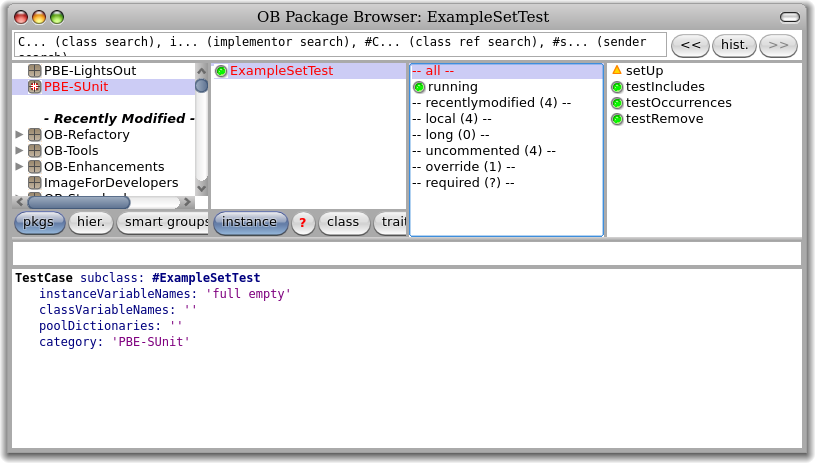
\includegraphics[width=\linewidth]{browser-tests}
	\caption{Запуск тестов \sunit из браузера}
	\figlabel{browser-tests}
  \end{center}
\end{figure}

%You can also select sets of test suites to run,
Также вы можете выбрать несколько наборов тестов для выполнения
%and obtain a more detailed log of the results using the \sunit \emphind{Test Runner},
и получить детальный лог, воспользовавшись \sunit \emphind{Test Runner},
%which you can open by selecting \menu{World \go Test Runner}.
который вы можете открыть выбрав \menu{World \go Test Runner}.
%The \emph{TestRunner}, shown in \figref{test-runner}, is designed 
\emph{TestRunner}, показанный на \figref{test-runner}, разработан для того,
%to make it easy to execute groups of tests.
чтобы сделать выполнение групп тестов легким и понятным.
%The left-most pane lists all of the categories that contain test classes
В списке на самой левой панели отображаются все категории, в которых присутствуют тестовые классы
%(\ie subclasses of \ct{TestCase});
(т.е. подклассы класса \ct{TestCase});
%when some of these categories are selected, the test classes that they contain appear in the pane to the right.
тестовые классы выбранных категорий отображаются в списке справа от списка категорий.
%Abstract classes are italicized, and the test class hierarchy is shown by indentation,
Абстрактные классы выделены курсивом, иерархия тестовых классов представлена с помощью отступов,
%so subclasses of \ct{ClassTestCase} are indented more than subclasses of \ct{TestCase}.
так что подклассы класса \ct{ClassTestCase} имеют больший отступ, чем подклассы класса \ct{TestCase}. 

\begin{figure}[tbh]
  \begin{center}
	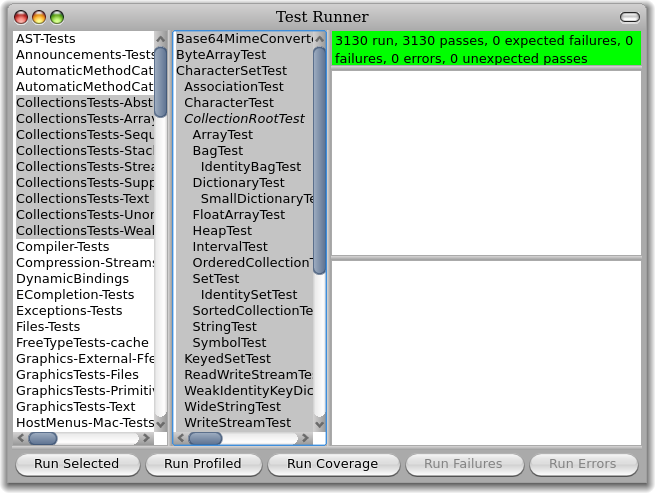
\includegraphics[width=\linewidth]{test-runner}
	\caption{The \pharo \sunit Test Runner}
	\figlabel{test-runner}
  \end{center}
\end{figure}

%\dothis{Open a Test Runner, select the category \menu{MyTest}, and click the \button{Run Selected} button.}
\dothis{Откройте Test Runner, выберите категорию \menu{MyTest}, и нажмите кнопку \button{Run Selected}.}

% ON: With OB, you don't need this.
%You can also run a single test by executing a \menu{print it} on the following code: \ct{ExampleSetTest run: #testRemove}.  
%We usually include an executable comment in our test methods that allows us to run them
%with a \menu{do it} from the browser, as shown in \mthref{ExampleSetTestTestRemoveii}.

%\needlines{6}
%\begin{method}[ExampleSetTestTestRemoveii]{Executable comments in test methods}
%ExampleSetTest>>>testRemove
%	"self run: #testRemove"
%	full remove: 5.
%	self assert: (full includes: 6).
%	self deny: (full includes: 5)
%\end{method}

%\dothis{Introduce a bug in \ct{ExampleSetTest>>>testRemove} and run the tests again.
%For example, change \ct{5} to \ct{4}.}
\dothis{Попробуйте специально допустить ошибку в \ct{ExampleSetTest>>>testRemove} и запустите тесты снова. 
Например, поменяйте \ct{5} на \ct{4}.}

%The tests that did not pass (if any) are listed in the right-hand panes of the \emph{Test Runner};
Несработавшие тесты (если таковые имеются) отображены на самых правых панелях;
%if you want to debug one, to see why it failed, just click on the name.
если вы хотите приступить к отладке или посмотреть в чем ошибка, просто нажмите на соответствующее имя теста.

%Alternatively, you can execute the following expressions:
%\begin{code}{}
%(ExampleSetTest selector: #testRemove) debug
%\end{code}
%or
%\begin{code}{}
%ExampleSetTest debug: #testRemove
%\end{code}

%---------------------------------------------------------
%\subsection{Step 5: interpret the results}
\subsection{Шаг 5: интерпретирование результатов}

%The method \mthind{TestCase}{assert:}\,, which is defined in the class \ct{TestCase},
Метод \mthind{TestCase}{assert:}\,, который определён в классе \ct{TestCase},
%expects a boolean argument, usually the value of a tested expression.
ожидает аргумент типа boolean, обычно это результат тестируемого выражения.
%When the argument is true, the test passes; when the argument is false, the test fails.
Если аргумент равен true, то тест сработал, если false, то не сработал.

%There are actually three possible outcomes of a test.
Фактически, есть три возможных результата выполнения теста.
%The outcome that we hope for is that all of the assertions in the test are true,
Первый состоит в том, что все утверждения в тесте сработали,
%in which case the test passes. In the test runner, when all of the tests pass,
таким образом, и сам тест сработал. В тестировщике (test runner), когда все тесты сработали,
%the bar at the top turns green. 
верхняя полоса окрашивается в зеленый цвет.
%However, there are also two kinds of thing that can go wrong when you run a test.
Однако есть ещё две неприятности, которые могут произойти при запуске теста.
%Most obviously, one of the assertions can be false, causing the test to \emph{fail}.
Чаще всего, одно из утверждений (assert) в тесте не срабатывает, а значит и тест не сработал.
%However, it is also possible that some kind of error occurs during the execution of the test,
Также возможна третья ситуация, когда возникает ошибка во время выполнения теста,
%such as a \emph{message not understood} error
например, \emph{message not understood} (неопознанное сообщение)
%or an \emph{index out of bounds} error.
или \emph{index out of bounds} (индекс за пределами массива).
%If an error occurs, the assertions in the test method may not have been executed at all,
В таком случае, утверждения в тесте могут вообще не выполниться (не запуститься),
%so we can't say that the test has failed; nevertheless, something is clearly wrong!
так что мы не можем сказать, что тест провален; тем не менее, такого точно не должно быть!
%In the {test runner}, failing tests cause the bar at the top to turn yellow, 
В тестировщике (test runner) такая ситуация обозначается желтой полосой сверху,
%and are listed in the middle pane on the right, whereas erroneous tests cause the bar to turn red, 
%and are listed in the bottom pane on the right.
такие тесты отображается на панели справа посередине, в то время, как несработавшие тесты отображаются в панели справа снизу и полоса сверху становится красной.

%\dothis{Modify your tests to provoke both errors and failures.}
\dothis{Измените свои тесты, чтобы спровоцировать обе ситуации.}

%=================================================================
%\section{The \SUnit cook book}
\section{Кулинарная книга \SUnit}

%This section will give you more details on how to use \SUnit.
Этот раздел более подробно рассказывает, как использовать \SUnit.
%If you have used another testing framework such as \JUnit\footnote{\url{http://junit.org}},
Если вы использовали другие инструменты тестирования, например \JUnit\footnote{\url{http://junit.org}},
%much of this will be familiar, since all these frameworks have their roots in \SUnit.
то многое покажется вам знакомым, поскольку они все берут свои корни из \SUnit.
%Normally you will use \SUnit's GUI to run tests,
Для запуска тестов чаще всего вы будете использовать \SUnit интерфейс (GUI),
%but there are situations where you may not want to use it.
но в некоторых ситуациях вам не захочется его использовать.

%---------------------------------------------------------
%\subsection{Other assertions}
\subsection{Другие утверждения}

%In addition to \ct{assert:} and \ct{deny:}, there are several other methods that can be used to make assertions.
В дополнение к \ct{assert:} и \ct{deny:}, вы можете использовать и другие методы утверждения в тесте.

%First, \mthind{TestCase}{assert:description:} and \mthind{TestCase}{deny:description:} 
Во-первых, \mthind{TestCase}{assert:description:} и \mthind{TestCase}{deny:description:},
%take a second argument which is a message string that can be used to describe the reason for the failure, 
которые имеют второй аргумент для описания причины ошибки,
%if it is not obvious from the test itself. These methods are described in~\secref{descriptionStrings}.
если таковая не очевидна из самого теста. Эти методы описаны в \secref{descriptionStrings}.

%Next, \sunit provides two additional methods, \mthind{TestCase}{should:raise:} and
Во-вторых, SUnit предоставляет два дополнительных метода: \mthind{TestCase}{should:raise:} и
%\mthind{TestCase}{shouldnt:raise:} for testing exception propagation.
\mthind{TestCase}{shouldnt:raise:} для тестирования исключений.
%For example, you would use \ct{(self should: aBlock raise: anException)} 
Например, вы можете использовать \ct{(self should: aBlock raise: anException)}
%to test that a particular exception is raised during the execution of \ct{aBlock}.  
для тестирования частного исключения при выполнении блока \ct{aBlock}.
%\Mthref{ESTtestIllegal} illustrates the use of \mbox{\ct{should:raise:}.}
\Mthref{ESTtestIllegal} показывает использование \mbox{\ct{should:raise:}.}

%\dothis{Try running this test.}
\dothis{Попробуйте запустить этот тест.}
%Note that the first argument of the \ct{should:} and \ct{shouldnt:} methods is a \emphind{block}
Кстати, первым аргументом метода \ct{should:} и \ct{shouldnt:} является \emphind{блок},
%that \emph{contains} the expression to be evaluated.   
который \emph{содержит} в себе выражение для выполнения. 

%\begin{method}[ESTtestIllegal]{Testing error raising}
\begin{method}[ESTtestIllegal]{Тестирование возникновения исключения}
ExampleSetTest>>>testIllegal
	self should: [empty at: 5] raise: Error.
	self should: [empty at: 5 put: #zork] raise: Error
\end{method}

%\sunit is portable: it can be used from all dialects of \st.
\sunit легко портируется, так что вы можете использовать его на всех диалектах \st.
%To make \sunit portable, its developers factored-out the dialect-dependent aspects.
Для этого разработчики продумали зависимые от диалекта аспекты.
%The class method \cmind{TestResult class}{error} 
Метод \cmind{TestResult class}{error}
%answers the system's error class in a dialect-independent fashion. 
возвращает ответ в виде системного класса error в независимом от диалекта представлении.
%You can take advantage of this: if you want to write tests that will work in any dialect of \st,
Если вы хотите воспользоваться этим преимуществом и писать независимые от диалекта Smalltalk тесты,
%instead of \mthref{ESTtestIllegal} you would write:
то вместо \mthref{ESTtestIllegal} напишите следующее:

\needlines{4}
%\begin{method}[portabletestillegal]{Portable error handling}
\begin{method}[portabletestillegal]{Портируемая обработка исключений}
ExampleSetTest>>>testIllegal
	self should: [empty at: 5] raise: TestResult error.
	self should: [empty at: 5 put: #zork] raise: TestResult error
\end{method}

%\dothis{Give it a try.}
\dothis{Попробуйте.}

%---------------------------------------------------------
%\subsection{Running a single test}
\subsection{Запуск отдельного теста}
%Normally, you will run your tests using the Test Runner.
Чаще всего, вы будете выполнять тесты, используя Test Runner.
%If you don't want to launch the Test Runner from the \menu{open\,\ldots} menu,
Если вы не хотите запускать Test Runner из меню \menu{open\,\ldots},
%you can execute \ct{TestRunner open} as a \menu{print it}.
то вы можете выполнить \ct{TestRunner open} в workspace из меню \menu{print it}.

%You can run a single test as follows.
Вы можете запустить отдельный тест следующим образом

\begin{code}{}
ExampleSetTest run: #testRemove --> 1 run, 1 passed, 0 failed, 0 errors
\end{code}

%---------------------------------------------------------
%\subsection{Running all the tests in a test class}
\subsection{Запуск всех тестов класса}

%Any subclass of \ct{TestCase} responds to the message \ct{suite},
Все подклассы класса \ct{TestCase} отвечают на сообщение \ct{suite},
%which will build a test suite that contains all the methods in the class
создающее набор тестов,
%whose names start with the string ``\ct{test}''.
который содержит все методы класса, начинающиеся со слова ``\ct{test}''.
%To run the tests in the suite, send it the message \ct{run}. For example:
Чтобы запустить этот набор тестов на выполнение отправьте ему сообщение \ct{run}. Например:

\begin{code}{}
ExampleSetTest suite run --> 5 run, 5 passed, 0 failed, 0 errors
\end{code}

%---------------------------------------------------------
%\subsection{Must I subclass TestCase?}
\subsection{Всегда ли делать подкласс от TestCase?}

%In \JUnit{} you can build a \clsind{TestSuite} from an arbitrary class 
В \JUnit{} вы можете создать \clsind{TestSuite} из любого класса,
%containing \ct{test*} methods.
содержащего методы, имя которых начинается с \ct{test*}.
%In \st you can do the same but you will then have to create a suite by hand 
Вы можете сделать то же самое и здесь, но вам придется создавать набор вручную,
%and your class will have to implement all the essential \ct{TestCase} methods like \ct{assert:}.
и ваш класс должен реализовывать методы класса \ct{TestCase}, например, \ct{assert:}.
%We recommend that you not try to do this. The framework is there: use it.
Мы рекомендуем вам работать с уже существующим \SUnit.

%=================================================================
%\section{The SUnit framework}
\section{SUnit фреймворк}

%\sunit consists of four main classes: \clsind{TestCase}, \clsind{TestSuite}, \clsind{TestResult},
Как показано на \figref{sunit-classes} \SUnit содержит четыре основных класса: \clsind{TestCase},
%and \clsind{TestResource}, as shown in \figref{sunit-classes}.
\clsind{TestSuite}, \clsind{TestResult}, и \clsind{TestResource}.
%The notion of a \emph{test resource} was introduced in \sunit 3.1 to represent a resource
Понятие ресурс теста (\emph{test resource}) было введено в \secref{introdution}, 
%that is expensive to set-up but which can be used by a whole series of tests.
описывающее ресурс, который можно использовать в каждом тесте.
%A \ct{TestResource} specifies a \ct{setUp} method that is executed just once before a suite of tests;
\ct{TestResource} имеет метод \ct{setUp}, который выполняется один раз перед запуском набора тестов,
%this is in distinction to the \ct{TestCase>>>setUp} method, which is executed before each test.
в этом состоит отличие от метода \ct{TestCase>>>setUp}, который выполняется перед каждым тестом.

\begin{figure}[htb]
  \begin{center}
		{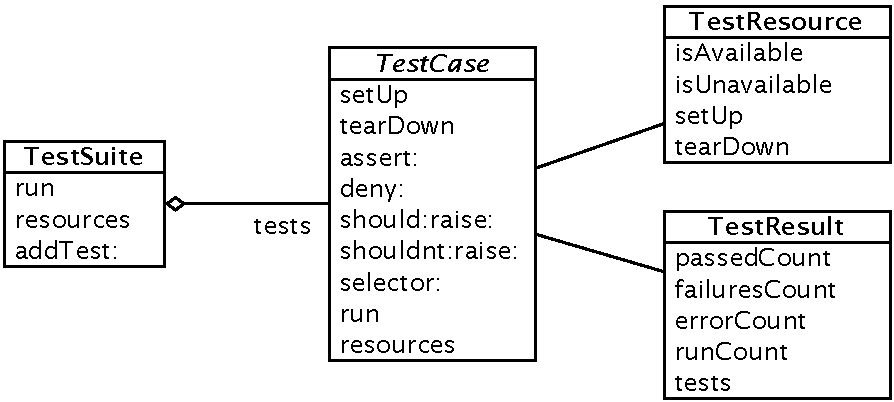
\includegraphics[width=0.8\textwidth]{sunit-classes}}
%	\caption{The four classes representing the core of \SUnit}
	\caption{Ядро \SUnit состоит из четырех классов}
	\figlabel{sunit-classes}
  \end{center}
\end{figure}


%---------------------------------------------------------
\subsection{TestCase}

%\clsindmain{TestCase} is an abstract class that is designed to be subclassed;
\clsindmain{TestCase} является абстрактным классом, и его назначение - быть предком;
%each of its subclasses represents a group of tests that share a common context (that is, a test suite).
каждый подкласс представляет собой группу тестов с одним контекстом (средой выполнения).
%Each test is run by creating a new instance of a subclass of \ct{TestCase},
При запуске теста создается экземпляр подкласса от \ct{TestCase},
%running \mthind{TestCase}{setUp}, running the test method itself, and then running \mthind{TestCase}{tearDown}.
выполняется \mthind{TestCase}{setUp}, выполняется тестовый метод, затем выполняется \mthind{TestCase}{tearDown}.

%The context is specified by instance variables of the subclass
Контекст определяется переменными экземпляра подкласса,
%and by the specialization of the method \ct{setUp}, which initializes those instance variables.
а также методом \ct{setUp}, который их инициализирует.
%Subclasses of \ct{TestCase} can also override method \ct{tearDown},
В подклассе класса \ct{TestCase} можно также переопределить метод \ct{tearDown},
%which is invoked after the execution of each test,
который выполняется после каждого теста,
%and can be used to release any objects allocated during \ct{setUp}.
и его можно использовать, чтобы освободить объекты, инициализированные в \ct{setUp}.

%---------------------------------------------------------
\subsection{TestSuite}

%Instances of the class \clsindmain{TestSuite} contain a collection of test cases.
Экземпляры класса \clsindmain{TestSuite} содержат коллекцию тестовых случаев.
%An instance of \ct{TestSuite} contains tests, and other test suites.
Экземпляр класса \ct{TestSuite} содержит сами тесты и наборы тестов.
%That is, a test suite contains sub-instances of \ct{TestCase} and \ct{TestSuite}.
То есть, набор тестов состоит из экземпляров класса \ct{TestCase} и класса \ct{TestSuite}.
%Both individual \lct{TestCase}s and \lct{TestSuite}s understand the same protocol,
Классы \lct{TestCase} и \lct{TestSuite} имеют один и тот же протокол (интерфейс),
%so they can be treated in the same way; for example, both can be \ct{run}.
так с ними можно работать одинаковым образом, например, и тот и другой имеют метод \ct{run}.
%This is in fact an application of the composite pattern in which \ct{TestSuite} is the composite
Фактически это реализация паттерна Composite, в котором \ct{TestSuite} – составной элемент,
%and the \ct{TestCase}s are the leaves\,---\,see \textit{Design Patterns}
а \ct{TestCase} – листья (смотрите «Паттерны проектирования» (\textit{Design Patterns}\cite{Gamm95a})
%for more information on this pattern\cite{Gamm95a}.
для более детальной информации).

%---------------------------------------------------------
\subsection{TestResult}

%The class \clsindmain{TestResult} represents the results of a \ct{TestSuite} execution.
Класс \clsindmain{TestResult} представляет собой результаты выполнения \ct{TestSuite} (набора тестов).
%It records the number of tests passed, the number of tests failed, and the number of errors signalled.
Он записывает количество сработавших и несработавших тестов, а также число ошибок выполнения.

%---------------------------------------------------------
\subsection{TestResource}
\seclabel{resource}

%One of the important  features of a suite of tests is that they should be independent of each other:
Одна из важных особенностей набора тестов в том, что они должны быть независимы друг от друга:
%the failure of one test should not cause an avalanche of failures of other tests that depend upon it,
провал одного теста не должен приводить к каскадному провалу всех зависящих от него тестов,
%nor should the order in which the tests are run matter.
а также последовательность запуска тестов не должна иметь значения.
%Performing \ct{setUp} before each test and \ct{tearDown} afterwards helps to reinforce this independence. 
Выполняющийся перед каждым тестом метод \ct{setUp} и после теста – \ct{tearDown} помогают убрать зависимости.

%However, there are occasions where setting up the necessary context is just too time-consuming
%for it to be practical to do once before the execution of each test.
Однако часто предустановка контекста перед каждым тестом расходует слишком много времени.
%Moreover, if it is known that the test cases do not disrupt the resources used by the tests,
Более того, если заранее известно, что тестовые случаи не изменяют используемые ресурсы,
%then it is wasteful to set them up afresh for each test;
то выставлять всё заново перед каждым тестом слишком расточительно;
%it is sufficient to set them up once for each suite of tests.
достаточно установить контекст один раз для одного набора тестов.
%Suppose, for example, that a suite of tests needs to query a database,
Предположим, что набору тестов требуется запрос к базе данных,
%or do some analysis on some compiled code.
или проанализировать скомпилированный код.
%In such cases, it may make sense to set up the database and open a connection to it,
В таких случаях перед запуском тестов имеет смысл установить соединение с базой данных,
%or to compile some source code, before any of the tests start to run.
или скомпилировать кусок исходного кода.

%Where should we cache these resources, so that they can be shared by a suite of tests?
Где же нам хранить эти ресурсы, чтобы набор тестов имел к ним доступ?
%The instance variables of a particular \ct{TestCase} sub-instance won't do,
Переменные экземпляра подкласса от \ct{TestCase} не подходит,
%because such an instance persists only for the duration of a single test.
потому что их область видимости ограничена отдельным тестом.
%A global variable would work, but using too many global variables pollutes the name space,
Глобальные переменные, конечно, будут работать, но они засоряют пространство имён,
%and the binding between the global and the tests that depend on it will not be explicit.
а также неочевидной будет связь между тестом и его глобальными переменными.
%A better solution is to put the necessary resources in a singleton object of some class.
Лучшее решение – это сложить все ресурсы в объект-одиночку (паттерн singleton) какого-либо класса.
%The class \clsindmain{TestResource} exists to be subclassed by such resource classes.
Класс \clsindmain{TestResource} существует для того, чтобы быть родителем таких классов.
%Each subclass of \lct{TestResource} understands the message  \ct{current},
Каждый потомок класса \lct{TestResource} понимает сообщение \ct{current},
%which will answer a singleton instance of that subclass.
которое возвращает экземпляр объекта-одиночки (singleton) для этого подкласса.
%Methods \ct{setUp} and \ct{tearDown} should be overridden in the subclass
Методы \ct{setUp} и \ct{tearDown} следует переопределить в подклассе,
%to ensure that the resource is initialized and finalized.
чтобы убедиться как в инициализации, так и в освобождении ресурса.

%One thing remains: somehow, \sunit has to be told which resources are associated with which test suite.
И последнее, \sunit должен знать какой ресурс относится к какому набору тестов.
%A resource is associated with a particular subclass of \ct{TestCase} 
%by overriding the \emph{class} method \ct{resources}.
Такая привязка осуществляется путем переопределения классового метода \ct{resources} в подклассе от \ct{TestCase}.
%By default, the resources of a \ct{TestSuite} are the union 
По умолчанию, ресурсы набора тестов \ct{TestSuite} – это объединение (union)
%of the resources of the \ct{TestCase}s that it contains.
ресурсов содержащихся в нем тестов \ct{TestCase}.

%Here is an example. We define a subclass of \ct{TestResource} called \ct{MyTestResource}
Приведем пример. Определим \ct{TestResource} – подкласс от \ct{MyTestResource} –
%and we associate it with \ct{MyTestCase} by specializing the class method \ct{resources}
и свяжем его с \ct{MyTestCase} путём определения метода resources на стороне класса,
%to return an array of the test classes that it will use.
чтобы он возвращал массив классов тестов, которые будут его использовать.

\needlines{8}
%\begin{classdef}[mytestresource]{An example of a TestResource subclass}
\begin{classdef}[mytestresource]{Пример подкласса от TestResource}
 TestResource subclass: #MyTestResource
	instanceVariableNames: ''

MyTestCase class>>>resources
	"associate the resource with this class of test cases"
	^{ MyTestResource }
\end{classdef}

%\needlines{10}
%\begin{classdef}[mytestresource]{An example of a TestResource subclass}
%TestResource subclass: #MyTestResource
%	instanceVariableNames: ''

%MyTestResource>>>setUp
%	"Set up resources here."

%MyTestResource>>>tearDown
%	"Tear down resources here."

%MyTestCase class>>>resources
%	"associate the resource with this class of test cases"
%	^{ MyTestResource }
%\end{classdef}

% \on{Do we really need the empty setUp and tearDown methods here?}

%=================================================================
%\section{Advanced features of SUnit}
\section{Продвинутые возможности SUnit}

%In addition to \ct{TestResource}, the current version of \sunit contains assertion description strings,
Кроме \ct{TestResource} текущая версия \sunit содержит описатели утверждений,
%logging support, and resumable test failures.
возможность ведения лога и возобновление выполнения теста после сбоя.

%---------------------------------------------------------
%\subsection{Assertion description strings}
\subsection{Описание утверждений}
\seclabel{descriptionStrings}

%The \ct{TestCase} assertion protocol includes a number of methods that allow the programmer
%to supply a description of the assertion.
Протокол утверждений в \ct{TestCase} позволяет программисту добавлять описания для утверждений.
%The description is a \ct{String}; if the test case fails, this string will be displayed by the test runner.
Описание – это строка (\ct{String}); если тест не сработает, то эта строка появится на экране.
%Of course, this string can be constructed dynamically.
Конечно, строку можно формировать динамически.

\begin{code}{}
| e |
e := 42.
self assert: e = 23
	description: 'expected 23, got ', e printString
\end{code}

%The relevant methods in \ct{TestCase} are:
Соответствующие методы в \ct{TestCase}:

\begin{code}{}
#assert:description:
#deny:description:
#should:description:
#shouldnt:description:
\end{code}
\cmindex{TestCase}{assert:description:}
\cmindex{TestCase}{deny:description:}
\cmindex{TestCase}{should:description:}
\cmindex{TestCase}{shouldnt:description:}

%---------------------------------------------------------
%\subsection{Logging support}
\subsection{Ведение лога}

%The description strings described above may also be logged to a \ct{Stream} such as the \ct{Transcript},
Строки описания, упомянутые выше, можно записать как лог в поток (\ct{Stream}), например, в \ct{Transcript}
%or a file stream. You can choose whether to log by overriding \cmind{TestCase}{isLogging} in your test class;
или в файл (файловый поток). Переопределите метод \cmind{TestCase}{isLogging} в классе,
%you must also choose where to log by overriding \cmind{TestCase}{failureLog} to answer an appropriate stream.
чтобы указать, когда вести лог, а \cmind{TestCase}{failureLog} возвращает поток для записи лога.

%---------------------------------------------------------
\subsection{Continuing after a failure}
\subsection{Продолжение после сбоя}

%\sunit also allows us to specify whether or not a test should continue after a failure.
В SUnit мы можем указать продолжить ли выполнение теста после сбоя или нет.
%This is a really powerful feature that uses the exception mechanisms offered by \st.
Это действительно полезная возможность, которая использует механизм исключений в \st.
%To see what this can be used for, let's look at an example.
Давайте рассмотрим пример, чтобы понять, как его использовать.
%Consider the following test expression:
Допустим, у нас есть следующее тестовое утверждение:

\begin{code}{}
aCollection do: [ :each | self assert: each even]
\end{code}

%In this case, as soon as the test finds the first element of the collection that isn't \ct{even}, the test stops.
В данном случае, как только будет достигнут первый нечетный элемент, тест прекратит цикл.
%However, we would usually like to continue, and see both how many elements, and which elements, 
Но, скорее всего, вам нужно найти все нечетные элементы, 
%aren't \ct{even}, and maybe also log this information. You can do this as follows:
а также записать эту информацию в лог. Можно поступить следующим образом:

\begin{code}{}
aCollection do:
	[:each |
	self
		assert: each even
		description: each printString , ' is not even'
		resumable: true]
\end{code}

%This will print out a message on your logging stream for each element that fails.
Этот код выводит сообщение в ваш лог для каждого несработавшего элемента.
%It doesn't accumulate failures, \ie if the assertion fails 10~times in your test method,
В то же время он не накапливает ошибки, т.е. если утверждение не сработает 10 раз,
%you'll still only see one failure. All the other assertion methods that we have seen are not resumable;
то вы увидите только одно сообщение. Остальные типы утверждений в тесте не восстанавливающиеся;
%\ct{assert: p description: s} is equivalent to \ct{assert: p description: s resumable: false}.
\ct{assert: p description: s} то же самое что и \ct{assert: p description: s resumable: false}.
\cmindex{Collection}{do:}
  
%=================================================================
%\section{The implementation of SUnit}
\section{Использование SUnit}

%The implementation of \sunit makes an interesting case study of a \st framework.
%Let's look at some key aspects of the implementation by following the execution of a test.
Давайте рассмотрим пример, чтобы получить представление о ключевых аспектах использования \sunit.

%---------------------------------------------------------
\subsection{Running one test}
\subsection{Запускаем отдельный тест}

%To execute one test, we evaluate the expression \ct{(aTestClass selector: aSymbol) run.}
Для этого выполните выражение \ct{(aTestClass selector: aSymbol) run.}

\begin{figure}[tbh]
  \begin{center}
		{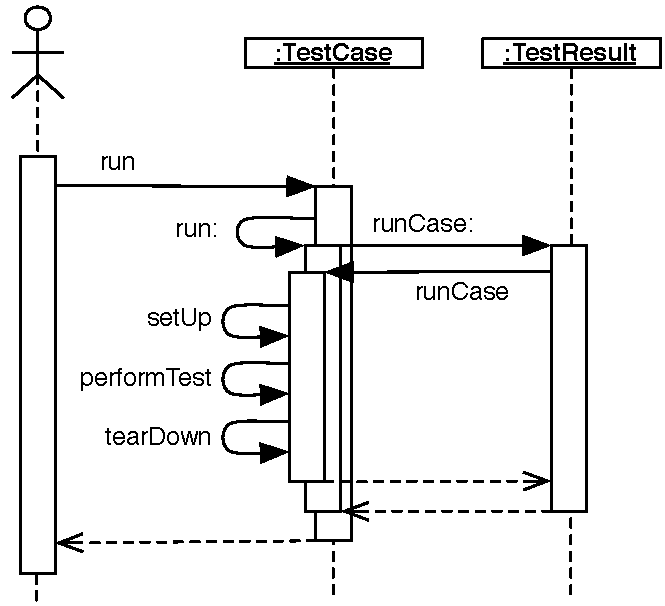
\includegraphics[width=0.7\textwidth]{sunit-scenario}}
%	\caption{Running one test}
	\caption{Запуск отдельного теста}	
	\figlabel{sunit-scenario}
  \end{center}
\end{figure}

%The method \cmind{TestCase}{run} creates an instance of \clsind{TestResult} 
Метод \cmind{TestCase}{run} создает экземпляр класса \clsind{TestResult},
%that will accumulate the results of the tests, then it sends itself the message \mthind{TestCase}{run:}.
который соберёт результаты тестов, а затем посылает себе сообщение \mthind{TestCase}{run:}.
%(See \figref{sunit-scenario}.)
(См. \figref{sunit-scenario}.)

\needlines{6}
%\begin{method}[tastecaserun]{Running a test case}
\begin{method}[tastecaserun]{Запуск теста}
TestCase>>>run
	| result |
	result := TestResult new.
	self run: result.
	^result
\end{method}

% Note that in a future release, the class of the \ct{TestResult} to
% be created will be returned by a method so that new
%\ct{TestResult} can be introduced. }

%The method \cmind{TestCase}{run:} sends the message \mthind{TestResult}{runCase:} to the test result:
Метод \cmind{TestCase}{run:} посылает сообщение \mthind{TestResult}{runCase:} результату теста:

%\begin{method}[testcaserun:]{Passing the test case to the test result}
\begin{method}[testcaserun:]{Передача теста в качестве параметра в тестовый результат}
TestCase>>>run: aResult
	aResult runCase: self
\end{method}

%The method \ct{TestResult>>>runCase:} sends the message \mthind{TestCase}{runCase} to an individual test, to 
%execute the test. \ct{TestResult>>>runCase} deals with any exceptions that may be raised during the execution of a 
%test, runs a \ct{TestCase} by sending it themessage \ct{runCase}, and counts the errors, failures and passes.
Метод \ct{TestResult>>>runCase:} запускает набор тестов, посылая ему сообщение \mthind{TestCase}{runCase}. 
\ct{TestResult>>>runCase} обрабатывает все исключения, которые могут возникнуть в процессе выполнения теста, а 
также ведет подсчет несработавших тестов, ошибок выполнения и успешных тестов.

%\begin{method}[testresultruncase]{Catching test case errors and failures}
\begin{method}[testresultruncase]{Обработка ошибок и сбоев в тесте}
TestResult>>>runCase: aTestCase
	| testCasePassed |
	testCasePassed := true.
	[[aTestCase runCase] 
			on: self class failure
			do: 
				[:signal | 
				failures add: aTestCase.
				testCasePassed := false.
				signal return: false]]
					on: self class error
					do:
						[:signal |
						errors add: aTestCase.
						testCasePassed := false.
						signal return: false].
	testCasePassed ifTrue: [passed add: aTestCase]
\end{method}

%The method \ct{TestCase>>>runCase} sends the messages \mthind{TestCase}{setUp}
%and \mthind{TestCase}{tearDown} as shown below.
Метод \ct{TestCase>>>runCase} посылает сообщения \mthind{TestCase}{setUp}
и \mthind{TestCase}{tearDown} следующим образом:

\needlines{3}
%\begin{method}[testcaseruncase]{Test case template method}
\begin{method}[testcaseruncase]{Шаблон метода в TestCase}
TestCase>>>runCase
	[self setUp.
	self performTest] ensure: [self tearDown]
\end{method}

%---------------------------------------------------------
%\subsection{Running a \lct{TestSuite}}
\subsection{Запуск набора тестов \lct{TestSuite}}

%To run more than one test, we send the message \ct{run} to a \ct{TestSuite} that contains the relevant tests. 
Чтобы запустить более одного теста, мы посылаем сообщение \ct{run} соответствующему набору тестов \ct{TestSuite}.
%\ct{TestCase class} provides some functionality to build a test suite from its methods.
В классе \ct{TestCase} присутствует некоторая функциональность для построения набора тестов.
%The expression \ct{MyTestCase buildSuiteFromSelectors} returns a suite containing all the tests
%defined in the {\ct{MyTestCase} class.
Выражение \ct{MyTestCase buildSuiteFromSelectors} возвратит набор тестов, определённых в классе \ct{MyTestCase}.
%The core of this process is   

%\begin{method}[testcasetestselectors]{Auto-building the test suite}
\begin{method}[testcasetestselectors]{Автоматическое построение набора тестов}
TestCase class>>>testSelectors 
	^self selectors asSortedCollection asOrderedCollection select: [:each | 
		('test*' match: each) and: [each numArgs isZero]]
\end{method}
\cmindex{MyTestCase class}{buildSuiteFromSelectors}

%The method \cmind{TestSuite}{run} creates an instance of \ct{TestResult}, verifies that all the resources are available, and then sends itself the message \mthind{TestSuite}{run:}, which runs all the tests in the suite.
Метод \cmind{TestSuite}{run} создает экземпляр класса \ct{TestResult}, проверяет доступность ресурсов, после чего посылает самому себе сообщение \mthind{TestSuite}{run:}, которое и запускает все тесты в наборе.
%All the resources are then released.
После этого все ресурсы освобождаются.

\begin{method}[testsuiterun]{Running a test suite}
\begin{method}[testsuiterun]{Выполнение набора тестов}
TestSuite>>>run
	| result |
 	result := TestResult new.
	self resources do: [ :res |
		res isAvailable ifFalse: [^res signalInitializationError]].
	[self run: result] ensure: [self resources do: [:each | each reset]].
	^result
\end{method}

%\begin{method}[testsuiterun:]{Passing the test result to the test suite}
\begin{method}[testsuiterun:]{Передача результата теста в набор тестов}
TestSuite>>>run: aResult
	self tests do: [:each | 
		self changed: each.
		each run: aResult].
\end{method}

%The class \clsind{TestResource} and its subclasses keep track of their currently created instances (one per class) that can be accessed and created using the class method \mthind{TestResource class}{current}.
Класс \clsind{TestResource} и его подклассы следят за своими экземплярами (один экземпляр на класс), чтобы классовый метод \mthind{TestResource class}{current} работал как для доступа к ресурсу, так и для создания нового экземпляра (если такового нет).
%This instance is cleared when the tests have finished running and the resources are reset.
Экземпляр удаляется после того, как все связанные с ним тесты закончили своё выполнение.

%The resource availability check makes it possible for the resource to be re-created if needed, as shown in the class method \cmind{TestResource class}{isAvailable}.
С помощью проверки доступности ресурса можно создать его заново, как показано в классовом методе \cmind{TestResource class}{isAvailable}.
%During the \ct{TestResource} instance creation, it is initialized and the method \mthind{TestResource}{setUp} is invoked.
Во время создания экземпляра класса \ct{TestResource} происходит инициализация, а также вызов метода \mthind{TestResource}{setUp}.

%(Note it may happen that your version of \sunit 3.0 does
%not correctly initialize the resource.  A version with this bug
%circulated a lot.  Verify that \ct{TestResource}
%\ct{class>>>new} calls the method \ct{initialize}).

\needlines{4}
%\begin{method}[testresourceisavailable]{Test resource availability}
\begin{method}[testresourceisavailable]{Доступность ресурса теста}
TestResource class>>>isAvailable
	^self current notNil and: [self current isAvailable]
\end{method}
%\begin{method}[testresourcecurrent]{Test resource creation}
\begin{method}[testresourcecurrent]{Создание ресурса теста}
TestResource class>>>current
	current isNil ifTrue: [current := self new].
	^current
\end{method}
%\begin{method}[restresourceinitialize]{Test resource initialization}
\begin{method}[restresourceinitialize]{Инициализация ресурса теста}
TestResource>>>initialize
	super initialize.
	self setUp
\end{method}
%=================================================================
%\section{Some advice on testing}
\section{Полезные советы}

%While the mechanics of testing are easy, writing good tests is not.
Механика тестирования довольно простая, чего не скажешь о навыке создания хороших тестов.
%Here is some advice on how to design tests.
Вот несколько советов.

\begin{description}
%\item[Self-contained tests.] You do not
%  want to have to change your tests  each time you change your code, so try to write the tests
%  so that they are self-contained.  This can be difficult, but pays off in the
%  long term.  Writing tests in terms of stable interfaces supports
%  self-contained tests.
%  \on{I have no idea what you are trying to tell me.
%  What specifically should I do or not do?
%  Give an example!}

%\item[Do not over-test.] Try to build your tests so that they do not
%  overlap.  It is annoying to have many tests covering the same
%  functionality, because one bug in the code will then break many tests at the same time.
%  This is covered by Black's rule, below.

\index{Feathers, Michael}
%\item[Feathers' Rules for Unit tests.]
\item[Правила Физера для модульного тестирования.]
%Michael Feathers, an  agile process consultant and author, writes:\footnote{See
Майкл Физер (Michael Feathers), автор книг и консультант по гибкому программированию, пишет:\footnote{См.    \url{http://www.artima.com/weblogs/viewpost.jsp?thread=126923}. 9 September 2005} 
  \begin{quotation}
  \noindent
  {\it
%  A test is not a unit test if:
Тест не является модульным, если:
  \begin{itemize}
%	\item it talks to the database,
	\item он обращается к базе данных,	
%	\item it communicates across the network,
	\item он передает данные по сети,	
%	\item it touches the file system,
	\item он взаимодействует с файловой системой,
%	\item it can't run at the same time as any of your other unit tests, or
	\item его нельзя запустить в то же время, что и другие модульные тесты	
%	\item you have to do special things to your environment (such as editing config files) to run it.
	\item вы должны изменить окружение (контекст) (например, конфигурационный файл), чтобы запустить его.	
 \end{itemize}
%Tests that do these things aren't bad.
Подобные тесты не являются плохими.
%Often they are worth writing, and they can be written in a unit test harness.
Даже если их тяжело писать, и они не укладываются в модульное тестирование.
%However, it is important to be able to separate them from true unit tests so that we can keep a set of tests that we can run fast whenever we make our changes.
Тем не менее, их необходимо отделять от настоящих модульных тестов для того, чтобы проверка набора модульных тестов была быстрой всякий раз, когда мы вносим изменения.
 }
  \end{quotation}
%Never get yourself into a situation where you don't want to run your unit test suite because it takes too long.   
Избегайте ситуации, когда вы не хотите запускать набор тестов, потому что он долго выполняется.

%\item[Unit Tests \textit{vs.}\ Acceptance Tests.]
\item[Модульные тесты \textit{против}\ приёмочных тестов.]
%Unit tests capture one piece of functionality, and as such make it easier to identify bugs in that functionality.
Модульные тесты покрывают небольшой кусок функциональности, поэтому там легко исправить ошибку.
%As far as possible try to have unit tests for each method that could possibly fail, and group them per class.
Старайтесь иметь тесты на каждый ненадёжный метод и группируйте их в классы.
%However, for certain deeply recursive or complex setup situations,
Однако для действительно сложных ситуаций проще писать тесты в виде сценария выполнения программы,
%it is easier to write tests that represent a scenario in the larger application; these are called acceptance 
такие тесты называются приемочными или функциональными.
%tests or functional tests. Tests that break Feathers' rules may make good acceptance tests.
Из тестов, нарушающих правила Физера, могут получиться хорошие приемочные тесты.
%Group acceptance tests according to the functionality that they test.
Группируйте приемочные тесты в соответствии с функциональностью, которую они покрывают.
%For example, if you are writing a compiler, you might write acceptance tests
Например, если вы пишете компилятор, то вы можете написать приемочные тесты,
%that make assertions about the code generated for each possible source language statement.
которые проверяют код, сгенерированный для каждого выражения исходного языка.
%Such tests might exercise many classes, and might take a long time to run because they touch the 
Подобные тесты задействуют множество классов и могут занимать продолжительное время
%file system. You can write them using \sunit, but you won't want to run them each time you make a small change,
из-за работы с файловой системой. Вы пожжете писать их с помощью \sunit, но вы не захотите их запускать каждый раз,
%so they should be separated from the true unit tests.
когда вы немного изменили код, поэтому их нужно хранить отдельно от настоящих модульных тестов. 
 
%\item[Black's Rule of Testing.]

%For every test in the system, you should be able to identify some property
%for which the test increases your confidence.
Для каждого теста в системе должна быть своя зона ответственности (кусок кода).
%It's obvious that there should be no important property that you are not testing.
Очевидно, что все важные участки кода должны быть протестированы.
%This rule states the less obvious fact that there should be no test that does not add value to the system
%by increasing your confidence that a useful property holds.
Данное правило отражает менее очевидный факт, что не должно быть тестов, которые тестируют одно и то же.
%For example, several tests of the same property do no good. In fact, they do harm in two ways.
Например, несколько тестов одного свойства это нехорошо. Такие тесты даже вредны:
%First, they make it harder to infer the behaviour of the class by reading the tests. 
становится труднее понять поведение класса по его тестам,
%Second, because one bug in the code might then break many tests,
%they make it harder to estimate how many bugs remain in the code.
а также одна ошибка может «завалить» множество тестов за раз.
%So, have a property in mind when you write a test.
Не упускайте общую картину, когда пишите тест.
\end{description}

%\section{Extending \SUnit}
%\seclabel{extending}

%In this section we will explain how to extend \sunit so that it uses
%a \ct{setUp} and \ct{tearDown} that are shared by all of the
%tests in a \ct{TestCase} subclass.  We will define a new sublass
%of \ct{TestCase} called \ct{SharingSetUpTestCase}, and a
%subclass of \ct{SharingSetUpTestCase} called \ct{SharedOne}.
%We will also need to define a new subclass of \ct{TestSuite}
%called \ct{SharedSetUpTestSuite}, and we will make some minor
%adjustments to \ct{TestCase}.

%Our tests will be in \ct{SharedOne}.  When we execute
%\begin{script}
%Transcript clear.
%SharedOne suite run
%\end{script}
%we will obtain the following trace.
%\begin{code}{}
%SharedOne>>>setUp
%SharedOne class>>>sharedSetUp
%SharedOne>>>testOne
%SharedOne>>>tearDown
%SharedOne>>>setUp
%SharedOne>>>testTwo
%SharedOne>>>tearDown
%SharedOne class>>>sharedTearDown
%2 run, 2 passed, 0 failed, 0 errors
%\end{code}
%You can see that the shared code is executed just once for both
%tests.

%\subsection{\ct{SharedSetUpTestCase}}

%The extension of the \sunit framework is based on the introduction
%of two classes: \ct{SharedSetUpTestCase} and
%\ct{SharedSetUpTestSuite}.  The basic idea is to use a flag that
%is flushed (cleared) after a certain number of tests have been run.
%The class \ct{SharedSetUpTestCase} defines one instance variable
%that indicates whether each test is run individually or in the context
%of a shared \ct{setUp} and \ct{tearDown}.  There are also two
%class instance variables.  One indicates the number of tests for which
%the shared \ct{setUp} should be in effect, and the other indicates
%whether the shared \ct{setUp} is in effect.
%\begin{method}[xxx]{xxx}
%SharedSetUpTestCase
%	superclass: TestCase
%	instanceVariableNames: 'runIndividually '
%	classInstanceVariableNames: 'numberOfTestsToTearDown
%								 sharedSetUp '
%\end{method}
%\ct{suiteClass} is used by \ct{TestCase} to determine the
%suite that is running.
%\begin{method}[xxx]{xxx}
%SharedSetUpTestCase class>>>suiteClass
%	^SharedSetUpTestSuite
%\end{method}
%\begin{method}[xxx]{xxx}
%SharedSetUpTestCase class>>>sharedSetUp
%	"A subclass should only override this hook to define
%	 a sharedSetUp"
%\end{method}
%\begin{method}[xxx]{xxx}
%SharedSetUpTestCase class>>>sharedTearDown
%	"Here we specify the teardown of the shared setup"
%\end{method}
%\begin{method}[xxx]{xxx}
%SharedSetUpTestCase class>>>flushSharedSetUp
%	sharedSetUp := nil
%\end{method}
%The \ct{SharedSetUpTestCase} class is initialized with the number
%of tests for which the shared \ct{setUp} should be in effect.
%\begin{method}[xxx]{xxx}
%SharedSetUpTestCase class>>>armTestsToTearDown: aNumber
%	self flushSharedSetUp.
%	numberOfTestsToTearDown := aNumber.
%\end{method}
%Every time a test is run, the method \ct{anothertestHasBeenRun} is
%invoked.  Once the specified number of tests is reached the
%\ct{sharedSetUp} is flushed and the \ct{sharedTearDown} is
%executed.
%\begin{method}[xxx]{xxx}
%SharedSetUpTestCase class>>>anotherTestHasBeenRun
%	"Everytimes a test is run this method is called,
%	 once all the tests of the suite
%	 are run the shared setup is reset"
%	numberOfTestsToTearDown := numberOfTestsToTearDown - 1.
%	numberOfTestsToTearDown isZero
%		ifTrue:
%			[self flushSharedSetUp.
%			self sharedTearDown]
%\end{method}
%When a test is run its \ct{setUp} is executed and it then it calls
%the class method \ct{privateSharedSetUp}.  This method will only
%invoke the \ct{sharedSetUp} if the \ct{sharedSetUp} test
%indicates that it hasn't been done yet.
%\begin{method}[xxx]{xxx}
%SharedSetUpTestCase class>>>privateSharedSetUp
%	sharedSetUp isNil
%		ifTrue:
%			[sharedSetUp := 1.
%			self sharedSetUp]
%\end{method}
%\begin{method}[xxx]{xxx}
%SharedSetUpTestCase>>>setUp
%	self class privateSharedSetUp
%\end{method}
%\begin{method}[xxx]{xxx}
%SharedSetUpTestCase>>>tearDown
%	self class anotherTestHasBeenRun
%\end{method}
%When a test case is created we assume that it will be run once.  We
%can change this later by invoking the method
%\ct{executedFromASuite}.
%\begin{method}[xxx]{xxx}
%SharedSetUpTestCase>>>setTestSelector: aSymbol
%	"Must do it this way because there is no initialize"

%	runIndividually := true.
%	super setTestSelector: aSymbol
%\end{method}
%\begin{method}[xxx]{xxx}
%SharedSetUpTestCase>>>executedFromASuite
%	runIndividually := false
%\end{method}
%The methods responsible for test execution are then specialized as
%follows.
%\begin{method}[xxx]{xxx}
%runIndividually
%	^runIndividually
%\end{method}
%\begin{method}[xxx]{xxx}
%SharedSetUpTestCase>>>armTearDownCounter
%	self runIndividually
%		ifTrue: [self class armTestsToTearDown: 1]
%\end{method}
%\begin{method}[xxx]{xxx}
%SharedSetUpTestCase>>>runCaseAsFailure
%	self armTearDownCounter.
%	super runCaseAsFailure
%\end{method}
%\begin{method}[xxx]{xxx}
%SharedSetUpTestCase>>>runCase
%	self armTearDownCounter.
%	super runCase
%\end{method}

%\subsection{\ct{SharedOne}}

%\ct{SharedOne} is a new class which inherits from
%\ct{SharingSetUpTestCase} as follows.  We define two simple tests
%\ct{testOne} and \ct{testTwo}.
%\begin{method}[xxx]{xxx}
%SharedOne
%	superclass: SharingSetUpTestCase
%\end{method}
%\begin{method}[xxx]{xxx}
%SharedOne>>>testOne
%	Transcript
%		show: 'SharedOne>>>testOne';
%		cr
%\end{method}
%\begin{method}[xxx]{xxx}
%SharedOne>>>testTwo
%	Transcript
%		show: 'SharedOne>>>testTwo';
%		cr
%\end{method}
%Then we define the methods \ct{setUp} and \ct{tearDown} that
%will be executed before and after the execution of the tests exactly
%in the same way as with non sharing tests.  Note however, the fact
%that with the solution we will present we have to explicitly invoke
%the \ct{setUp} method and \ct{tearDown} of the superclass.
%\begin{method}[xxx]{xxx}
%SharedOne>>>setUp
%	Transcript
%		show: 'SharedOne>>>setUp';
%		cr.
%	super setUp
%\end{method}
%\begin{method}[xxx]{xxx}
%SharedOne>>>tearDown
%	Transcript
%		show: 'SharedOne>>>tearDown';
%		cr.
%	super tearDown
%\end{method}
%Finally, we define the methods \ct{sharedSetUp} and
%\ct{sharedTearDown} that will be only executed once for the two
%tests.  Note that this solution assumes that the tests are not
%destructive to the shared fixture, but just query it.
%\begin{method}[xxx]{xxx}
%SharedOne class>>>sharedSetUp
%	Transcript
%		show: 'SharedOne class>>>sharedSetUp';
%		cr
%	"My set up here."
%\end{method}
%\begin{method}[xxx]{xxx}
%SharedOne class>>>sharedTearDown
%	Transcript
%		show: 'SharedOne class>>>sharedTearDown';
%		cr
%	"My tear down here."
%\end{method}

%\subsection{\ct{SharedSetUpTestSuite}}

%The \ct{SharedSetUpTestSuite} defines just one instance variable
%\ct{testCaseClass} and redefines the two methods necessary to run
%the test suite \ct{run:} and \ct{run}.
%\ct{checkAndArmSharedSetUp} initializes the number of tests to run
%before the shared \ct{tearDown} is executed.
%\begin{method}[xxx]{xxx}
%SharedSetUpTestSuite
%	superclass: TestSuite
%	instanceVariableNames: 'testCaseClass'
%\end{method}
%\begin{method}[xxx]{xxx}
%SharedSetUpTestSuite>>>checkAndArmSharedSetUp
%	self tests isEmpty
%		ifFalse: [self tests first class
%				 armTestsToTearDown: self tests size]
%\end{method}
%\begin{method}[xxx]{xxx}
%SharedSetUpTestSuite>>>run: aResult
%	self checkAndArmSharedSetUp.
%	^super run: aResult
%\end{method}
%\begin{method}[xxx]{xxx}
%SharedSetUpTestSuite>>>run
%	self checkAndArmSharedSetUp.
%	^super run
%\end{method}
%Finally the method \ct{addTest:} is specialized so that it marks
%all its tests with the fact that they are executed in a
%\ct{TestSuite} and checks whether all its tests are from the same
%class to avoid inconsistency.
%\begin{method}[xxx]{xxx}
%SharedSetUpTestSuite>>>addTest: aTest
%	"Sharing a setup only works if the test case
%	composing the test suite are from
%	the same class so we test it"

%	aTest executedFromASuite.
%	testCaseClass isNil
%		ifTrue: [testCaseClass := aTest class.
%				super addTest: aTest ]
%		ifFalse: [aTest class == testCaseClass
%				  ifFalse: [self error:
%						   'you cannot have test case of
%							different classes in
%							a SharingSetUpTestSuite'.]
%				  ifTrue: [super addTest: aTest]]
%\end{method}

%\subsection{Changes to \ct{TestCase}}

%In order for the above changes to work, you must make
%\ct{TestCase} aware of your new test suite.
%\begin{method}[xxx]{xxx}
%TestCase class>>>buildSuite
%	| suite |
%	^self isAbstract
%		ifTrue:
%			[suite := self suiteClass new.
%			suite name: self name asString.
%			self allSubclasses
%				do: [:each |
%					each isAbstract
%						ifFalse: [suite addTest:
%						  each buildSuiteFromSelectors]].
%			suite]
%		ifFalse: [self buildSuiteFromSelectors]
%\end{method}
%\begin{method}[xxx]{xxx}
%TestCase class>>>buildSuiteFromMethods: testMethods
%	^testMethods
%		inject: ((self suiteClass new)
%				name: self name asString;
%				yourself)
%		into:
%			[:suite :selector |
%			suite
%				addTest: (self selector: selector);
%				yourself]
%\end{method}
%If you have made all the changes correctly, you should be able to run
%your tests and see the results shown in section~\ref{sec:extending}.
%
%\section{Exercise}

%The previous section was designed to give you some insight into the
%workings of \SUnit.  You can obtain the same effect by using \SUnit's
%resources.

%Create new classes \ct{MyTestResource} and \ct{MyTestCase}
%which are subclasses of \ct{TestResource} and \ct{TestCase}
%respectively.  Add the appropriate methods so that the following
%messages are written to the \ct{Transcript} when you run your
%tests.

%\begin{method}[xxx]{xxx}
%MyTestResource>>>setUp has run.
%MyTestCase>>>setUp has run.
%MyTestCase>>>testOne has run.
%MyTestCase>>>tearDown has run.
%MyTestCase>>>setUp has run.
%MyTestCase>>>testTwo has run.
%MyTestCase>>>tearDown has run.
%MyTestResource>>>tearDown has run.
%\end{method}

%% You need to write the following six methods.

%% MyTestCase>>>setUp
%%	 Transcript
%%		 show: 'MyTestCase>>>setUp has run.';
%%		 cr

%% MyTestCase>>>tearDown
%%	 Transcript
%%		 show: 'MyTestCase>>>tearDown has run.';
%%		 cr

%% MyTestCase>>>testOne
%%	 Transcript
%%		 show: 'MyTestCase>>>testOne has run.';
%%		 cr

%% MyTestCase>>>testTwo
%%	 Transcript
%%		 show: 'MyTestCase>>>testTwo has run.';
%%		 cr

%% MyTestCase class>>>resources
%%	 ^Array with: MyTestResource

%% MyTestResource>>>setUp
%%	 Transcript
%%		 show: 'MyTestResource>>>setUp has run';
%%		 cr

%% MyTestResource>>>tearDown
%%	 Transcript
%%		 show: 'MyTestResource>>>tearDown has run.';
%%		 cr
%=================================================================
%\section{Chapter summary}
\section{Краткое содержание главы}

%This chapter explained why tests are an important investment in the future of your code.  
Эта глава объясняет, почему тесты являются важными инвестициями в ваш код.
%We explained in a step-by-step fashion how to define a few tests for the class \ct{Set}.
Мы пошагово объяснили создание нескольких тестов для класса \ct{Set}.
%Then we gave an overview of the core of the \sunit framework by presenting the classes \ct{TestCase}, 
Затем мы рассмотрели ядро Фреймворка \sunit классы \ct{TestCase},
%\ct{TestResult}, \ct{TestSuite} and \lct{TestResources}.
\ct{TestResult}, \ct{TestSuite} и \lct{TestResources}.
%Finally we looked deep inside \sunit by following the execution of a test and a test suite.
И в конце мы заглянули внутрь \sunit при выполнении теста и набора тестов.

\begin{itemize}
%  \item To maximize their potential, unit tests should be fast, repeatable, independent of any direct human interaction and cover a single unit of functionality.
\item Чтобы использовать весь потенциал модульных тестов, они должны быть быстрыми, повторяемыми, независимыми от прямого воздействия человека и покрывать отдельный кусочек функциональности.
%  \item Tests for a class called \ct{MyClass} belong in a class classed \ct{MyClassTest}, which should be introduced as a subclass of \lct{TestCase}.
\item Тесты для класса \ct{MyClass} записываются в класс \ct{MyClassTest}, который должен быть унаследован от класса \lct{TestCase}.
%  \item Initialize your test data in a \ct{setUp} method.
\item Инициализируйте тест в методе \ct{setUp}
%  \item Each test method should start with the word ``test''.
\item Имя метода каждого теста должно начинаться со слова ``test''
%  \item Use the \ct{TestCase} methods \ct{assert:}, \ct{deny:} and others to make assertions.
\item Создавая утверждения, используйте методы \ct{assert:}, \ct{deny:} и другие методы класса \ct{TestCase}
%  \item Run tests using the SUnit test runner tool (in the tool bar).
\item Запускайте тесты используя Test Runner в \sunit
\end{itemize}   

%=============================================================
\ifx\wholebook\relax\else
   \bibliographystyle{jurabib}
   \nobibliography{scg}
   \end{document}
\fi
%=============================================================
%%% Local Variables:
%%% coding: utf-8
%%% mode: latex
%%% TeX-master: t
%%% TeX-PDF-mode: t
%%% ispell-local-dictionary: "english"
%%% End:
